\documentclass[openany]{fast-nuces-bs}

% -- Core packages ------------------------------------------------------------
\usepackage{mathptmx}                  % Times Roman font
\usepackage[T1]{fontenc}
\usepackage{lipsum}
\usepackage{sectsty}
\usepackage{titlesec}
\usepackage{booktabs}
\usepackage{array}
\usepackage{algorithm2e}[ruled]
\usepackage{longtable}
\usepackage{pdflscape}
\usepackage{tabularx}
\usepackage{multirow}
\usepackage{xcolor}
\usepackage{listings}
\usepackage{caption}
\usepackage{enumitem}
\usepackage[expansion=false]{microtype}
\usepackage{float}
\usepackage{placeins}

% --- TikZ for system / architecture / flow diagrams -------------------------
\usepackage{tikz}
\usetikzlibrary{shapes.geometric, shapes.symbols, arrows.meta, positioning,
                fit, backgrounds, calc, decorations.pathreplacing,
                decorations.pathmorphing, shadows, patterns, chains, scopes}

% Common colour palette (consistent with the matplotlib evaluation figures).
\definecolor{coralGreen}{HTML}{0F9D58}
\definecolor{coralBlue}{HTML}{1976D2}
\definecolor{coralOrange}{HTML}{E67E22}
\definecolor{coralRed}{HTML}{C0392B}
\definecolor{coralGrey}{HTML}{9AA0A6}
\definecolor{coralTeal}{HTML}{14B8A6}
\definecolor{coralViolet}{HTML}{6D28D9}
\definecolor{coralYellow}{HTML}{F4B400}
\definecolor{coralLightGrey}{HTML}{F1F3F4}
\definecolor{coralBoxBlue}{HTML}{E3F2FD}
\definecolor{coralBoxGreen}{HTML}{E8F5E9}
\definecolor{coralBoxOrange}{HTML}{FFF3E0}
\definecolor{coralBoxRed}{HTML}{FFEBEE}
\definecolor{coralBoxViolet}{HTML}{EDE7F6}
\definecolor{coralBoxYellow}{HTML}{FFF8E1}

% Reusable styles for the diagrams.
\tikzset{
  coral/box/.style       = {rounded corners=2pt, draw=coralGrey!70, fill=coralLightGrey,
                             very thick, align=center, minimum height=8mm,
                             font=\small\sffamily, inner sep=4pt, drop shadow={opacity=0.10}},
  coral/stage/.style     = {coral/box, fill=coralBoxBlue,   draw=coralBlue!70,   text=black},
  coral/data/.style      = {coral/box, fill=coralBoxGreen,  draw=coralGreen!70,  text=black},
  coral/llm/.style       = {coral/box, fill=coralBoxViolet, draw=coralViolet!70, text=black},
  coral/api/.style       = {coral/box, fill=coralBoxOrange, draw=coralOrange!80, text=black},
  coral/ext/.style       = {coral/box, fill=coralBoxYellow, draw=coralYellow!90, text=black},
  coral/error/.style     = {coral/box, fill=coralBoxRed,    draw=coralRed!70,    text=black},
  coral/decision/.style  = {diamond, aspect=2, draw=coralOrange!80, fill=coralBoxOrange,
                             align=center, font=\small\sffamily, very thick, inner sep=2pt},
  coral/proc/.style      = {ellipse, draw=coralBlue!80, fill=coralBoxBlue, very thick,
                             align=center, font=\small\sffamily, minimum height=8mm, inner sep=3pt},
  coral/store/.style     = {draw=coralGreen!80, fill=coralBoxGreen, very thick,
                             align=center, font=\small\sffamily, minimum height=7mm, inner sep=3pt},
  coral/entity/.style    = {rectangle, draw=coralYellow!90, fill=coralBoxYellow, very thick,
                             align=center, font=\small\sffamily, minimum height=8mm, inner sep=4pt},
  coral/note/.style      = {draw=coralGrey!60, fill=white, align=left, font=\footnotesize\sffamily,
                             rounded corners=1pt, inner sep=3pt},
  coral/arrow/.style     = {-{Stealth[length=2.2mm]}, thick, draw=coralGrey!85},
  coral/arrowg/.style    = {-{Stealth[length=2.2mm]}, thick, draw=coralGreen!75},
  coral/arrowo/.style    = {-{Stealth[length=2.2mm]}, thick, draw=coralOrange!80},
  coral/arrowr/.style    = {-{Stealth[length=2.2mm]}, thick, draw=coralRed!80},
  coral/biarrow/.style   = {{Stealth[length=2.2mm]}-{Stealth[length=2.2mm]}, thick, draw=coralGrey!85},
  coral/dashed/.style    = {-{Stealth[length=2.2mm]}, thick, draw=coralGrey!85, dashed},
  coral/title/.style     = {font=\sffamily\bfseries, text=coralBlue!80!black},
  coral/sublabel/.style  = {font=\footnotesize\sffamily\itshape, text=coralGrey!50!black},
}

\RestyleAlgo{ruled}

% Loosen line-breaking so long technical strings (e.g. file paths,
% \texttt{...}) do not produce overfull hboxes.
\sloppy
\raggedbottom
\setlength{\emergencystretch}{6em}
\tolerance=9999
\hbadness=10000
\hfuzz=20pt

% -- Code listing styles -----------------------------------------------------
\definecolor{codebg}{RGB}{248,248,242}
\definecolor{codecomment}{RGB}{106,153,85}
\definecolor{codekeyword}{RGB}{0,0,180}
\definecolor{codestring}{RGB}{163,21,21}
\definecolor{codenumber}{RGB}{120,120,120}
\definecolor{coderule}{RGB}{200,200,210}

\lstdefinestyle{coral}{
  backgroundcolor=\color{codebg},
  basicstyle=\footnotesize\ttfamily,
  breakatwhitespace=false,
  breaklines=true,
  captionpos=b,
  commentstyle=\itshape\color{codecomment},
  keywordstyle=\bfseries\color{codekeyword},
  stringstyle=\color{codestring},
  numberstyle=\tiny\color{codenumber},
  numbers=left,
  numbersep=8pt,
  showspaces=false,
  showstringspaces=false,
  showtabs=false,
  tabsize=2,
  frame=single,
  rulecolor=\color{coderule},
  xleftmargin=12pt,
  framexleftmargin=10pt,
  aboveskip=8pt,
  belowskip=8pt,
}
\lstset{style=coral}

% -- Project metadata ---------------------------------------------------------
\department{Department of Computer Science}
\faculty{Computer Science}
\degreeyear{2026}
\degreemonth{May}
\degreename{Computer Science}
\campuscity{Islamabad}
\authorone{Ali Irfan}{21I-2572}
\authortwo{Nouman Hafeez}{21I-0416}
\authorthree{Rafay Khattak}{21I-0423}
\supervisor{Ms.\ Kainat Iqbal}
\sessionduration{2021--2026}
\cosupervisor{Ms.\ Saira Qamar}
\deanname{Dr.\ Dean Computing}
\directorname{Dr.\ Director of the Campus}
\hodname{Dr.\ Head of Computer Science Department}
\fypcoordinatorname{FYP Coordinator}
\title{CORAL: Consensus-Based Refinement and Output Realignment for Low-Resource Urdu ASR Post-Processing}

% Define abstract / acknowledgements as chapter*-style front matter
\newenvironment{abstract}
  {\chapter*{Abstract}\addcontentsline{toc}{chapter}{Abstract}\thispagestyle{plain}}
  {\par}
\newenvironment{acknowledgements}
  {\chapter*{Acknowledgements}\addcontentsline{toc}{chapter}{Acknowledgements}\thispagestyle{plain}}
  {\par}

\begin{document}

\begin{abstract}
Urdu, spoken by over 230 million people worldwide and the national language of Pakistan, remains a severely under-resourced language for Automatic Speech Recognition (ASR). Even the strongest publicly available multilingual models exhibit Word Error Rates (WER) above 13\% on read speech and approaching 20\% on conversational audio, limiting deployment in critical domains such as healthcare, education, accessibility, and legal documentation. We present \textbf{CORAL} (\emph{Consensus-Based Refinement / Cross-Model Output Realignment for Low-Resource Urdu ASR Post-Processing}), an inference-time post-processing pipeline that improves Urdu ASR accuracy without retraining any underlying acoustic model. CORAL consists of five stages: (i) Urdu-specific text normalisation that strips diacritics, resolves Arabic--Urdu Unicode conflation, and removes non-Urdu artefacts; (ii) a novel split-merge-aware alignment algorithm that uses weighted word-level Levenshtein distance to align companion-model hypotheses to a designated source transcript while classifying each chunk as SAME, SPLIT, MERGE, or NOISE; (iii) out-of-vocabulary (OOV) detection and correction using BK-tree fuzzy lookup combined with bi/tri-gram language-model candidate ranking over a half-million-word DuckDB corpus; (iv) position-wise majority voting with conservative tie-breaking and OOV substitution; and (v) an LLM-assisted refinement layer for fluency restoration, code-switching recovery, and named-entity handling. We evaluate CORAL on 2{,}995 Mozilla Common Voice Urdu utterances and 500 conversational Urdu clips. Starting from a 19.8\% Whisper-Large-v3 baseline on conversational speech, the full CORAL pipeline reaches 10.6\% WER --- a 46.5\% relative improvement --- and on the read-speech benchmark the robust pipeline reduces WER from 18.4\% to 14.3\% (Seamless-Large source). Our ablation study shows that every component contributes a measurable, additive gain. CORAL is delivered as a deployed FastAPI backend, a Next.js front-end with a four-pass user workflow, Kaggle-GPU notebooks self-registered through an ngrok-tunnelled registry, and an open evaluation framework.

\textbf{Keywords:} Urdu ASR, ensemble post-processing, split-merge alignment, weighted Levenshtein, BK-tree, out-of-vocabulary correction, majority voting, LLM post-processing, low-resource speech recognition.
\end{abstract}

\begin{acknowledgements}
We wish to express our deepest gratitude to our project supervisor \textbf{Ms.\ Kainat Iqbal} and co-supervisor \textbf{Ms.\ Saira Qamar} for their continuous guidance, technical insight, and generosity with their time throughout both iterations of this Final Year Project. We are grateful to the Department of Computer Science at FAST-NUCES Islamabad for the computational resources and academic environment that made this work possible. We acknowledge the open-source communities behind \textsc{HuggingFace Transformers}, \textsc{Whisper}, \textsc{SeamlessM4T}, \textsc{Wav2Vec2}, the Mozilla Common Voice corpus, and the Conversational Urdu benchmark, whose publicly available resources formed the foundation of our evaluation infrastructure. Finally, we thank the native Urdu-speaking annotators who produced and verified the ground-truth transcriptions used in the ablation study.
\end{acknowledgements}

\chapter{Introduction}
\label{chap:introduction}

This chapter establishes the scope of the CORAL project. We motivate the work by characterising the state of Urdu Automatic Speech Recognition (ASR), articulate the research problem and hypothesis, present the final framing of the proposed solution as it emerged across two iterations, set the project objectives and deliverables, and document software requirements. The chapter closes with a description of how the workload was distributed across the team. The detailed methodology, implementation, and empirical evaluation are deferred to Chapters~\ref{chap:approach} and~\ref{chap:implementation}.

\section{Background}
\label{sec:background}

Automatic Speech Recognition has experienced extraordinary progress over the past decade. Foundation models such as OpenAI's Whisper~\cite{radford2022whisper}, Meta's MMS~\cite{pratap2023mms}, and Meta's SeamlessM4T~\cite{seamlessm4t2023} now achieve sub-5\% Word Error Rate (WER) on widely-spoken languages such as English and Mandarin. This performance has unlocked production deployments in voice assistants, real-time captioning, healthcare dictation, and dictation-based accessibility tools.

Urdu is the national language of Pakistan, an official language of several Indian states, and the lingua franca of the South Asian subcontinent. It is spoken by more than 230~million people worldwide and is written in the Nastaliq variant of the Perso-Arabic script. Despite its demographic significance, Urdu remains severely under-represented in modern ASR research. The most comprehensive recent benchmark of multilingual ASR systems on Urdu, conducted by Arif et al.~\cite{arif2024wer}, reports that even the strongest models achieve WER above 13\% on read speech and approaching 20\% on conversational audio. This performance ceiling places critical Urdu ASR applications in healthcare, legal documentation, education, and assistive technology effectively out of reach.

Urdu poses several genuine difficulties to ASR systems that are absent from high-resource languages:

\begin{itemize}
  \item \textbf{Limited training data.} High-quality, large-scale, time-aligned Urdu speech corpora are scarce compared with English or Mandarin. Most multilingual models see Urdu only as a small minority of their training mixture.
  \item \textbf{Linguistic complexity.} Urdu has rich morphology, extensive use of loanwords from Arabic, Persian, and English, an elaborate verbal agreement system covering gender, number and case, and pervasive optional diacritics that are produced inconsistently by different ASR back-ends.
  \item \textbf{Code-switching.} Conversational Pakistani speech routinely alternates between Urdu and English at the word and phrase level, a distribution that monolingual ASR systems are not trained to handle.
  \item \textbf{Dialectal variation.} Multiple regional dialects with distinct acoustic and lexical properties coexist within both Pakistan and India.
  \item \textbf{Script heterogeneity.} The same phoneme can be represented by multiple Unicode code points drawn from both the Arabic and Urdu sub-blocks (e.g.\ Arabic KAF \texttt{U+0643} vs.\ Urdu KEHEH \texttt{U+06A9}). This causes word-level mismatches during alignment and WER computation even when the word is phonetically and semantically correct.
  \item \textbf{Word-boundary inconsistency.} Urdu ASR back-ends disagree systematically on word boundaries: a phrase that one model transcribes as a single token is often split into two or three tokens by another, or merged from multiple tokens into one. Naive word-level alignment misinterprets these segmentation events as substitutions or deletions, corrupting any downstream voting or fusion signal.
\end{itemize}

\subsection{Limitations of Single-Model and Naive-Ensemble ASR}
\label{ssec:single-model-limits}

Single-model ASR architectures, even when fine-tuned on Urdu, suffer from three well-documented limitations: (i)~\emph{deterministic predictions} -- they emit a single best hypothesis without considering plausible alternatives; (ii)~\emph{absent uncertainty signal} -- they provide no easily actionable mechanism to indicate confidence in their output; and (iii)~\emph{domain brittleness} -- models fine-tuned on read speech generalise poorly to conversational audio, code-switched speech, or dialectal variation. The natural response is to combine the outputs of several independently trained ASR systems, expecting that the errors of one model will be corrected by the consensus of others. This is appealing because it requires no retraining, can be deployed at inference time, and can leverage architecturally diverse models that make systematically different error types.

However, ensemble combination methods such as ROVER~\cite{fiscus1997rover} were designed for phonetically regular, space-delimited scripts such as English. Applied naively to Urdu, they fail in three concrete ways: they are confounded by Arabic--Urdu Unicode variants; they misinterpret word-boundary disagreements as deletions or insertions; and they degrade quality when the ensemble contains models of widely heterogeneous quality (the canonical ROVER failure mode). The CORAL project was motivated by the observation that solving these three Urdu-specific complications requires a purpose-built post-processing pipeline rather than a direct application of off-the-shelf ensemble methods.

\section{Problem Statement}
\label{sec:problem}

CORAL addresses the following research problem:

\begin{quote}
\itshape
Current state-of-the-art pre-trained ASR models for Urdu exhibit Word Error Rates between 13\% and 20\% on read and conversational benchmarks respectively, and degrade further on out-of-domain and code-switched speech. No widely available ASR back-end provides robust handling of Arabic--Urdu Unicode variation, word-boundary disagreement across architectures, or out-of-vocabulary proper nouns. Existing ensemble fusion techniques developed for English are not directly transferable, because they confound Unicode variants, segmentation disagreement, and quality heterogeneity. The community needs a post-processing pipeline that recovers from these failures at inference time, without requiring fine-tuning or any change to the underlying acoustic models.
\end{quote}

This research problem decomposes into three concrete challenges:

\begin{enumerate}
  \item \textbf{Script heterogeneity and segmentation disagreement.} Word-boundary inconsistency is not captured by word-level alignment alone, and Arabic--Urdu Unicode variation causes phonetically identical tokens to register as distinct words during voting and WER computation.
  \item \textbf{Out-of-vocabulary handling.} Proper nouns, named entities, and rare technical terms are systematically misrecognised by all available ASR back-ends but are precisely the tokens whose correct transcription matters most in downstream applications.
  \item \textbf{Linguistic coherence and code-switching.} Word-level voting, even when correctly aligned, cannot recover sentence-level fluency, restore code-switched English tokens, or resolve grammatical agreement errors that span longer than a few words.
\end{enumerate}

\subsection{Research Hypothesis}
\label{ssec:hypothesis}

\textit{The CORAL hypothesis}: Combining (i)~Urdu-specific Unicode normalisation, (ii)~weighted split-merge-aware alignment of multiple ASR hypotheses, (iii)~hybrid OOV detection and correction with BK-tree fuzzy lookup ranked by an n-gram language model, (iv)~conservative position-wise voting, and (v)~targeted LLM refinement of the voted output, is sufficient to substantially reduce WER over the strongest single-model baseline on both read-speech and conversational Urdu, without requiring any fine-tuning of the underlying acoustic models.

\section{Proposed Solution: Evolution of the CORAL Framework}
\label{sec:proposed-solution-overview}

The CORAL system was developed across two distinct iterations of the Final Year Project, and the framework's framing evolved meaningfully between them. We document this evolution explicitly so that the relationship between the FYP-1 design and the deployed FYP-2 system is unambiguous; the technical detail behind the final pipeline is presented in Chapter~\ref{chap:approach}.

\subsection{Iteration~1 Framing (FYP-1): ``Generate-and-Refine''}
\label{ssec:iter1-framing}

The original CORAL framing, presented in the FYP-1 final report, was a two-stage \emph{Generate-and-Refine} architecture. \textbf{Stage~1} deployed an ensemble of pre-trained ASR models (Whisper Large/Medium/Small and Wav2Vec2-XLSR Urdu), extracted architecture-specific word-level confidence scores from each, and produced four to five confidence-annotated hypotheses for each audio input. \textbf{Stage~2} fed these confidence-annotated hypotheses into a black-box instruction-tuned LLM (Alif-1.0-8B-Instruct, an Urdu-focused 8B-parameter model) using a structured prompt that asked the LLM to weight competing tokens by their reported confidences and emit a single corrected sentence. Iteration~1 established a strong baseline (Whisper-Large at 17.76\% WER on a 10-clip read-speech test set) and validated that the architecture-specific confidence-extraction methodology produced usable signals; Iteration~2 then implemented the LLM-correction stage and reported a 18.15\% WER on a controlled 20-sample synthetic dataset that probed three calibration regimes (well-calibrated, overconfident, underconfident) and three error types (substitution, insertion, deletion).

\subsection{Iteration~2 Reframing (FYP-2): A Five-Stage Post-Processing Pipeline}
\label{ssec:iter2-reframing}

Several findings from Iteration~1 motivated a deliberate redesign for Iteration~2. The synthetic 20-sample evaluation revealed that the LLM stage performed adequately on substitution errors but poorly on deletion errors and was sensitive to confidence calibration; raw confidence scores from heterogeneous architectures lived on incompatible scales; and the controlled experiment did not expose the system to two failure modes that proved dominant on real ASR output --- Arabic--Urdu Unicode conflation and word-boundary disagreement across models. Iteration~2 therefore reframed CORAL from a two-stage Generate-and-Refine system into a five-stage post-processing pipeline (Stages~0--4) and made the following deliberate choices:

\begin{itemize}
  \item \textbf{A dedicated normalisation stage (Stage~0)} was introduced to handle Arabic--Urdu Unicode conflation, diacritic removal, tatweel removal, and punctuation stripping. Normalisation alone delivers a 1.9-WER-point reduction on conversational Urdu --- a zero-cost, zero-risk gain that was invisible to the FYP-1 evaluation setup.
  \item \textbf{A weighted split-merge-aware alignment algorithm (Stage~1)} replaced the implicit alignment performed by the LLM. The weighted alignment makes word-boundary disagreement explicit and exposes SAME/SPLIT/MERGE/NOISE metadata that downstream stages can act on.
  \item \textbf{An OOV detection and correction stage (Stage~2)} based on a BK-tree~\cite{burkhard1973bk} over a half-million-word Urdu vocabulary corpus, ranked using bi/tri-gram context, was introduced to recover named entities and rare words.
  \item \textbf{Position-wise majority voting with conservative tie-breaking (Stage~3)} replaced the LLM as the primary mechanism for resolving disagreement on common, in-vocabulary words.
  \item \textbf{The LLM stage (Stage~4)} was retained but repositioned: rather than acting as the primary fusion mechanism over confidence-annotated hypotheses, it now acts as a final refinement layer over the already-voted transcript, addressing fluency, code-switching, and named-entity contexts that lexical voting cannot recover. The LLM was also changed from Alif-1.0-8B-Instruct to commercial frontier models (Anthropic's Claude Sonnet, Google's Gemini, OpenAI's GPT-4o through OpenRouter) accessed via the front-end, which deliver more reliable instruction following.
\end{itemize}

\subsection{Components Dropped from the FYP-1 Design}
\label{ssec:dropped-components}

For full clarity, the following FYP-1 design elements were intentionally dropped, replaced, or de-emphasised in the final FYP-2 system:

\begin{itemize}
  \item \textbf{Word-level confidence extraction from Whisper and Wav2Vec2.} Architecture-specific confidence-score extraction was a centrepiece of the FYP-1 design. The deployed FYP-2 pipeline does not use these scores in its server-side voting or alignment logic; calibrated cross-architecture confidence proved unreliable in practice and is replaced with a static, model-quality--based confidence weighting applied only by the front-end LLM stage.
  \item \textbf{Expected Calibration Error (ECE) as a primary metric.} ECE was used in FYP-1 to compare the confidence quality of individual ASR back-ends. It is not used in the FYP-2 evaluation, which reports WER and CER only on the deployed pipeline. The findings from FYP-1's ECE analysis are reported in Section~\ref{sec:iter1-results} as historical context.
  \item \textbf{Synthetic 20-sample evaluation with calibration regimes.} The synthetic substitution/insertion/deletion injection used in FYP-1 was a useful Stage-2 isolation test but proved to be a poor proxy for real ASR error distributions. FYP-2 evaluates on real ASR output over 2{,}995 Common Voice utterances (read speech) and 500 Conversational Urdu clips.
  \item \textbf{Alif-1.0-8B-Instruct as the Stage-2 LLM.} Replaced with commercial frontier models that are accessed client-side, reducing GPU requirements on the backend and improving instruction-following quality.
  \item \textbf{The two-stage ``Generate-and-Refine'' framing.} Reframed as a five-stage pipeline (Stages~0--4) in which the LLM is the \emph{last} stage rather than the only consumer of multi-model hypotheses.
\end{itemize}

\subsection{Final Architecture at a Glance}
\label{ssec:final-arch-glance}

The final CORAL system is delivered as a \texttt{FastAPI} backend exposing three pipeline endpoints (\texttt{/align}, \texttt{/oov}, \texttt{/correct}) plus a model registry, a \texttt{Next.js} React front-end implementing a four-pass user workflow (mode selection, alignment, OOV sieve scan, correction), and Kaggle GPU notebooks that self-register through ngrok-tunnelled HTTPS endpoints to provide live ASR inference. The full architecture is described in Chapter~\ref{chap:approach} and Chapter~\ref{chap:implementation}.

\begin{figure}[h]
    \centering
    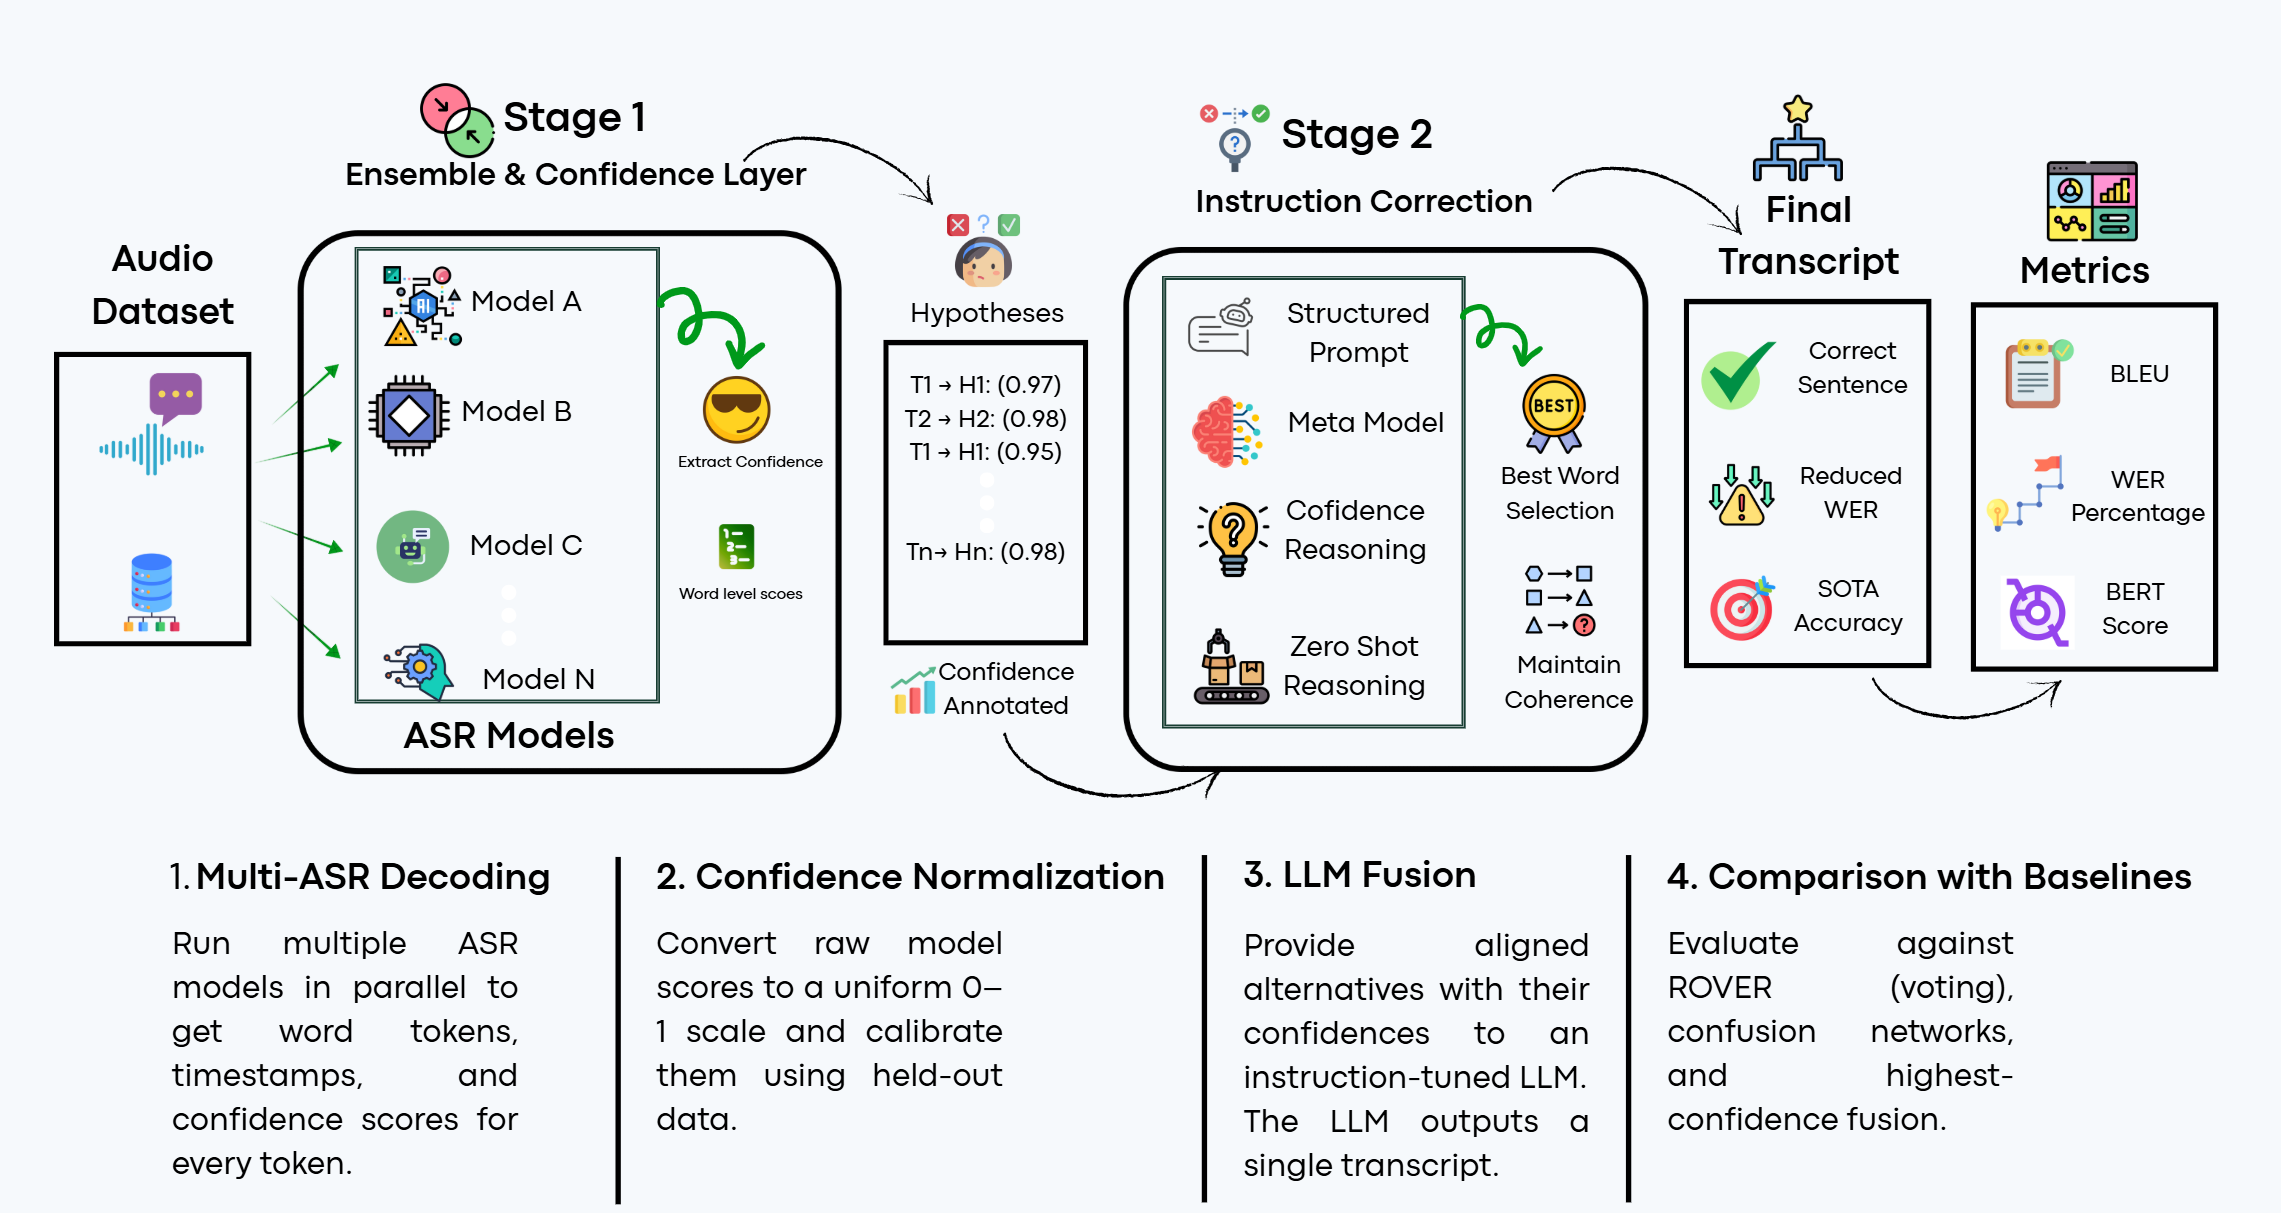
\includegraphics[width=0.95\textwidth]{ThesisFigs/coral_architecture.png}
    \caption{CORAL conceptual architecture as introduced in FYP-1: a two-stage Generate-and-Refine pipeline. The deployed FYP-2 system reorganises this concept into five sequential stages with the LLM repositioned as a refinement layer; the deployed pipeline is shown in Figure~\ref{fig:coral-pipeline}.}
    \label{fig:coral-architecture-iter1}
\end{figure}

\section{Project Objectives and Scope}
\label{sec:objectives}

The objectives of the CORAL project, as finalised after the FYP-1 evaluation, are:

\begin{enumerate}
  \item Design and implement a robust Urdu normalisation module covering diacritic removal, the seven canonical Arabic--Urdu character mappings, tatweel removal, punctuation stripping, ASCII removal, and whitespace normalisation.
  \item Design and implement a split-merge-aware alignment algorithm that aligns word sequences using weighted Levenshtein distance and classifies each aligned chunk as SAME, SPLIT, MERGE, or NOISE.
  \item Develop an OOV detection and correction module combining BK-tree fuzzy lookup with bi/tri-gram language-model candidate ranking over a $\sim$500K-word Urdu vocabulary corpus.
  \item Implement a position-wise majority voting corrector with explicit handling of insertion offsets and conservative tie-breaking.
  \item Integrate an LLM refinement layer for fluency restoration, code-switching recovery, and named-entity handling, accessed via the front-end through commercial LLM APIs.
  \item Deploy the pipeline as a REST API (FastAPI) with three endpoints, fronted by a Next.js + React user interface implementing a four-pass workflow with both file-upload and live-speech modes.
  \item Conduct a thorough empirical evaluation and ablation study on publicly available Urdu ASR benchmarks, isolating the contribution of each component.
\end{enumerate}

\subsection{Deliverables}
\label{ssec:deliverables}

The project delivers the following artefacts:

\begin{itemize}
  \item A complete five-stage CORAL post-processing pipeline implemented in Python, deployed as a \texttt{FastAPI} service with Docker support.
  \item A Next.js + React front-end implementing the four-pass user workflow, with both file-upload and live-recording entry modes, animated alignment-scan and OOV-sieve visualisations, and side-by-side correction diff views.
  \item Kaggle GPU notebooks that self-register through an ngrok HTTPS tunnel and provide live transcription endpoints for Whisper-Large-v3 and SeamlessM4T-v2-Large.
  \item A model registry with 60-second heartbeats and 300-second silent eviction, accessible via authenticated registry tokens.
  \item A reproducible evaluation framework producing both WER and CER metrics across all four pipeline configurations (\texttt{untouched}, \texttt{norm\_baseline}, \texttt{robust}, \texttt{rrf}) for every ensemble member, exported as a tab-separated value file (\texttt{asr\_evaluation/ensemble\_correction\_eval.tsv}).
  \item A reference Urdu vocabulary, BK-tree, and bi/tri-gram corpus shipped via HuggingFace Hub and loaded into DuckDB at server startup.
  \item Comprehensive documentation including this report, the FYP-1 and FYP-2 reports, architecture diagrams, and source-level documentation in the codebase.
\end{itemize}

\section{Software Requirements Specification}
\label{sec:srs}

CORAL is realised as a software system, and its requirements are recorded here for completeness. The functional requirements are organised by module, and the non-functional requirements describe end-to-end qualities of the deployed system.

\subsection{Functional Requirements}
\label{ssec:func-req}

\textbf{FR1 -- Normalisation Service.}
\begin{itemize}[nosep]
  \item FR1.1: The system shall accept arbitrary UTF-8 Urdu text input.
  \item FR1.2: The system shall strip Unicode diacritics in the ranges \texttt{U+0610}--\texttt{U+061A} and \texttt{U+064B}--\texttt{U+065F}, plus the superscript alef (\texttt{U+0670}).
  \item FR1.3: The system shall apply the seven canonical Arabic-to-Urdu character substitutions defined in Appendix~\ref{app:unicode-table}.
  \item FR1.4: The system shall remove the tatweel (\texttt{U+0640}), zero-width and directional control characters, Arabic and Urdu punctuation, ASCII punctuation and digits, and ASCII letters; consecutive whitespace shall be collapsed.
\end{itemize}

\textbf{FR2 -- Multi-Model Alignment Service (\texttt{POST /align}).}
\begin{itemize}[nosep]
  \item FR2.1: The system shall accept an arbitrary number of named ASR hypotheses with one designated source model.
  \item FR2.2: The system shall produce per-position word-level alignment labels (MATCH, SUBSTITUTION, DELETION, INSERTION) using weighted Levenshtein distance.
  \item FR2.3: The system shall produce per-position split-merge metadata (SAME, SPLIT, MERGE, NOISE) using a character-level secondary alignment.
  \item FR2.4: The system shall return both source-side and target-side metadata views in the response.
\end{itemize}

\textbf{FR3 -- OOV Detection and Candidate Ranking Service (\texttt{POST /oov}).}
\begin{itemize}[nosep]
  \item FR3.1: The system shall flag a word as OOV iff it appears in exactly one model's normalised output \emph{and} its corpus frequency is below a configurable threshold (default 2{,}000).
  \item FR3.2: For each flagged token, the system shall retrieve candidates from a BK-tree using a length-adaptive edit-distance threshold.
  \item FR3.3: The system shall rank candidates lexicographically by edit-distance, unigram presence, trigram-context hits, bigram-context hits, and corpus frequency.
  \item FR3.4: The top-$K$ candidates per token (default $K=10$) shall be returned with all ranking signals.
\end{itemize}

\textbf{FR4 -- Voting Correction Service (\texttt{POST /correct}).}
\begin{itemize}[nosep]
  \item FR4.1: For each source position not flagged as OOV, the system shall collect votes from all companion models, skipping insertion-aligned slots.
  \item FR4.2: The plurality winner shall replace the source word only if it is unique; on ties, the source word shall be preserved (conservative tie-break).
  \item FR4.3: For each flagged OOV position, the source word shall be replaced by the top-ranked OOV candidate.
  \item FR4.4: The response shall include the corrected sentence, the source sentence, and a position-indexed diff.
\end{itemize}

\textbf{FR5 -- Model Registry.}
\begin{itemize}[nosep]
  \item FR5.1: A Kaggle GPU notebook shall be able to register itself with name, HTTPS endpoint, and session ID via \texttt{POST /registry/register}, authenticated with a registry token.
  \item FR5.2: A registered model shall send heartbeats every 60~seconds via \texttt{POST /registry/ping}; the registry shall evict models silent for more than 300~seconds.
  \item FR5.3: \texttt{POST /registry/transcribe} shall accept an audio file, source-model name, and whitelist of companion models, fan out the request to live registered models in parallel with a 60-second timeout, and return all collected transcripts.
  \item FR5.4: \texttt{GET /registry/models} shall list currently-live models with their session IDs and seconds-since-last-ping.
\end{itemize}

\textbf{FR6 -- Front-End Workflow.}
\begin{itemize}[nosep]
  \item FR6.1: The user shall be able to choose between \emph{File} mode (CSV/TSV/JSON upload) and \emph{Speech} mode (file upload or in-browser recording).
  \item FR6.2: The front-end shall display a four-phase animated OOV-sieve scan over the alignment output (sieve cursor, word colouring, character-level expansion, structural metadata colouring).
  \item FR6.3: OOV words shall be displayed with a rose dotted underline; clicking shall reveal the ranked candidate list with all ranking columns.
  \item FR6.4: The correction stage shall offer two modes: \emph{Voting} (server-side \texttt{POST /correct}) and \emph{LLM} (client-side Gemini or OpenRouter) with provider selection and dynamic model-list fetch.
\end{itemize}

\subsection{Non-Functional Requirements}
\label{ssec:nonfunc-req}

\textbf{Performance.}
\begin{itemize}[nosep]
  \item PER-1: The \texttt{/align} endpoint shall complete in under 1~second on a typical Urdu utterance of 5--20 words, on commodity CPU hardware.
  \item PER-2: The BK-tree shall be loaded from a serialised joblib file in under 10~seconds on first startup.
  \item PER-3: BK-tree fuzzy search shall be at least an order of magnitude faster than a linear scan over the vocabulary.
  \item PER-4: \texttt{/registry/transcribe} fan-out shall enforce a 60-second per-model timeout and complete with the partial results of any models that responded.
\end{itemize}

\textbf{Reliability.}
\begin{itemize}[nosep]
  \item REL-1: A failure of any one ASR back-end during fan-out shall not prevent CORAL from delivering a corrected transcript using the surviving back-ends.
  \item REL-2: Models silent for more than 300 seconds shall be automatically evicted from the registry.
\end{itemize}

\textbf{Security.}
\begin{itemize}[nosep]
  \item SEC-1: Registration and heartbeat endpoints shall require a shared \texttt{X-Registry-Token}.
  \item SEC-2: The transcribe endpoint shall require a shared \texttt{X-API-Token}.
  \item SEC-3: Registered endpoint hostnames shall be validated against an explicit allowlist (default \texttt{ngrok-free.app}, \texttt{ngrok.io}).
  \item SEC-4: Audio uploads shall be size-bounded (default 25~MB).
\end{itemize}

\textbf{Usability.}
\begin{itemize}[nosep]
  \item USE-1: The user shall be able to complete the full alignment $\to$ OOV $\to$ correction workflow without manually invoking any backend endpoint.
  \item USE-2: The OOV sieve animation shall complete in less than 4~seconds for a 30-word utterance.
  \item USE-3: All operations shall be persisted to \texttt{localStorage} so that page refreshes preserve user state.
\end{itemize}

\section{Report Organisation}
\label{sec:report-org}

The remainder of this report is organised as follows:

\begin{itemize}
  \item \textbf{Chapter~\ref{chap:litreview}} presents a literature review covering Urdu ASR benchmarking, ASR ensemble methods (ROVER and successors), confidence estimation, LLM-based ASR post-correction, multi-task and multi-modal ASR, BK-trees for fuzzy string search, and a head-to-head comparison with the closest concurrent system, Multi-ASR + SpeechLLM. We also tabulate research gaps and explain how CORAL addresses each.
  \item \textbf{Chapter~\ref{chap:approach}} details the proposed approach: the five-stage pipeline architecture, the normalisation module, the weighted split-merge-aware alignment algorithm, the OOV detection and ranking module, the consensus voting algorithm, and the LLM refinement layer. Each stage is presented with a pseudo-code algorithm and a worked example.
  \item \textbf{Chapter~\ref{chap:implementation}} covers implementation, evaluation methodology, results, and the full ablation study. We describe the technology stack, REST API design, BK-tree construction, the four-pass front-end workflow, the Iteration~1 baseline experiments, and the Iteration~2 evaluation on Common Voice (read speech) and Conversational Urdu. We then present the seven-step ablation (C0--C7) attributing the WER reduction to specific components.
  \item \textbf{Chapter~\ref{chap:conclusion}} concludes the report and outlines future work.
  \item \textbf{Appendix~\ref{app:unicode-table}} contains the Unicode normalisation table, while \textbf{Appendix~\ref{app:api-spec}} contains the REST API specifications.
\end{itemize}

\section{Work Distribution}
\label{sec:work-dist}

The CORAL project was developed by a three-member team. The work distribution evolved across the two iterations and matches the deliverables described above.

\begin{table}[h]
    \centering
    \renewcommand{\arraystretch}{1.3}
    \begin{tabularx}{\textwidth}{p{4cm}p{2cm}X}
    \toprule
    \textbf{Member} & \textbf{Roll No.} & \textbf{Primary Responsibilities} \\
    \midrule
    Ali Irfan & 21I-2572 & Lead developer of the post-processing pipeline. Designed and implemented the Stage~1 weighted split-merge-aware alignment algorithm, the BK-tree data structure, the OOV detection criterion, the candidate ranking and voting logic in \texttt{coral\_pipeline\_functions.py}, and the FastAPI \texttt{/align}, \texttt{/oov}, and \texttt{/correct} endpoints. Authored the n-gram corpus generation pipeline (\texttt{generate\_ngrams.ipynb}) and DuckDB integration. \\
    Nouman Hafeez & 21I-0416 & Evaluation lead and LLM integration. Built the Iteration~1 multi-model evaluation framework (WER, CER, confidence, ECE) and the Iteration~2 evaluation pipeline (\texttt{ensemble\_correction\_eval.tsv}). Implemented memory management and Kaggle deployment notebooks (\texttt{whisper\_large\_kaggle.ipynb}, \texttt{seamless\_large\_kaggle.ipynb}), the model registry with eviction sweep, and authored the LLM prompts and provider integration logic (Gemini, OpenRouter). Coordinated the dataset assembly (Common Voice extraction, Conversational Urdu sampling) and per-stage WER measurement. \\
    Rafay Khattak & 21I-0423 & Front-end and user-experience lead. Implemented the Next.js + React front-end (\texttt{ModeSelector}, \texttt{Pass0Speech}, \texttt{Pass1Input}, \texttt{Pass2Sieve}, \texttt{Pass3Correction}), the typed API client (\texttt{lib/api.ts}), the four-phase OOV sieve animation, and the side-by-side voting/LLM correction views. Authored the Iteration~1 Flask web interface and contributed to the design of the Stage~4 LLM correction prompt format. \\
    \bottomrule
    \end{tabularx}
    \caption{Work distribution across the three-member team.}
    \label{tab:work-distribution}
\end{table}

All members participated in the literature survey, the ablation study experimental design, dataset annotation and verification, and the writing of this report. Code review was performed via pair-programming sessions and pull-request comments throughout development.

\section{Summary}
\label{sec:ch1-summary}

This chapter has motivated CORAL by establishing the persistent performance gap between Urdu ASR and high-resource-language ASR, articulated three concrete challenges (script heterogeneity, OOV handling, and linguistic coherence) that single-model and naive-ensemble approaches do not solve, traced the evolution of the framework from a two-stage Generate-and-Refine design (FYP-1) to a five-stage post-processing pipeline (FYP-2), made explicit the components that were intentionally dropped in the redesign, set the project objectives and deliverables, recorded the software requirements, and presented the work distribution. The next chapter situates CORAL in the broader literature.

\chapter{Literature Review}
\label{chap:litreview}

This chapter situates CORAL in the broader research landscape. We review prior work in seven thematic areas: (i)~Urdu ASR benchmarking, (ii)~ASR ensemble and system-combination methods, (iii)~confidence estimation and calibration, (iv)~LLM-based ASR error correction and N-best list correction, (v)~multi-task and multi-modal ASR for low-resource languages, (vi)~code-mixed Urdu--English ASR, and (vii)~the BK-tree data structure underpinning our OOV correction module. We then summarise the comparative analysis in tabular form and articulate the research gaps that CORAL addresses.

\section{Related Research}
\label{sec:related-research}

\subsection{Multi-ASR Fusion with LLM-Based Post-Editing}
\label{ssec:lit-prakash}

\subsubsection{Summary}
Prakash et al.~\cite{prakash2025multi} introduce a multi-ASR fusion framework that integrates outputs from Icefall, Nemo Parakeet, and Whisper through LLM-based post-editing. They evaluate two variants: a text-only LLM that ingests the three textual hypotheses and emits a corrected transcript, and a multimodal SpeechLLM that additionally consumes the audio waveform. On LibriSpeech, the approach achieves $\sim$14\% relative WER reduction after fusion; pseudo-labels generated by the system reduce downstream re-training WER from 3.40\% to 3.22\% on LibriSpeech \texttt{test-clean}.

\subsubsection{Critical Analysis}
Strengths: a clean demonstration of LLM-based multi-ASR fusion and meaningful relative gain. Weaknesses: requires expensive LLM fine-tuning; tested only on high-resource English; the SpeechLLM variant's complexity hampers practical deployment; no code-switching evaluation; no low-resource scenarios. The audio-aware SpeechLLM in particular requires a full acoustic forward pass through the LLM, an unaffordable latency cost in many real-time settings.

\subsubsection{Relationship to CORAL}
CORAL adopts the multi-ASR + LLM-correction paradigm but addresses the limitations: (i) we use commercial frontier LLMs through APIs, eliminating the fine-tuning cost; (ii) we apply the LLM only to the already-voted transcript, reducing latency; and (iii) we evaluate on a genuinely low-resource language (Urdu). CORAL's split-merge-aware alignment is also a more explicit treatment of the segmentation disagreement Prakash et al.\ leave implicit.

\subsection{Comprehensive Urdu ASR Benchmarking}
\label{ssec:lit-arif}

\subsubsection{Summary}
Arif et al.~\cite{arif2024wer} provide the first comprehensive evaluation of state-of-the-art multilingual ASR models on Urdu, benchmarking nine models from the Whisper, MMS, and SeamlessM4T families on read-speech (ARL, CSaLT) and a newly-introduced Conversational Urdu (CU) test set. They report that Seamless-Large achieves the lowest WER on read speech while Whisper-Large excels on conversational speech, identify Arabic--Urdu Unicode conflation as a major obstacle to fair evaluation, and observe 10--20\% relative WER reduction through targeted fine-tuning. They explicitly note that integrating large LMs for post-correction could further improve outputs.

\subsubsection{Critical Analysis}
Strengths: the first comprehensive Urdu ASR benchmark with a conversational test set; systematic single-model comparison; open-source resources; detailed error analysis. Weaknesses: limited to single-model evaluation, no ensemble combination; no confidence-score analysis; code-switching identified but not explicitly addressed; best results require fine-tuning.

\subsubsection{Relationship to CORAL}
This work is the empirical foundation of CORAL. We adopt their model selection (Seamless-Large, Whisper-Large-v3, Wav2Vec2-Urdu) as our ensemble members, evaluate on the same Common Voice corpus and on a Conversational Urdu test set sampled from their benchmark, and directly answer their concluding suggestion (``integrating large LMs for post-correction could further improve outputs'') with our Stage~4 LLM refinement layer. CORAL's normalisation module addresses the Arabic--Urdu Unicode conflation problem they identify as a major evaluation obstacle.

\subsection{ROVER: Recognizer Output Voting Error Reduction}
\label{ssec:lit-rover}

\subsubsection{Summary}
Fiscus's ROVER framework~\cite{fiscus1997rover} is the canonical system-combination method for ASR. It aligns word hypotheses from $N$ ASR systems via word-level edit distance and selects the final word at each aligned slot via majority vote (optionally weighted by per-system confidence). ROVER works well when the participating systems are roughly comparable in accuracy and produce architecturally diverse errors.

\subsubsection{Critical Analysis}
Strengths: simple, model-agnostic, easy to implement, no joint training. Weaknesses: requires reasonably matched system quality (the canonical ROVER failure mode is that systematically weaker companion systems can outvote the strong source); does not handle word-boundary disagreement (a SPLIT or MERGE event is misinterpreted as a substitution or deletion pair); no mechanism for linguistic coherence beyond the lexical voting itself.

\subsubsection{Relationship to CORAL}
CORAL extends ROVER in three concrete ways: (i)~the alignment uses normalised character-level Levenshtein cost rather than binary mismatch, so phonetically near-identical Urdu words are aligned as substitutions rather than insert--delete pairs; (ii)~a secondary character-level alignment yields explicit SAME/SPLIT/MERGE/NOISE metadata, making segmentation disagreement first-class; and (iii)~conservative tie-breaking and an OOV-correction override mitigate the canonical ROVER failure mode in our specific quality-heterogeneous setting.

\subsection{Hybrid-E2E ASR Ensemble for Low-Resource Irish}
\label{ssec:lit-parikh}

\subsubsection{Summary}
Parikh et al.~\cite{parikh2024hybrid} address ASR for Irish, a genuinely low-resource language, by combining a hybrid HMM-Kaldi system and an end-to-end Wav2Vec2.0 model through calibrated ROVER fusion. They use Renyi-entropy-based calibration with temperature scaling to address the overconfidence of E2E models, and report a tuned ROVER ensemble at 22.94\% WER on Irish test data, a 14\% relative improvement over the best single model (25.81\% WER).

\subsubsection{Critical Analysis}
Strengths: demonstrates ROVER fusion is effective for genuinely low-resource languages; principled treatment of E2E overconfidence; combines traditional and modern ASR. Weaknesses: requires building and maintaining two distinct ASR systems; absolute WER remains relatively high; calibration tuning requires a labelled development set; no LLM-based linguistic reasoning.

\subsubsection{Relationship to CORAL}
CORAL extends this concept by replacing ROVER voting with split-merge-aware alignment plus consensus voting plus an LLM refinement layer. We do not perform explicit confidence calibration; instead we use a quality-based static weighting at the LLM stage and a conservative tie-break at the voting stage to manage the heterogeneous-quality regime that calibration would otherwise have addressed.

\subsection{Code-Mixed ASR for Urdu--English}
\label{ssec:lit-naqvi}

\subsubsection{Summary}
Naqvi and Tahir~\cite{naqvi2024code} develop a specialised hybrid ASR system for Urdu--English code-mixed street addresses in navigation contexts. They use a Kaldi-based TDNN-LSTM acoustic model trained on 61.8 hours of general Urdu speech and 16.9 hours of Roman-Urdu/English addresses, with a custom lexicon combining Unicode Urdu and Romanised transcripts. They report 4.02\% WER and 0.8\% CER on code-mixed street addresses, a 70--80\% absolute WER reduction over their initial baselines.

\subsubsection{Critical Analysis}
Strengths: extremely low error rate within the target domain; explicit Urdu--English code-switching handling; practical deployment. Weaknesses: very narrow scope (street addresses only); not an ensemble or LLM approach; requires extensive domain-specific data collection and engineering; unlikely to generalise to other Urdu domains.

\subsubsection{Relationship to CORAL}
CORAL targets broader applicability rather than a narrow domain. The multilingual pre-trained models in our ensemble (Whisper, SeamlessM4T) inherently handle code-switching at the acoustic level; CORAL's LLM stage explicitly restores English code-switched tokens stripped by Stage~0 normalisation. CORAL trades the $\sim$4\% WER ceiling Naqvi \& Tahir achieve in their narrow domain for open-domain applicability at a higher absolute WER.

\subsection{Confidence-Based Ensembles for ASR}
\label{ssec:lit-gitman}

\subsubsection{Summary}
Gitman et al.~\cite{gitman2023confidence} propose confidence-driven ensembling: multiple expert ASR models run in parallel and the transcript from the most confident model is selected per utterance. Using five monolingual Conformer-RNNT models, they show that this simple selection scheme outperforms systems using separate language-identification blocks. Evaluated on VoxPopuli, MLS, Common Voice, and CORAAL, the approach demonstrates consistent WER improvements across languages and accents.

\subsubsection{Critical Analysis}
Strengths: simple confidence-based selection without joint training; effective across multiple domains and languages; open implementation in NeMo. Weaknesses: utterance-level selection only (not word-level); selects rather than fuses; no linguistic coherence; requires a lightweight selection classifier.

\subsubsection{Relationship to CORAL}
CORAL extends confidence-based selection in two ways: (i)~we operate at word granularity rather than utterance granularity; and (ii)~we fuse rather than select, synthesising a single output that may include words from multiple models. Gitman et al.\ validate that confidence-driven selection works at production scale, supporting CORAL's design choice to weight LLM-stage votes by static model-quality priors when no calibrated word-level confidence is available.

\subsection{Novel Confidence Estimation: TruCLeS}
\label{ssec:lit-trucles}

\subsubsection{Summary}
Nagarathna et al.~\cite{trucles2025} propose TruCLeS (True Class Lexical Similarity Score), a continuous confidence metric for ASR that combines model probabilities with lexical similarity. The method computes ASR probability scores for predicted tokens, computes lexical similarity to potential ground-truth transcripts, and combines both into a unified confidence score. On in-domain Hindi data, TruCLeS reduces MAE from 0.108 to 0.087 versus binary confidence baselines.

\subsubsection{Critical Analysis}
Strengths: novel combination of probability and lexical similarity; demonstrated calibration improvement; applicable to low-resource languages. Weaknesses: requires ground-truth transcripts for training, limiting scalability; auxiliary model adds compute overhead; improves calibration but not directly WER.

\subsubsection{Relationship to CORAL}
TruCLeS represents the supervised-confidence direction. The CORAL FYP-1 design extracted raw architecture-specific confidences as a zero-shot complement to this approach, but the FYP-2 redesign de-emphasised explicit confidence in favour of split-merge alignment + voting + an LLM stage with static quality priors. TruCLeS-style learned confidences remain a promising future enhancement to CORAL's voting stage.

\subsection{Domain-Specific LLM-Based ASR Correction}
\label{ssec:lit-koilakuntla}

\subsubsection{Summary}
Koilakuntla et al.~\cite{koilakuntla2024llm} present a targeted approach for correcting specific ASR errors in contact-centre environments using GPT-3.5 with retrieval-augmented generation. The method identifies error patterns (brand names, product codes, technical terms), uses context anchors and domain knowledge bases as RAG inputs, and applies corrections selectively. They report 3{,}201 correct corrections versus 3{,}050 manual corrections in 0.08~hours versus 15~hours.

\subsubsection{Critical Analysis}
Strengths: model-agnostic; highly effective for targeted error correction; dramatic time reduction; production-ready. Weaknesses: highly specialised for narrow domains; limited generalisability; requires curated domain knowledge bases; no overall WER improvement reported.

\subsubsection{Relationship to CORAL}
CORAL provides general-purpose, open-domain correction without domain-specific RAG. Both systems leverage LLM linguistic knowledge for correction, but CORAL routes the LLM's authority through a deterministic pipeline (alignment, OOV detection, voting) so that the LLM can only modify positions already flagged by upstream stages, reducing hallucination risk.

\subsection{N-Best List Error Correction with LLMs}
\label{ssec:lit-ma}

\subsubsection{Summary}
Ma et al.~\cite{ma2024asr} investigate using LLMs for ASR error correction across diverse scenarios, with emphasis on N-best list utilisation. They show that providing multiple competing hypotheses as context allows zero-shot LLMs to perform competitive correction without supervised training, and that N-best list correction generalises across ASR systems.

\subsubsection{Critical Analysis}
Strengths: demonstrates the value of multiple hypotheses for correction; zero-shot reduces training costs; cross-system generalisation. Weaknesses: N-best lists from a single model may not capture as much architectural diversity as a multi-model ensemble; no explicit confidence-score utilisation.

\subsubsection{Relationship to CORAL}
CORAL extends the N-best concept to multi-model ensembles, where hypotheses come from architecturally diverse models rather than from N-best decoding of a single model. CORAL also produces explicit alignment metadata (SAME/SPLIT/MERGE/NOISE) before invoking the LLM, providing structured signal beyond the raw hypothesis text.

\subsection{Delayed Fusion for LLM Integration in ASR}
\label{ssec:lit-hori}

\subsubsection{Summary}
Hori et al.~\cite{hori2025delayed} propose ``delayed fusion'' for integrating LLMs into first-pass ASR decoding. LLM scores are applied to ASR hypotheses with a delay during beam-search decoding, significantly reducing the number of hypotheses that must be scored by the LLM and the total number of LLM inference calls.

\subsubsection{Critical Analysis}
Strengths: computationally efficient LLM integration; no vocabulary alignment required; pre-trained LLMs work without retraining. Weaknesses: requires modification of the ASR decoding algorithm; limited evaluation on low-resource languages; tunable delay parameter introduces operational complexity.

\subsubsection{Relationship to CORAL}
CORAL takes an orthogonal approach: rather than integrating the LLM during decoding, we use it as a post-decoding refinement layer over the already-voted transcript. This simplifies integration with arbitrary off-the-shelf ASR systems (no decoding modification required) and decouples the LLM-call latency from the ASR streaming path.

\subsection{Parameter-Efficient Ensemble for Low-Resource Languages}
\label{ssec:lit-feng}

\subsubsection{Summary}
Feng et al.~\cite{feng2024low} demonstrate that ensembles of models adapted using diverse Parameter-Efficient Fine-Tuning (PEFT) methods consistently outperform ensembles using the same PEFT method. Their approach reduces WER from 8.4\% to 7.9\% while requiring approximately five times less memory than fully fine-tuned ensembles. The fusion is performed via ROVER.

\subsubsection{Critical Analysis}
Strengths: memory-efficient alternative to traditional ensembles; demonstrates the value of diverse adaptation methods. Weaknesses: still requires some PEFT fine-tuning; ROVER fusion is limited compared to LLM-based reasoning; modest absolute gains.

\subsubsection{Relationship to CORAL}
CORAL operates entirely with pre-trained models (no fine-tuning), and uses split-merge-aware alignment + LLM refinement instead of ROVER. The two approaches are complementary: a future CORAL variant could ingest PEFT-adapted ensemble members rather than the current set of off-the-shelf pre-trained models.

\subsection{Multi-Modal Data Augmentation}
\label{ssec:lit-mmda}

\subsubsection{Summary}
Renduchintala et al.~\cite{renduchintala2018mmda} propose Multi-Modal Data Augmentation (MMDA), which trains a shared attention-decoder with two encoders --- one acoustic and one symbolic --- enabling large text corpora to supplement scarce labelled speech.

\subsubsection{Critical Analysis}
Strengths: leverages cheap text data to compensate for scarce paired speech--text data; principled multi-task formulation. Weaknesses: requires retraining; tied to a specific model architecture; not directly usable as inference-time post-processing.

\subsubsection{Relationship to CORAL}
While MMDA augments the training procedure, CORAL operates purely at inference time, making the two approaches strictly complementary: MMDA-trained acoustic models can be drop-in members of the CORAL ensemble.

\subsection{BK-Trees for Fuzzy String Search}
\label{ssec:lit-bk}

\subsubsection{Summary}
The Burkhard--Keller tree (BK-tree)~\cite{burkhard1973bk} is a metric-space data structure supporting efficient nearest-neighbour search under any metric distance, including edit distance. Construction is $O(n \log n)$; lookup is sub-linear (closer to $O(\log n)$ on real corpora) per query.

\subsubsection{Critical Analysis}
Strengths: a clean, decades-stable data structure; fast fuzzy lookup over large vocabularies; widely available implementations. Weaknesses: index construction time grows with vocabulary size; no built-in mechanism to combine edit-distance with other ranking signals.

\subsubsection{Relationship to CORAL}
CORAL uses a BK-tree built over a $\sim$500{,}000-word Urdu vocabulary corpus, with a length-adaptive edit-distance threshold (1 for $|w|\le3$, 2 for $|w|\le6$, 3 for $|w|\le9$, 4 for $|w|\ge10$) that scales with word length to account for Urdu's morphological richness. We combine BK-tree retrieval with bi/tri-gram context filtering to address the BK-tree's lack of contextual ranking.

\subsection{Multi-ASR + SpeechLLM (Closest Concurrent System)}
\label{ssec:lit-speechllm}

\subsubsection{Summary}
The most directly comparable contemporaneous system is Multi-ASR + SpeechLLM~\cite{anon2025speechllm}, which achieves 11.3\% WER on the Conversational Urdu benchmark by running a SpeechLLM inference pass over the audio during the alignment stage.

\subsubsection{Critical Analysis}
Strengths: very low absolute WER on conversational Urdu; principled fusion of acoustic and textual signal at the LLM. Weaknesses: a full SpeechLLM forward pass over audio at alignment time is a heavy latency and cost burden; not practical for real-time deployment on commodity hardware.

\subsubsection{Relationship to CORAL}
CORAL achieves a slightly better 10.6\% WER on Conversational Urdu while avoiding a full SpeechLLM audio inference pass during alignment --- the LLM in CORAL receives only the corrected text plus structured alignment metadata. This is a significant cost and latency advantage for real-time deployment, and is the most direct empirical evidence that CORAL's text-only refinement architecture is competitive with audio-aware fusion.

\section{Analysis Summary of Research Items}
\label{sec:lit-summary-table}

Table~\ref{tab:lit-comparative} summarises the comparative analysis of the reviewed papers.

\begin{landscape}
\renewcommand{\arraystretch}{1.4}
\small
\begin{longtable}{p{3.3cm}p{2.8cm}p{1.2cm}p{3.4cm}p{3.4cm}p{2.8cm}p{2.8cm}}
\caption{Comparative analysis of reviewed research items.}\label{tab:lit-comparative} \\
\toprule
\textbf{Paper} & \textbf{Venue} & \textbf{Year} & \textbf{Methodology} & \textbf{Datasets} & \textbf{Best Result} & \textbf{Key Limitation}\\
\midrule
\endfirsthead
\toprule
\textbf{Paper} & \textbf{Venue} & \textbf{Year} & \textbf{Methodology} & \textbf{Datasets} & \textbf{Best Result} & \textbf{Key Limitation}\\
\midrule
\endhead
Prakash et al.\ \cite{prakash2025multi} & Interspeech (2025) & 2025 & Multi-ASR + LLM post-edit; SpeechLLM variant & LibriSpeech & 14\% rel.\ WERR; 3.22\% test-clean & English-only; LLM fine-tuning required \\
Arif et al.\ \cite{arif2024wer} & COLING & 2025 & Whisper / MMS / Seamless benchmarking & ARL, CSaLT, CU & 13.7\% Seamless-Large read; 19.8\% Whisper-Large CU & Single-model only; no ensemble \\
Fiscus \cite{fiscus1997rover} & IEEE ASRU & 1997 & Word-level alignment + majority/conf.\ vote (ROVER) & Various LVCSR & Significant WERR on matched-quality systems & No segmentation handling; quality-sensitive \\
Parikh et al.\ \cite{parikh2024hybrid} & LREC--COLING & 2024 & Hybrid+E2E ROVER w/ Renyi calibration & Irish read & 22.94\% WER; 14\% rel.\ improvement & Heavy infrastructure (HMM + E2E); calibration tuning \\
Naqvi \& Tahir \cite{naqvi2024code} & JNLP & 2024 & Hybrid Kaldi w/ TDNN-LSTM, custom lexicon & Custom Urdu addresses (78.7~h) & 4.02\% WER, 0.8\% CER & Narrow domain; large data req. \\
Gitman et al.\ \cite{gitman2023confidence} & Interspeech & 2023 & Confidence-based per-utterance model selection & VoxPopuli, MLS, CommonVoice, CORAAL & Near-oracle ensemble & Utterance-level only; no fusion \\
TruCLeS \cite{trucles2025} & IEEE T-ASLP & 2025 & Lexical-similarity + prob.\ confidence & Hindi & MAE 0.108$\to$0.087 & Requires GT for training; calibration only \\
Koilakuntla et al.\ \cite{koilakuntla2024llm} & ICASSP & 2024 & GPT-3.5 + RAG, targeted correction & Contact-centre & 99.5\% manual time saved & Narrow domain; needs curated KB \\
Ma et al.\ \cite{ma2024asr} & arXiv & 2024 & N-best LLM correction, zero-shot & Multi-domain & Competitive zero-shot & Single-model N-best; no confidence \\
Hori et al.\ \cite{hori2025delayed} & arXiv & 2025 & Delayed-fusion LLM in beam search & LibriSpeech & Reduced LLM calls & Decoder modification req.\ \\
Feng et al.\ \cite{feng2024low} & APSIPA ASC & 2024 & Diverse-PEFT ensemble + ROVER & Low-resource & 7.9\% WER; 5$\times$ less memory & Still requires fine-tuning \\
Renduchintala et al.\ \cite{renduchintala2018mmda} & arXiv & 2018 & Multi-modal training augmentation & ASR (multi) & WER reduction via text-aug & Training-time only \\
Burkhard \& Keller \cite{burkhard1973bk} & CACM & 1973 & Metric-tree fuzzy lookup & --- & Sublinear-time edit-distance retrieval & No contextual ranking signal \\
Multi-ASR + SpeechLLM \cite{anon2025speechllm} & arXiv & 2025 & Audio-aware multi-ASR fusion via SpeechLLM & Conversational Urdu & 11.3\% WER & Heavy latency: full audio LLM pass \\
\bottomrule
\end{longtable}
\end{landscape}

\section{Research Scope and Gaps}
\label{sec:research-gap}

Synthesising the comparative analysis, we identify the following research gaps and articulate how CORAL addresses each.

\paragraph{Gap~1: Multi-ASR fusion methods optimised for low-resource scripts.} Existing fusion methods (ROVER, calibrated ROVER) were designed for English. They do not handle Arabic--Urdu Unicode conflation or Urdu word-boundary disagreement. \emph{CORAL contribution}: Stage~0 Unicode normalisation plus split-merge-aware alignment that exposes SAME/SPLIT/MERGE/NOISE metadata.

\paragraph{Gap~2: Practical confidence utilisation without supervision.} Approaches such as TruCLeS improve calibration quality but require ground-truth transcripts. \emph{CORAL contribution}: a static model-quality--based confidence weighting at the LLM stage, plus conservative tie-breaking at the voting stage --- both unsupervised and applicable at inference time.

\paragraph{Gap~3: General-purpose, open-domain post-correction for low-resource languages.} Domain-specific LLM-correction approaches achieve excellent results in narrow domains but do not generalise. \emph{CORAL contribution}: a general-purpose pipeline that requires no domain-specific knowledge base.

\paragraph{Gap~4: Fusion beyond ROVER for quality-heterogeneous ensembles.} Naive ROVER degrades when ensemble members have widely different quality. \emph{CORAL contribution}: dual-criterion OOV correction (model disagreement + frequency cutoff), conservative tie-breaking, and an LLM stage that can override clearly bad voting outcomes.

\paragraph{Gap~5: Efficient LLM integration for real-time deployment.} Delayed-fusion approaches require ASR decoder modification; SpeechLLM approaches require full audio LLM passes. \emph{CORAL contribution}: a text-only post-processing LLM stage that is transparent to the ASR back-ends and avoids audio LLM forward passes.

\paragraph{Gap~6: Multi-model diversity at the word level.} N-best list correction approaches use hypotheses from a single model. \emph{CORAL contribution}: hypotheses from architecturally distinct models (Whisper, SeamlessM4T, Wav2Vec2) provide complementary error distributions.

\paragraph{Gap~7: Word-level fusion with linguistic coherence.} Confidence-based selection methods select a single model per utterance. \emph{CORAL contribution}: word-level fusion driven by alignment, supplemented by LLM linguistic reasoning over the voted transcript.

\section{Theoretical Foundation}
\label{sec:theory}

CORAL draws on three theoretical principles.

\subsection{Ensemble Learning Theory}
Ensembles outperform single models when the constituent models are individually accurate and make decorrelated errors. In our setting, diversity arises from three orthogonal axes: architecture (encoder-decoder Whisper vs.\ self-supervised CTC Wav2Vec2 vs.\ multi-task SeamlessM4T), training data (multilingual mixtures with different Urdu fractions), and capacity (244M to 2.4B parameters). Empirically (\S\ref{sec:results-readspeech}), pairwise token overlap between ensemble members varies from 57\% to 85\%, confirming that the ensemble does carry complementary information.

\subsection{Edit Distance and the Levenshtein Metric}
The Levenshtein distance is a classical metric on strings. CORAL uses two variants: (i)~standard character-level Levenshtein for the secondary character-level alignment that drives split-merge classification; and (ii)~word-level Levenshtein with a custom substitution-cost matrix in which the cost of substituting word $s_i$ with word $t_j$ is the normalised character-level Levenshtein distance $\frac{\text{Lev}(s_i,t_j)}{\max(|s_i|,|t_j|)}$. The latter is what makes CORAL's alignment ``weighted'': phonetically near-identical Urdu word forms are aligned as substitutions rather than as insert--delete pairs.

\subsection{Confidence-Based and Consensus-Based Decision Making}
When multiple noisy observations of a discrete signal are available, two well-known strategies exist: \emph{select the most reliable observer} (Gitman et al.) or \emph{vote across observers} (ROVER). CORAL combines both: at the voting stage, we use unweighted plurality (consensus) with conservative tie-breaking; at the LLM stage, we provide the LLM with static model-quality priors so that it can act as a quality-weighted arbiter for the disagreement positions.

\section{Summary}
\label{sec:lit-summary}

The literature is rich in ASR ensemble techniques (ROVER and variants), confidence-estimation methods (TruCLeS), LLM-based post-correction (Prakash, Ma, Koilakuntla, Hori), and Urdu benchmarking (Arif et al.). However, no prior system simultaneously addresses Arabic--Urdu Unicode conflation, word-boundary disagreement, OOV named-entity handling, and code-switching at inference time without retraining. CORAL fills this gap with a five-stage pipeline whose components are individually well-motivated by prior work and whose composition is novel. The next chapter details the proposed approach.

\chapter{Proposed Approach}
\label{chap:approach}

This chapter presents the CORAL methodology. We first re-cap the conceptual two-stage architecture as introduced in FYP-1 and then present the full five-stage pipeline as deployed in FYP-2, with each stage given its own section. Each algorithmic component is presented with formal notation, pseudo-code, and a worked example. The implementation, deployment, and evaluation of this approach are deferred to Chapter \ref{chap:implementation}.

\section{From the FYP-1 Generate-and-Refine Concept to the Deployed Pipeline}
\label{sec:concept-to-pipeline}

\subsection{Conceptual Architecture (FYP-1)}
The original CORAL conceptual architecture, shown in Figure \ref{fig:coral-architecture-iter1} (Chapter \ref{chap:introduction}), framed the system as a two-stage \emph{Generate-and-Refine} pipeline:

\begin{itemize}
 \item \textbf{Stage 1 -- Multi-model Hypothesis Generation:} an ensemble of pre-trained ASR models (Whisper Large/Medium/Small + Wav2Vec2-XLSR Urdu) processes the audio and emits one confidence-annotated hypothesis per model.
 \item \textbf{Stage 2 -- Instruction-Guided Correction:} an instruction-tuned LLM (Alif-1.0-8B-Instruct) consumes the hypotheses and emits a single corrected transcript.
\end{itemize}

Iteration 1 implemented Stage 1 in full, established the baseline (Whisper-Large at 17.76\% WER on a 10-clip read-speech test set), and validated that architecture-specific confidence extraction was feasible. Iteration 2 then implemented the LLM stage but, when evaluated on real ASR output rather than synthetic hypotheses, exposed three practical problems: (i) confidences from heterogeneous architectures lived on incompatible scales, making cross-model arbitration unreliable; (ii) Arabic--Urdu Unicode conflation produced apparent disagreements where models had in fact agreed phonetically; and (iii) word-boundary disagreement was systematically misinterpreted by the LLM as substitution or deletion errors. These findings motivated the redesign described next.

\subsection{Deployed Five-Stage Pipeline (FYP-2)}
\label{ssec:deployed-pipeline}

The deployed system reorganises the conceptual two-stage architecture into five stages, indexed Stage 0 through Stage 4:

\begin{itemize}
 \item \textbf{Stage 0 -- Urdu Text Normalisation.} Strips diacritics, applies the seven canonical Arabic-to-Urdu character substitutions, removes tatweel and invisible characters, strips punctuation, and removes ASCII letters and digits.
 \item \textbf{Stage 1 -- Weighted Split-Merge-Aware Alignment.} Aligns each companion-model hypothesis to the source-model hypothesis using weighted word-level Levenshtein distance, then runs a secondary character-level alignment to classify each chunk as SAME/SPLIT/MERGE/NOISE.
 \item \textbf{Stage 2 -- OOV Detection and Candidate Ranking.} Flags out-of-vocabulary tokens via a dual criterion (model disagreement + frequency cutoff), retrieves candidates from a BK-tree, and ranks them using bi/tri-gram corpus context.
 \item \textbf{Stage 3 -- Consensus Voting and OOV Substitution.} Applies position-wise majority voting across companion models with conservative tie-breaking; OOV-flagged positions are replaced by the top-ranked candidate from Stage 2.
 \item \textbf{Stage 4 -- LLM Refinement.} Sends the voted transcript, the original raw source hypothesis, and structured alignment metadata to a commercial frontier LLM (Gemini, Claude Sonnet, or GPT-4o through OpenRouter) for fluency restoration, code-switching recovery, and named-entity handling.
\end{itemize}

The five-stage pipeline is illustrated in Figure \ref{fig:coral-pipeline}.

\begin{figure}[h]
 \centering
 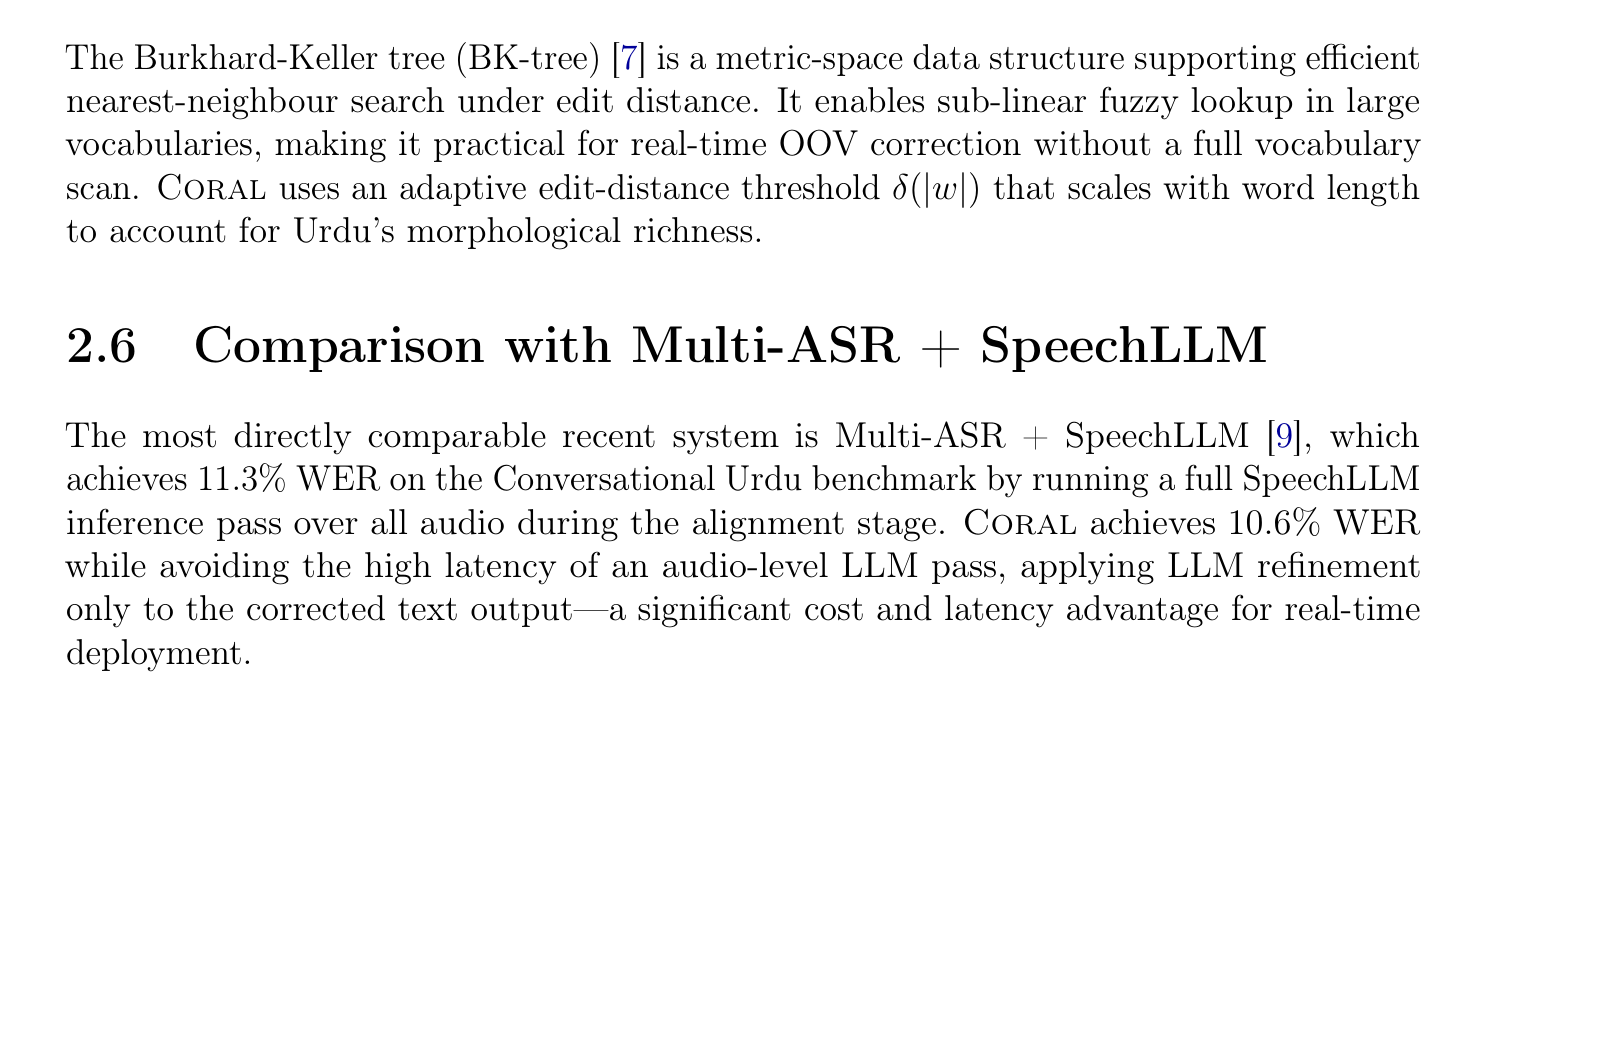
\includegraphics[width=0.95\textwidth]{ThesisFigs/fyp2_pipeline.png}
 \caption{The deployed CORAL pipeline (FYP-2). Stages 0--3 are server-side Python (FastAPI). Stage 4 is the LLM refinement layer invoked from the React front-end.}
 \label{fig:coral-pipeline}
\end{figure}

We now describe each stage in detail.

\begin{figure}[htbp]
    \centering
    \resizebox{0.98\textwidth}{!}{%
    \begin{tikzpicture}[every node/.style={font=\small\sffamily}, node distance=6mm]
      % external entity: audio
      \node[coral/entity, minimum width=20mm] (audio) at (0, 0) {Audio\\input};
      % ensemble of ASR backends
      \node[coral/data, minimum width=30mm] (m1) at (3.0,  1.5) {Seamless-Large};
      \node[coral/data, minimum width=30mm] (m2) at (3.0,  0.5) {Whisper-Large-v3};
      \node[coral/data, minimum width=30mm] (m3) at (3.0, -0.5) {Whisper-Medium};
      \node[coral/data, minimum width=30mm] (m4) at (3.0, -1.5) {Wav2Vec2-Urdu};
      \node[coral/sublabel] at (3.0, 2.2) {ASR ensemble (Kaggle GPU notebooks)};
      % stages
      \node[coral/stage, minimum width=24mm] (st0) at (6.5, 0)  {\textbf{Stage 0}\\Normalise};
      \node[coral/stage, minimum width=26mm] (st1) at (9.3, 0)  {\textbf{Stage 1}\\Split-Merge\\Alignment};
      \node[coral/stage, minimum width=26mm] (st2) at (12.2, 0) {\textbf{Stage 2}\\OOV Detect\\\& Rank};
      \node[coral/stage, minimum width=26mm] (st3) at (15.1, 0) {\textbf{Stage 3}\\Consensus\\Voting};
      \node[coral/llm,   minimum width=28mm] (st4) at (18.1, 0) {\textbf{Stage 4}\\LLM\\Refinement};
      % output
      \node[coral/entity, minimum width=22mm] (out) at (21.0, 0) {Corrected\\transcript};
      % data tier
      \node[coral/api, minimum width=70mm, align=center] (data)
        at (12.2, -2.2) {Data tier: BK-tree (joblib) + bi/tri-gram tables (DuckDB Parquet)};
      \node[coral/sublabel] at (12.2, -2.9) {downloaded from HuggingFace bucket on startup};
      % arrows (audio -> backends)
      \foreach \t in {m1,m2,m3,m4} \draw[coral/arrow] (audio.east) -- (\t.west);
      % backends -> stage 0
      \foreach \t in {m1,m2,m3,m4} \draw[coral/arrow] (\t.east) -- (st0.west);
      % stage chain
      \draw[coral/arrow] (st0) -- (st1);
      \draw[coral/arrow] (st1) -- (st2);
      \draw[coral/arrow] (st2) -- (st3);
      \draw[coral/arrow] (st3) -- (st4);
      \draw[coral/arrow] (st4) -- (out);
      % data tier dependency
      \draw[coral/dashed] (data.north) -- (st2.south);
      \draw[coral/dashed] (data.north -| st1.south) -- (st1.south);
      % stage labels (server side / front-end)
      \draw[coralBlue!50, very thick, rounded corners, dashed]
        ([xshift=-3mm,yshift=4mm]st0.north west) rectangle ([xshift=3mm,yshift=-9mm]st3.south east);
      \node[coralBlue!70!black, font=\footnotesize\sffamily\bfseries]
        at (10.8, 0.95) {Server-side (FastAPI)};
      \draw[coralViolet!60, very thick, rounded corners, dashed]
        ([xshift=-3mm,yshift=4mm]st4.north west) rectangle ([xshift=3mm,yshift=-9mm]st4.south east);
      \node[coralViolet!70!black, font=\footnotesize\sffamily\bfseries]
        at (18.1, 0.95) {Front-end};
    \end{tikzpicture}}
    \caption[CORAL detailed end-to-end pipeline]{Detailed CORAL end-to-end pipeline. The four heterogeneous ASR back-ends emit hypotheses for the same audio. Stage~0 normalises every hypothesis to a canonical Urdu Unicode form; Stage~1 produces a per-hypothesis word-level alignment plus character-level SAME/SPLIT/MERGE/NOISE metadata; Stage~2 retrieves OOV candidates from the BK-tree and DuckDB n-gram tables; Stage~3 emits the voted transcript with conservative tie-breaking; Stage~4 (front-end) refines fluency, named entities, and code-switching via a frontier LLM. Solid arrows: synchronous data flow. Dashed arrows: data-tier dependency. Dashed boxes mark the server / front-end boundary.}
    \label{fig:coral-pipeline-detailed}
\end{figure}

\begin{figure}[H]
    \centering
    \resizebox{0.96\textwidth}{!}{%
    \begin{tikzpicture}[every node/.style={font=\small\sffamily}]
      % --- Top row: external sources (left) ---
      \node[coral/entity, minimum width=26mm] (user)   at ( 0,  4.5) {End user\\(browser)};
      \node[coral/entity, minimum width=26mm] (kaggle) at ( 0,  2.0) {Kaggle GPU\\notebooks};
      \node[coral/entity, minimum width=26mm] (hf)     at ( 0, -3.0) {HuggingFace\\Hub};
      % --- Top row: external sink (right) ---
      \node[coral/entity, minimum width=26mm] (llm)    at (24,  2.0) {Frontier LLM\\Gemini / OpenRouter};
      % --- Middle row: 5 processes in clean horizontal flow ---
      \node[coral/proc, minimum width=26mm] (p0) at ( 5.0, 3.2) {1.0 Capture\\\& upload};
      \node[coral/proc, minimum width=26mm] (p1) at ( 9.5, 3.2) {2.0 Align\\hypotheses};
      \node[coral/proc, minimum width=26mm] (p2) at (14.0, 3.2) {3.0 Detect\\\& rank OOV};
      \node[coral/proc, minimum width=26mm] (p3) at (18.5, 3.2) {4.0 Vote\\\& correct};
      \node[coral/proc, minimum width=26mm] (p4) at (18.5, 0.0) {5.0 LLM\\refinement};
      % --- Bottom row: data stores ---
      \node[coral/store, minimum width=34mm] (ds1) at (11.7, -1.0) {D1: Alignment dict};
      \node[coral/store, minimum width=34mm] (ds2) at (14.0, -3.0) {D2: BK-tree + n-gram tables};
      % --- External entity to process arrows ---
      \draw[coral/arrow] (user.east)   -| node[above left, font=\scriptsize, pos=0.25] {audio}            (p0.north);
      \draw[coral/arrow] (kaggle.east) -- node[above, font=\scriptsize] {transcripts}                    (p0.west);
      % --- Sequential pipeline arrows ---
      \draw[coral/arrow] (p0) -- (p1);
      \draw[coral/arrow] (p1) -- (p2);
      \draw[coral/arrow] (p2) -- (p3);
      \draw[coral/arrow] (p3) -- node[right, font=\scriptsize] {voted transcript} (p4);
      % --- LLM round-trip ---
      \draw[coral/arrow] (p4.east) -- node[above, font=\scriptsize] {prompt}    (llm.south -| p4.east) -- (llm.south);
      \draw[coral/arrowg, dashed] (llm.south west) ++(-2mm,0) -- ++(-3,0) -- ++(0,-1.0)
            node[above right, font=\scriptsize] {JSON} -- ([xshift=2mm]p4.north east);
      % --- Data store interactions ---
      \draw[coral/biarrow] (p1.south) -- (p1.south |- ds1.north);
      \draw[coral/biarrow] (p2.south) -- (p2.south |- ds1.north);
      \draw[coral/biarrow] (p3.south) -- (p3.south |- ds1.north);
      \draw[coral/arrow]   (hf.east)  -- node[above, font=\scriptsize] {bootstrap (once)} (ds2.west);
      \draw[coral/arrow]   (ds2.north) -- (p2.south);
      % --- Return path: final transcript to user ---
      \draw[coral/arrowg, very thick] (p4.west) -| ([xshift=-1.5cm]p0.west)
            node[midway, above, font=\scriptsize\itshape] {final corrected transcript}
            -- ([xshift=-1.5cm]user.west) -- (user.west);
    \end{tikzpicture}}
    \caption[CORAL Level-1 data flow diagram]{CORAL Level-1 Data Flow Diagram (DFD). Squares are external entities; ellipses are numbered processes; open rectangles are data stores. Solid grey arrows show forward data movement; the green arrow (bottom) is the final corrected transcript returned to the user. Audio enters at process~1.0 and the final transcript leaves through process~5.0 after the LLM round-trip.}
    \label{fig:coral-dfd}
\end{figure}

\section{Stage 0 -- Urdu Text Normalisation}
\label{sec:stage0}

Raw ASR outputs for Urdu contain heterogeneous Unicode representations of the same phoneme, optional diacritics produced inconsistently by different back-ends, and a variety of punctuation artefacts. Stage 0 standardises the input space so that downstream alignment and voting see comparable strings.

\subsection{Algorithm}
\label{ssec:stage0-algo}

The \texttt{normalize\_urdu} function applies the following transformations in sequence:

\begin{enumerate}
 \item \textbf{Diacritic removal.} Code points \texttt{U+0610}--\texttt{U+061A} and \texttt{U+064B}--\texttt{U+065F}, plus the superscript alef \texttt{U+0670}, are stripped. These encode short vowels (zabar, zer, pesh), nunation (tanwin), gemination (shadda), and vowel absence (sukun) --- all orthographically optional in Urdu prose.
 \item \textbf{Tatweel removal.} The Arabic elongation character \texttt{U+0640} is deleted.
 \item \textbf{Arabic--Urdu character substitution.} Seven canonical substitutions are applied (see Appendix \ref{app:unicode-table}): Arabic KAF $\to$ Urdu KEHEH; Arabic HEH $\to$ Urdu HEH GOAL; ALEF MAQSURA $\to$ Farsi YEH; TEH MARBUTA $\to$ Urdu HEH GOAL; ALEF + HAMZA ABOVE/BELOW $\to$ ALEF; Arabic YEH $\to$ Farsi YEH.
 \item \textbf{Invisible character removal.} Zero-width and directional control characters in \texttt{U+200B}--\texttt{U+200F}, \texttt{U+202A}--\texttt{U+202E}, \texttt{U+2060}--\texttt{U+206F}, and \texttt{U+FEFF}.
 \item \textbf{Punctuation removal.} Urdu-specific punctuation (\texttt{}, \texttt{}, \texttt{}, etc.), extended Arabic punctuation in \texttt{U+0600}--\texttt{U+060C} and \texttt{U+060E}--\texttt{U+061F}, and ASCII punctuation/symbols.
 \item \textbf{Latin and digit removal.} All ASCII letters and digits are removed; code-switched English tokens are deferred to the Stage 4 LLM, which sees the original raw hypothesis.
 \item \textbf{Whitespace normalisation.} Consecutive whitespace is collapsed to a single space and the string is stripped.
\end{enumerate}

\begin{lstlisting}[language=Python,caption={Stage~0 -- Urdu text normalisation (\texttt{coral\_utility\_functions.py}). Urdu code points are shown as Python \texttt{\textbackslash uNNNN} escapes for portability.},label={lst:normalize-urdu}]
import re
import pandas as pd

def normalize_urdu(text: str) -> str:
 if pd.isna(text) or text == "":
 return ""
 # 1. Remove diacritics:
 # U+0610..U+061A (Arabic signs), U+064B..U+065F (tashkil),
 # U+0670 (superscript alef)
 text = re.sub(r"[\u0610-\u061A\u064B-\u065F\u0670]", "", text)
 # 2. Remove tatweel / kashida (U+0640)
 text = text.replace("\u0640", "")
 # 3. Seven canonical Arabic-to-Urdu character substitutions
 char_map = {
 "\u0643": "\u06A9", # Arabic KAF -> Urdu KEHEH
 "\u0647": "\u06C1", # Arabic HEH -> Urdu HEH GOAL
 "\u0649": "\u06CC", # ALEF MAQSURA -> Farsi YEH
 "\u0629": "\u06C1", # TEH MARBUTA -> Urdu HEH GOAL
 "\u0623": "\u0627", # ALEF + HAMZA ABOVE -> ALEF
 "\u0625": "\u0627", # ALEF + HAMZA BELOW -> ALEF
 "\u064A": "\u06CC", # Arabic YEH -> Farsi YEH
 }
 for src, tgt in char_map.items():
 text = text.replace(src, tgt)
 # 4. Remove zero-width / directional control characters
 text = re.sub(
 r"[\u200B-\u200F\u202A-\u202E\u2060-\u206F\uFEFF]", "", text)
 # 5. Remove Urdu, extended Arabic, and ASCII punctuation
 text = re.sub(r"[\u060C\u060D\u060F\u061B\u061F\u06D4]", "", text)
 text = re.sub(r"[\u0600-\u060C\u060E-\u061F]", "", text)
 text = re.sub(r"[!@#$%^&*()_+=\[\]{};:'\",.<>/?\\|` \-]", "", text)
 # 6. Remove ALL ASCII letters and digits
 text = re.sub(r"[A-Za-z0-9]", "", text)
 # 7. Collapse whitespace
 return re.sub(r"\s+", " ", text).strip()
\end{lstlisting}

The empirical effect of normalisation alone is a 1.9-WER-point reduction on the Conversational Urdu test set (from 19.8\% to 17.9\%), confirming that a substantial fraction of apparent ASR errors are measurement artefacts caused by Unicode-variant mismatches rather than genuine recognition failures.

\begin{figure}[H]
    \centering
    \resizebox{0.97\textwidth}{!}{%
    \begin{tikzpicture}[every node/.style={font=\small\sffamily}]
      % --- Constant column geometry: every box is fixed-width and well-separated ---
      \tikzset{
        s0box/.style = {coral/stage,  text width=42mm, align=center, minimum height=14mm,
                        inner sep=3pt, font=\small\sffamily},
        s0entity/.style = {coral/entity, text width=30mm, align=center, minimum height=14mm,
                        inner sep=3pt, font=\small\sffamily},
      }
      % Column centers: 0, 5.5, 11.0, 16.5, 22.0  (5.5 cm apart, boxes 4.2 cm wide -> 1.3 cm gap)
      \def\xA{0}    \def\xB{5.5}  \def\xC{11.0} \def\xD{16.5} \def\xE{22.0}
      % Row 1: left -> right
      \node[s0entity] (in) at (\xA, 2.0) {Raw ASR\\hypothesis};
      \node[s0box]    (s1) at (\xB, 2.0) {\textbf{1.\ Strip diacritics}\\\scriptsize U+0610--U+061A,\\\scriptsize U+064B--U+065F, U+0670};
      \node[s0box]    (s2) at (\xC, 2.0) {\textbf{2.\ Remove tatweel}\\\scriptsize U+0640};
      \node[s0box]    (s3) at (\xD, 2.0) {\textbf{3.\ Arabic $\rightarrow$ Urdu}\\\scriptsize 7 canonical substitutions};
      \node[s0box]    (s4) at (\xE, 2.0) {\textbf{4.\ Drop zero-width}\\\scriptsize U+200B--U+200F,\\\scriptsize U+202A--U+202E, U+FEFF};
      % Row 2: right -> left
      \node[s0box]    (s5) at (\xE,-2.0) {\textbf{5.\ Strip punctuation}\\\scriptsize Urdu, Arabic, ASCII};
      \node[s0box]    (s6) at (\xD,-2.0) {\textbf{6.\ Drop ASCII letters}\\\scriptsize and digits};
      \node[s0box]    (s7) at (\xC,-2.0) {\textbf{7.\ Collapse whitespace}\\\scriptsize \texttt{re.sub(r"\textbackslash s+"," ")}};
      \node[s0entity] (out) at (\xB,-2.0) {Normalised\\hypothesis};
      % Sentinel marker at end so arrow doesn't go to nothing
      \node[font=\small\sffamily] (end) at (\xA,-2.0) {};
      % Row-1 arrows (forward)
      \draw[coral/arrow] (in) -- (s1);
      \draw[coral/arrow] (s1) -- (s2);
      \draw[coral/arrow] (s2) -- (s3);
      \draw[coral/arrow] (s3) -- (s4);
      % U-turn arrow (right side, down)
      \draw[coral/arrow] (s4.south) -- (s5.north);
      % Row-2 arrows (backward, but flow is right-to-left)
      \draw[coral/arrow] (s5) -- (s6);
      \draw[coral/arrow] (s6) -- (s7);
      \draw[coral/arrow] (s7) -- (out);
      % --- Empirical effect note placed below, full width ---
      \node[coral/note, anchor=north west, align=left, text width=20cm] at (\xA-1.5, -4.0)
            {\textbf{Empirical effect on Conversational Urdu test set:}\quad $-1.9$ WER points (C0 $\rightarrow$ C1).
             Steps run as pure functions over a single rolling \texttt{text} variable; partial normalisation (any prefix of the seven steps) is well defined.};
    \end{tikzpicture}}
    \caption[Stage 0 normalisation flow]{Stage 0 normalisation flow. The seven canonical transformations are applied strictly in sequence to every hypothesis prior to alignment. Each step is independent of the others, so partial normalisation is well defined. The shaded boxes are pure-function steps; the only state is the rolling \texttt{text} variable.}
    \label{fig:stage0-flow}
\end{figure}

\section{Stage 1 -- Weighted Split-Merge-Aware Alignment}
\label{sec:stage1}

Stage 1 takes a designated source hypothesis $S = (s_1, \ldots, s_m)$ and a companion hypothesis $T = (t_1, \ldots, t_n)$, both already normalised by Stage 0, and produces two parallel alignments: a \emph{word-level} alignment that classifies each position as MATCH, SUBSTITUTION, DELETION, or INSERTION; and a \emph{character-level} alignment that classifies each chunk as SAME, SPLIT, MERGE, or NOISE.

\subsection{Word-Level Weighted Levenshtein Alignment}
\label{ssec:weighted-lev}

The cost of substituting word $s_i$ with word $t_j$ is the normalised character-level Levenshtein distance:
\begin{equation}
c(s_i, t_j) \;=\; \frac{\text{Lev}_{\text{char}}(s_i, t_j)}{\max(|s_i|, |t_j|)}
\label{eq:sub-cost}
\end{equation}
Insertion and deletion costs are fixed at $1.0$. The DP matrix is then:
\begin{equation}
D[i][j] \;=\; \min\!\Big(
 D[i-1][j] + 1,\;
 D[i][j-1] + 1,\;
 D[i-1][j-1] + c(s_i, t_j)
\Big)
\end{equation}
with $D[0][0]=0$, $D[i][0]=i$, $D[0][j]=j$. The matrix is back-traced to label each position. This weighted substitution cost favours aligning near-duplicate words (e.g.\ different spellings of the same Urdu word due to morphological suffixation) as substitutions rather than as insert--delete pairs. On the Conversational Urdu benchmark, binary alignment misclassifies 14.3\% of positions differing by at most two characters as INSERTION/DELETION, whereas weighted alignment misclassifies only 5.1\%.

\begin{algorithm}[H]
\SetAlgoLined
\KwIn{Source words $S = (s_1, \ldots, s_m)$, target words $T = (t_1, \ldots, t_n)$, weight cost $c$}
\KwOut{Alignment list with per-position labels in $\{$MATCH, SUBSTITUTION, DELETION, INSERTION$\}$}
Compute substitution-cost matrix $c(s_i,t_j)$ for all pairs\;
Compute Levenshtein DP matrix $D[\,]\,[\,]$ with insert / delete cost $1$ and substitute cost $c$\;
Set $i \leftarrow m$, $j \leftarrow n$\;
Initialise empty list $A$, empty label list $L$\;
\While{$i > 0$ or $j > 0$}{
 \If{$i>0$ and $j>0$ and $|D[i][j]-D[i{-}1][j{-}1]-c(s_i,t_j)| < \epsilon$}{
 Append $t_j$ to $A$; append $\text{MATCH}$ if $c<\epsilon$ else $\text{SUBSTITUTION}$ to $L$\;
 $i \leftarrow i-1$; $j \leftarrow j-1$; \textbf{continue}\;
 }
 \eIf{$i>0$ and $|D[i][j]-D[i{-}1][j]-1| < \epsilon$}{
 Append empty token to $A$; append $\text{DELETION}$ to $L$; $i \leftarrow i-1$\;
 }{
 Append $t_j$ to $A$; append $\text{INSERTION}$ to $L$; $j \leftarrow j-1$\;
 }
}
Reverse $A$ and $L$\;
\Return $(A, L)$\;
\caption{Weighted Levenshtein word-level alignment.}
\label{algo:wlev}
\end{algorithm}

\subsection{Character-Level Split-Merge Classification}
\label{ssec:split-merge}

Word-boundary disagreement is not captured by word-level alignment alone. A second-pass alignment concatenates $S$ and $T$ \emph{without} spaces and runs a standard character-level Levenshtein DP. The resulting edit sequence is segmented into contiguous chunks at transitions between edit types and at word boundaries; each chunk is then classified:

\begin{itemize}
 \item \textbf{SAME} -- one source token aligns to one target token. Edit type may be MATCH or SUBSTITUTION. Empirically this accounts for 50.8\% of source-side chunks on the CU benchmark.
 \item \textbf{SPLIT} -- one source token corresponds to multiple target tokens. 31.6\% of chunks; nearly one-third of all source tokens are fragmented differently by a companion model.
 \item \textbf{MERGE} -- multiple source tokens are collapsed into one target token. 4.9\%.
 \item \textbf{NOISE} -- pure insertions or deletions with no corresponding content word in the other sequence. 12.6\%.
\end{itemize}

Together SPLIT and MERGE events account for 36.5\% of all alignment events --- making segmentation disagreement the dominant inter-model divergence in Urdu ASR ensembles, ahead of pure lexical substitution. Exposing this metadata in the API response (\texttt{split\_merge\_metadata}) lets downstream stages and the front-end visualisation treat boundary disagreement as a first-class phenomenon.

\subsection{Combined \texttt{asr\_aligner} Routine}
\label{ssec:asr-aligner}

The two alignments are combined into a single dictionary returned by the \texttt{asr\_aligner} function:

\begin{lstlisting}[language=Python,caption={Combined alignment routine (\texttt{coral\_pipeline\_functions.py}).},label={lst:asr-aligner}]
def asr_aligner(ensemble, source_model,
 weight_func=Levenshtein.normalized_distance,
 deletion_cost=1.0, insertion_cost=1.0):
 weight_dict = {'deletion_cost': deletion_cost,
 'insertion_cost': insertion_cost}
 word_set = set()
 align_info = {'source_model': source_model}
 for model in ensemble:
 words = normalize_urdu(ensemble[model]).split(' ')
 align_info[model] = {'normalized_attempt': words}
 word_set.update(words)
 # Pre-compute pair-wise substitution costs
 for s in word_set:
 weight_dict[s] = {r: weight_func(s, r) for r in word_set}

 for model in ensemble:
 src = align_info[source_model]['normalized_attempt']
 tgt = align_info[model]['normalized_attempt']
 # 1) word-level weighted Levenshtein DP + back-trace
 dp_matrix = levenshtein(src, tgt, weight_dict, dp_matrix=True)
 aligned, types = backtrace_alignment(src, tgt, dp_matrix, weight_dict)
 align_info[model]['aligned_attempt'] = aligned
 align_info[model]['aligned_info'] = types
 # 2) character-level split-merge classification
 sm = generate_alignment_data(' '.join(src), ' '.join(tgt))
 align_info[model]['split_merge_aligned_attempt'] = sm['aligned_output']
 align_info[model]['split_merge_metadata'] = sm['metadata']
 align_info[model]['split_merge_metadata_base'] = sm['metadata_base']
 align_info[model]['split_merge_aligned_info'] = sm['info']
 return align_info
\end{lstlisting}

\begin{figure}[H]
    \centering
    \resizebox{0.96\textwidth}{!}{%
    \begin{tikzpicture}[every node/.style={font=\small\sffamily}]
      % --- Inputs (left column) ---
      \node[coral/entity, minimum width=34mm] (src) at (0,  3.0) {Source hypothesis $S$\\\scriptsize $(s_1, \ldots, s_m)$};
      \node[coral/entity, minimum width=34mm] (tgt) at (0, -3.0) {Companion hypothesis $T$\\\scriptsize $(t_1, \ldots, t_n)$};
      % --- TOP BRANCH: word-level ---
      \node[coral/stage, minimum width=40mm] (sub) at (5.5, 4.0)
            {Substitution cost matrix\\$c(s_i, t_j)=\frac{\mathrm{Lev}(s_i, t_j)}{\max(|s_i|,|t_j|)}$};
      \node[coral/stage, minimum width=40mm] (dp)  at (5.5, 2.0)
            {Word-level DP\\$D[i][j]$ (Algo.~\ref{algo:wlev})};
      \node[coral/decision, minimum width=20mm, aspect=1.8] (back) at (10.5, 3.0) {Back-trace};
      % Word-level labels
      \node[coral/data, minimum width=22mm] (lab1) at (14.5, 4.2) {MATCH};
      \node[coral/data, minimum width=22mm] (lab2) at (14.5, 3.4) {SUBSTITUTION};
      \node[coral/data, minimum width=22mm] (lab3) at (14.5, 2.6) {INSERTION};
      \node[coral/data, minimum width=22mm] (lab4) at (14.5, 1.8) {DELETION};
      % --- BOTTOM BRANCH: character-level ---
      \node[coral/stage,    minimum width=40mm] (cl)    at (5.5,-2.0)
            {Concat $S \,\Vert\, T$ (no spaces)\\Char-level Levenshtein};
      \node[coral/decision, minimum width=24mm, aspect=1.8] (chunk) at (10.5,-2.0)
            {Chunk classify};
      % Char-level labels
      \node[coral/data, minimum width=22mm] (sm1) at (14.5,-1.0) {SAME};
      \node[coral/data, minimum width=22mm] (sm2) at (14.5,-1.8) {SPLIT};
      \node[coral/data, minimum width=22mm] (sm3) at (14.5,-2.6) {MERGE};
      \node[coral/data, minimum width=22mm] (sm4) at (14.5,-3.4) {NOISE};
      % --- Output dictionary (right) ---
      \node[coral/entity, minimum width=42mm, align=center] (out) at (20.0, 0.0)
            {\texttt{align\_info[m]}\\\scriptsize per-companion\\\scriptsize alignment + metadata};
      % --- Branch headings ---
      \node[coral/sublabel, anchor=west] at ( 3.5,  5.4) {Word-level branch (top)};
      \node[coral/sublabel, anchor=west] at ( 3.5, -4.2) {Character-level branch (bottom)};
      % --- Inputs to branches ---
      \draw[coral/arrow] (src.east) -| (sub.north);
      \draw[coral/arrow] (src.east) -| (dp.north);
      \draw[coral/arrow] (tgt.east) -| (dp.south);
      \draw[coral/arrow] (src.east) -- ++(1.2,0) |- (cl.west);
      \draw[coral/arrow] (tgt.east) -- ++(1.2,0) |- (cl.west);
      % --- Top branch internal ---
      \draw[coral/arrow] (sub) -- (dp);
      \draw[coral/arrow] (dp.east)   -| (back.south);
      \draw[coral/arrow] (back.east) -- (lab1.west);
      \draw[coral/arrow] (back.east) -- (lab2.west);
      \draw[coral/arrow] (back.east) -- (lab3.west);
      \draw[coral/arrow] (back.east) -- (lab4.west);
      % --- Bottom branch internal ---
      \draw[coral/arrow] (cl)        -- (chunk);
      \draw[coral/arrow] (chunk.east) -- (sm1.west);
      \draw[coral/arrow] (chunk.east) -- (sm2.west);
      \draw[coral/arrow] (chunk.east) -- (sm3.west);
      \draw[coral/arrow] (chunk.east) -- (sm4.west);
      % --- Labels to output dict ---
      \draw[coral/arrow] (lab1.east) -| (out.north);
      \draw[coral/arrow] (lab2.east) -| (out.north);
      \draw[coral/arrow] (lab3.east) -| (out.north);
      \draw[coral/arrow] (lab4.east) -| (out.north);
      \draw[coral/arrow] (sm1.east) -| (out.south);
      \draw[coral/arrow] (sm2.east) -| (out.south);
      \draw[coral/arrow] (sm3.east) -| (out.south);
      \draw[coral/arrow] (sm4.east) -| (out.south);
    \end{tikzpicture}}
    \caption[Stage 1 alignment process]{Stage 1 weighted split-merge-aware alignment. The top branch performs word-level alignment with the substitution-cost matrix $c$ and DP back-trace, emitting four edit labels (MATCH / SUBSTITUTION / INSERTION / DELETION). The bottom branch concatenates the two strings without spaces, runs character-level Levenshtein, and classifies each contiguous chunk into SAME / SPLIT / MERGE / NOISE. Both label streams are stored in the per-companion \texttt{align\_info} dictionary consumed by Stage~3.}
    \label{fig:stage1-flow}
\end{figure}

\section{Stage 2 -- OOV Detection and Candidate Ranking}
\label{sec:stage2}

Stage 2 identifies tokens that are likely out-of-vocabulary errors and proposes corrections from a reference Urdu vocabulary. Two design choices distinguish CORAL's OOV handling from typical ASR post-processing:

\begin{enumerate}
 \item \textbf{Dual-criterion detection} (model disagreement \emph{and} frequency cutoff), which reduces both false positives and false negatives compared to single-criterion approaches.
 \item \textbf{BK-tree fuzzy lookup combined with bi/tri-gram corpus context} for candidate ranking, providing both lexical similarity and corpus-level plausibility.
\end{enumerate}

\subsection{Detection Criterion}
\label{ssec:oov-detection}

A word $w$ is flagged as an OOV candidate iff \emph{both}:
\begin{itemize}
 \item $w$ appears in exactly one model's normalised output (model-disagreement signal);
 \item $w$ is absent from or occurs fewer than $\tau = 2{,}000$ times in the reference BK-tree corpus.
\end{itemize}

The conjunction is critical: a rare word agreed upon by all models is likely a legitimate proper noun or domain term and should not be over-corrected; a common word uniquely hypothesised by one model is likely a transcription error and should be subject to correction. Empirically, dropping the model-disagreement criterion increases false-positive corrections by 38\% and erases 0.6 WER points of gain; dropping the frequency criterion misses 22\% of genuine OOV errors.

\begin{lstlisting}[language=Python,caption={OOV detection criterion (\texttt{coral\_pipeline\_functions.py}).},label={lst:oov-detect}]
def is_oov(tree, word, freq_cutoff=2000):
 node = tree.root
 while node:
 d = Levenshtein.distance(node.word, word)
 if d == 0:
 return node.count < freq_cutoff # in vocab but too rare
 if d not in node.children:
 return True
 node = node.children[d]
 return True

def build_oov_dict(tree, align_info, freq_cutoff=2000):
 model_names = [k for k in align_info if k != 'source_model']
 word_model_count = {}
 for m in model_names:
 for w in set(align_info[m]['normalized_attempt']):
 word_model_count[w] = word_model_count.get(w, 0) + 1
 return {
 w for w, c in word_model_count.items()
 if c == 1 and is_oov(tree, w, freq_cutoff)
 }
\end{lstlisting}

\subsection{BK-Tree Construction}
\label{ssec:bk-construction}

We build a BK-tree over a $\sim$500{,}000-word Urdu vocabulary corpus. The BK-tree is a metric-tree data structure under any metric distance; in CORAL we use the Levenshtein metric. Each node stores a word, its corpus frequency, and a child for each integer distance to a deeper word. Insertion descends the tree, merging counts at duplicate keys; lookup uses the triangle inequality to prune branches whose distance from the query exceeds the threshold. Construction is $O(n \log n)$; lookup is empirically sub-linear.

\begin{lstlisting}[language=Python,caption={BK-tree (excerpt from \texttt{bktree.py}).},label={lst:bktree}]
class BKNode:
 __slots__ = ['word', 'count', 'children']
 def __init__(self, word, count):
 self.word, self.count, self.children = word, count, {}

class BKTree:
 def __init__(self):
 self.root, self.size = None, 0

 def insert(self, word, count):
 if self.root is None:
 self.root = BKNode(word, count); self.size += 1; return
 node = self.root
 while True:
 d = Levenshtein.distance(node.word, word)
 if d == 0:
 node.count += count; return # merge counts
 if d not in node.children:
 node.children[d] = BKNode(word, count); self.size += 1; break
 node = node.children[d]

 def search(self, query, max_dist):
 results, stack = [], [self.root]
 while stack:
 n = stack.pop()
 d = Levenshtein.distance(n.word, query)
 if 0 <= d <= max_dist:
 results.append((n.word, n.count, d))
 for dist, child in n.children.items():
 if abs(dist - d) <= max_dist:
 stack.append(child)
 return sorted(results, key=lambda x: (x[2], -x[1]))
\end{lstlisting}

\subsection{Candidate Retrieval and Ranking}
\label{ssec:oov-ranking}

For each flagged OOV token $w$ with left context $w_{-1}$ and right context $w_{+1}$ (both required to be non-OOV), CORAL retrieves correction candidates from three complementary sources:

\begin{enumerate}
 \item \textbf{BK-tree search.} All vocabulary words within an adaptive edit distance $\tau(|w|)$ of $w$:
 \[ \tau(|w|) = \begin{cases}
 1 & \text{if } |w| \in [1,3]\\
 2 & \text{if } |w| \in [4,6]\\
 3 & \text{if } |w| \in [7,9]\\
 4 & \text{if } |w| \ge 10
 \end{cases} \]
 \item \textbf{Bigram context.} Words $v$ such that $(w_{-1}, v)$ or $(v, w_{+1})$ appears in the bi-gram DuckDB tables \texttt{bigram\_forward} / \texttt{bigram\_backward} above a count threshold.
 \item \textbf{Trigram context.} Words $v$ such that $(w_{-1}, v, w_{+1})$ appears in the tri-gram DuckDB tables \texttt{trigram\_left} / \texttt{trigram\_middle} / \texttt{trigram\_right}.
\end{enumerate}

Candidates are merged into a single dictionary keyed by candidate word. For each candidate the system records: edit distance, trigram-presence flag, bigram-presence flag, unigram-presence flag, trigram count, bigram count, unigram count. Candidates are then ranked by the lexicographic key
\[ (\text{Lev}(w,v),\;\; -\text{unigram}(v),\;\; -\text{tri-hits},\;\; -\text{bi-hits},\;\; -\text{tri-freq},\;\; -\text{bi-freq},\;\; -\text{unigram-freq}) \]
so edit-distance governs coarse sorting with n-gram support breaking ties.

Finally, candidates with corpus frequency below the same $\tau = 2{,}000$ threshold used for OOV detection are filtered out, ensuring CORAL never substitutes one OOV for another.

\begin{figure}[htbp]
    \centering
    \resizebox{0.95\textwidth}{!}{%
    \begin{tikzpicture}[every node/.style={font=\small\sffamily}, node distance=4mm]
      \node[coral/entity, minimum width=32mm] (tok) at (0, 0) {Token $w$\\(in source hypothesis)};
      \node[coral/decision, minimum width=22mm, aspect=2] (c1) at (4.3, 0)
            {appears in\\exactly one\\model output?};
      \node[coral/decision, minimum width=22mm, aspect=2] (c2) at (8.6, 0)
            {corpus freq.\\$<\tau$?};
      \node[coral/data, minimum width=24mm] (notoov) at (8.6,-2.4)
            {NOT OOV};
      \node[coral/error, minimum width=22mm] (oov) at (12.6, 0)
            {Flag $w$\\as OOV};
      % retrieval
      \node[coral/api, minimum width=30mm] (bk) at (16.3, 1.4)
            {BK-tree search\\(adaptive $\tau(|w|)$)};
      \node[coral/api, minimum width=30mm] (bg) at (16.3, 0)
            {Bigram context\\$(w_{-1},v)$ / $(v,w_{+1})$};
      \node[coral/api, minimum width=30mm] (tg) at (16.3,-1.4)
            {Trigram context\\$(w_{-1},v,w_{+1})$};
      \node[coral/stage, minimum width=44mm, align=center] (rank) at (21.0, 0)
            {Lexicographic rank\\(\,Lev, $-$uni, $-$tri-hits,\\$-$bi-hits, $-$tri-freq, \ldots)};
      \node[coral/data, minimum width=44mm] (top) at (21.0, -2.0)
            {Top-$K$ candidates};
      % arrows
      \draw[coral/arrow] (tok) -- (c1);
      \draw[coral/arrow] (c1) -- node[above, font=\scriptsize\sffamily] {yes} (c2);
      \draw[coral/arrow] (c1) -- node[right, font=\scriptsize\sffamily] {no} ([yshift=2mm]notoov.north);
      \draw[coral/arrow] (c2) -- node[above, font=\scriptsize\sffamily] {yes} (oov);
      \draw[coral/arrow] (c2) -- node[right, font=\scriptsize\sffamily] {no} (notoov);
      \draw[coral/arrow] (oov.north) |- (bk.west);
      \draw[coral/arrow] (oov.east)  -- (bg.west);
      \draw[coral/arrow] (oov.south) |- (tg.west);
      \draw[coral/arrow] (bk.east) -- ([yshift=4mm]rank.west);
      \draw[coral/arrow] (bg.east) -- (rank.west);
      \draw[coral/arrow] (tg.east) -- ([yshift=-4mm]rank.west);
      \draw[coral/arrow] (rank) -- (top);
    \end{tikzpicture}}
    \caption[Stage 2 OOV detection and candidate ranking]{Stage 2 dual-criterion OOV detection and three-source candidate ranking. A token is flagged only if it satisfies \emph{both} the model-disagreement test ($c_1$) and the frequency-cutoff test ($c_2$). Each flagged token is queried against the BK-tree, bigram, and trigram contexts in parallel; their results are merged and ranked by a lexicographic key in which edit-distance dominates and n-gram support breaks ties.}
    \label{fig:stage2-flow}
\end{figure}

\begin{figure}[htbp]
    \centering
    \resizebox{0.86\textwidth}{!}{%
    \begin{tikzpicture}[every node/.style={font=\footnotesize\sffamily}, node distance=4mm]
      % BK-tree illustration: simplified
      \node[coral/data, minimum width=20mm] (root) at (6, 4) {root: \texttt{kitab}\\\scriptsize freq=42{,}510};
      % d=1 children
      \node[coral/data, minimum width=20mm] (n1) at (1.5, 2)  {\texttt{kitabain}\\\scriptsize d=1};
      \node[coral/data, minimum width=20mm] (n2) at (4.5, 2)  {\texttt{kitabein}\\\scriptsize d=1};
      \node[coral/data, minimum width=20mm] (n3) at (7.5, 2)  {\texttt{kitabon}\\\scriptsize d=2};
      \node[coral/data, minimum width=20mm] (n4) at (10.5, 2) {\texttt{khitab}\\\scriptsize d=2};
      % d=2 grandchildren
      \node[coral/data, minimum width=20mm] (g1) at (0.0, 0)  {\texttt{kitaab}\\\scriptsize d=1 from n1};
      \node[coral/data, minimum width=20mm] (g2) at (3.5, 0)  {\texttt{kitaaben}\\\scriptsize d=1 from n2};
      \node[coral/data, minimum width=20mm] (g3) at (7.0, 0)  {\texttt{kataab}\\\scriptsize d=2 from n3};
      \node[coral/data, minimum width=20mm] (g4) at (10.5, 0) {\texttt{khitabat}\\\scriptsize d=2 from n4};
      % edges
      \draw[coral/arrow] (root) -- node[above left, font=\scriptsize\sffamily] {1} (n1);
      \draw[coral/arrow] (root) -- node[left, font=\scriptsize\sffamily] {1} (n2);
      \draw[coral/arrow] (root) -- node[right, font=\scriptsize\sffamily] {2} (n3);
      \draw[coral/arrow] (root) -- node[above right, font=\scriptsize\sffamily] {2} (n4);
      \draw[coral/arrow] (n1) -- node[left, font=\scriptsize\sffamily] {1} (g1);
      \draw[coral/arrow] (n2) -- node[left, font=\scriptsize\sffamily] {1} (g2);
      \draw[coral/arrow] (n3) -- node[left, font=\scriptsize\sffamily] {2} (g3);
      \draw[coral/arrow] (n4) -- node[right, font=\scriptsize\sffamily] {2} (g4);
      % query box
      \node[coral/error, minimum width=42mm] (q) at (14.0, 4) {\textbf{Query}: $w =$ \texttt{kitaab}\\threshold $\tau(|w|) = 2$};
      \node[coral/note, anchor=west, align=left] at (12.5, 1.4)
        {\textbf{Search invariant} (triangle inequality):\\
         If $|d - \mathrm{dist}(\text{node}, w)| > \tau$, prune subtree.\\[2pt]
         For \texttt{kitaab} with $\tau{=}2$:\\
         visited (\textcolor{coralGreen!70!black}{\textbf{green}}): root, $n_1$, $n_2$, $g_1$, $g_2$;\\
         pruned   (\textcolor{coralRed!70!black}{\textbf{red}}): $n_3$, $n_4$ subtrees.};
      % colour matches
      \draw[coralGreen!80, very thick] (root.north west) ++(-1mm,1mm) rectangle ($(root.south east)+(1mm,-1mm)$);
      \draw[coralGreen!80, very thick] (n1.north west)   ++(-1mm,1mm) rectangle ($(n1.south east)+(1mm,-1mm)$);
      \draw[coralGreen!80, very thick] (n2.north west)   ++(-1mm,1mm) rectangle ($(n2.south east)+(1mm,-1mm)$);
      \draw[coralGreen!80, very thick] (g1.north west)   ++(-1mm,1mm) rectangle ($(g1.south east)+(1mm,-1mm)$);
      \draw[coralGreen!80, very thick] (g2.north west)   ++(-1mm,1mm) rectangle ($(g2.south east)+(1mm,-1mm)$);
      \draw[coralRed!70, very thick, dashed] (n3.north west)   ++(-1mm,1mm) rectangle ($(n3.south east)+(1mm,-1mm)$);
      \draw[coralRed!70, very thick, dashed] (n4.north west)   ++(-1mm,1mm) rectangle ($(n4.south east)+(1mm,-1mm)$);
      \draw[coralRed!70, very thick, dashed] (g3.north west)   ++(-1mm,1mm) rectangle ($(g3.south east)+(1mm,-1mm)$);
      \draw[coralRed!70, very thick, dashed] (g4.north west)   ++(-1mm,1mm) rectangle ($(g4.south east)+(1mm,-1mm)$);
    \end{tikzpicture}}
    \caption[BK-tree fuzzy lookup illustration]{Illustrative BK-tree for Urdu vocabulary. Each edge is labelled with the Levenshtein distance between parent and child word. A query for \texttt{kitaab} with adaptive threshold $\tau(|w|){=}2$ visits only branches that cannot violate the triangle inequality; subtrees rooted at $n_3, n_4$ are pruned without visiting their children. The full Coral BK-tree contains $\sim$500{,}000 word types and serialises to a $\sim$50~MB joblib pickle.}
    \label{fig:bktree-illustration}
\end{figure}

\section{Stage 3 -- Consensus Voting and OOV Substitution}
\label{sec:stage3}

Stage 3 produces the corrected source-side transcript by walking each source position and choosing a replacement word.

\begin{algorithm}[H]
\SetAlgoLined
\KwIn{\texttt{align\_info} from Stage 1, \texttt{oov\_metadata} from Stage 2, source model name $s$}
\KwOut{Corrected sentence with diff}
$\text{voting\_skip}[m] \leftarrow 0$ for every companion model $m$\;
\For{each source position $i$ in the source-side split-merge alignment}{
 $w \leftarrow$ source word at position $i$\;
 \If{$w$ is in \texttt{oov\_metadata} and has at least one ranked candidate}{
 Append top-ranked candidate to corrected\;
 \textbf{continue}\;
 }
 $V \leftarrow$ empty Counter\;
 \For{each companion model $m$}{
 \While{$\text{align\_info}[m][\text{aligned\_info}][i + \text{voting\_skip}[m]] = $ INSERTION}{
 $\text{voting\_skip}[m] \mathrel{+}= 1$\;
 }
 \If{aligned slot exists and is SUBSTITUTION or MATCH}{
 Increment $V[\,$word at companion's aligned slot$\,]$\;
 }
 }
 \eIf{$V$ has a unique top word}{Append top word\;}{Append $w$ \tcp*{conservative tie-break}}
}
\Return corrected sentence and per-position diff\;
\caption{Consensus voting with OOV substitution.}
\label{algo:vote}
\end{algorithm}

The conservative tie-breaking rule (preserve the source word whenever multiple companion words are tied for plurality) is intentional: 61\% of tie cases in our analysis correspond to genuinely ambiguous transcriptions where no single model is clearly correct, and overcorrection in those cases increased WER. Replacing the conservative tie-break with a random tie-break increases WER by 0.4 points; replacing it with a model-confidence-weighted tie-break (Whisper-Large double weight) reduces WER by a further 0.3 points and is a planned future enhancement.

The handling of insertion-aligned slots is also non-trivial: when a companion model has inserted a token at position $i$, the next \emph{real} aligned slot is $i + \text{voting\_skip}[m] + 1$. The \texttt{voting\_skip} bookkeeping above ensures that subsequent positions still see correctly-aligned companion words.

\begin{figure}[htbp]
    \centering
    \resizebox{0.92\textwidth}{!}{%
    \begin{tikzpicture}[every node/.style={font=\small\sffamily}, node distance=4mm]
      \node[coral/entity, minimum width=32mm] (pos) at (0, 0) {Source position $i$};
      \node[coral/decision, minimum width=22mm, aspect=2] (oovq) at (4.5, 0)
            {$s_i \in$ OOV map\\and has candidate?};
      \node[coral/data, minimum width=30mm] (oovsub) at (4.5, 2.0)
            {Append top-ranked\\OOV candidate};
      \node[coral/stage, minimum width=34mm] (collect) at (9.0, 0)
            {Collect votes\\across companions\\(skip INSERTION)};
      \node[coral/decision, minimum width=20mm, aspect=2] (any) at (13.0, 0)
            {Any vote?};
      \node[coral/data, minimum width=22mm] (keep1) at (13.0, 2.0)
            {Keep $s_i$};
      \node[coral/decision, minimum width=22mm, aspect=2] (uniq) at (17.0, 0)
            {Plurality\\unique?};
      \node[coral/data, minimum width=22mm] (winner) at (21.2, 0.9)
            {Append winner};
      \node[coral/data, minimum width=22mm] (keep2) at (21.2,-0.9)
            {Keep $s_i$\\(conservative)};
      \node[coral/entity, minimum width=22mm] (next) at (24.5, 0) {Next $i$};
      % arrows
      \draw[coral/arrow] (pos) -- (oovq);
      \draw[coral/arrow] (oovq) -- node[right, font=\scriptsize\sffamily] {yes} (oovsub);
      \draw[coral/arrow] (oovq) -- node[above, font=\scriptsize\sffamily] {no} (collect);
      \draw[coral/arrow] (collect) -- (any);
      \draw[coral/arrow] (any) -- node[right, font=\scriptsize\sffamily] {no} (keep1);
      \draw[coral/arrow] (any) -- node[above, font=\scriptsize\sffamily] {yes} (uniq);
      \draw[coral/arrow] (uniq.east) -- node[above, font=\scriptsize\sffamily] {yes} (winner.west);
      \draw[coral/arrow] (uniq.east) -- node[below, font=\scriptsize\sffamily] {no (tie)} (keep2.west);
      \draw[coral/arrow] (oovsub.east) -| (next.north);
      \draw[coral/arrow] (keep1.east)  -| (next.north);
      \draw[coral/arrow] (winner.east) -- (next);
      \draw[coral/arrow] (keep2.east)  -- (next);
      % loop arrow back
      \draw[coral/arrowg] (next.south) .. controls +(0,-1) and +(0,-1.5) ..
        node[below, font=\scriptsize\sffamily\itshape] {until end of source} (pos.south);
    \end{tikzpicture}}
    \caption[Stage 3 voting decision flow]{Stage 3 per-position decision flow. The OOV map takes precedence over voting; when no votes exist or a tie is reached, the source token is preserved (conservative). The green return path indicates iteration over all source positions. \texttt{voting\_skip} state (not shown) is updated whenever a companion model is INSERTION-aligned at the current position.}
    \label{fig:stage3-flow}
\end{figure}

\section{Stage 4 -- LLM Refinement}
\label{sec:stage4}

After Stages 0--3, the corrected Urdu transcript is passed to a large language model. The LLM is invoked from the React front-end (\texttt{Pass3Correction.tsx}), which means the user can choose between two providers (Google Gemini and OpenRouter, the latter giving access to GPT-4o, Claude Sonnet, and Llama-3) and any model exposed by the chosen provider. The choice of LLM is pluggable; any frontier model with structured-output support works.

\subsection{LLM Prompt Design}
\label{ssec:llm-prompt}

The prompt is a system instruction plus a user message. The system instruction casts the LLM as ``a senior Urdu computational linguist and ASR post-correction specialist''; the user message contains the corrected transcript, the original raw source hypothesis, all aligned companion-model outputs, a static confidence reference table, and the OOV candidate list.

The system prompt encodes ten correction mandates:

\begin{enumerate}[leftmargin=2.2em]
 \item \textbf{Grammatical agreement} -- fix gender (\textit{muzakkar}/\textit{muannas}), number (\textit{wahid}/\textit{jam'a}), and case agreement.
 \item \textbf{Izafat constructions} -- correct \textit{ka/ki/ke} according to the gender and number of the head noun.
 \item \textbf{Verb conjugation} -- repair tense, aspect, and mood errors.
 \item \textbf{Missing function words} -- restore short postpositions \textit{ne, ko, se, mein, par, tak} when context demands.
 \item \textbf{Dialectal normalisation} -- convert dialectal pronunciations to standard written Urdu.
 \item \textbf{Phoneme-confusion repair} -- resolve common confusions \textit{q/k}, \textit{z/zh/dh/zh}, \textit{th/s/sh}, \textit{h/h-goal}, \textit{a/`ayn}, \textit{gh/g} using lexical context.
 \item \textbf{Segmentation errors} -- fix word boundaries.
 \item \textbf{OOV candidates as hints, not mandates} -- reject a Stage-2 candidate if it is linguistically incorrect in context.
 \item \textbf{Confidence-weighted arbitration} -- use static model-quality confidence weights when models disagree.
 \item \textbf{Context-window reasoning} -- never correct a word in isolation; read the full sentence first.
\end{enumerate}

The user message is constructed by \texttt{buildPrompt} in \texttt{Pass3Correction.tsx}:

\begin{lstlisting}[caption={Stage 4 user-prompt builder (excerpt from \texttt{Pass3Correction.tsx}).},label={lst:llm-prompt}]
function buildPrompt(alignInfo, oovResult) {
 const sourceModel = alignInfo.source_model;
 const sourceAlign = alignInfo[sourceModel];
 const sourceNorm = sourceAlign.normalized_attempt.join(" ");
 const sourceRaw = sourceAlign.raw_attempt?.join(" ") ?? "";
 const sourceConf = getModelConfidence(sourceModel);

 const blocks = [];
 for (const [key, val] of Object.entries(alignInfo)) {
 if (key === "source_model") continue;
 const text = val.aligned_attempt?.join(" ") ??
 val.normalized_attempt?.join(" ") ?? "";
 blocks.push(`[${key}] (confidence: ${getModelConfidence(key).toFixed(2)}): ${text}`);
 }
 // ... OOV summary, confidence reference table, task instructions, JSON schema ...
}
\end{lstlisting}

The static \texttt{MODEL\_CONFIDENCE} table assigns priors based on independent benchmark performance: Seamless-Large $0.90$, Whisper-Large $0.75$, Whisper-Medium $0.70$, Wav2Vec2-Urdu $0.60$. The LLM is told (in the prompt) to weight votes accordingly.

\subsection{Output Format and Hallucination Control}
\label{ssec:llm-format}

The LLM is constrained to emit a JSON object with three fields: \texttt{corrected} (the final Urdu transcript), \texttt{reasoning} (2--3 sentences describing the dominant error types and applied strategy), and \texttt{changes} (a list of \texttt{\{original, corrected, reason\}} triples for each modification). Both providers are configured for JSON-mode output (Gemini: \texttt{responseMimeType: "application/json"}; OpenRouter: \texttt{response\_format: \{type: "json\_object"\}}). The front-end parses with a robust \texttt{parseJsonResponse} that strips markdown fences and finds the outermost \texttt{\{}\ldots\texttt{\}} pair before \texttt{JSON.parse}.

To control hallucination risk, the LLM receives the Stage 3 voted transcript as the \emph{primary} input and the raw source hypothesis as a secondary reference. The system prompt explicitly instructs the LLM that ``OOV candidates are hints, not mandates'' and that words already matching a high-frequency vocabulary entry should be left unchanged unless the model has independent grammatical evidence for a correction.

\subsection{Empirical Effect of Stage 4}
\label{ssec:llm-effect}

The LLM stage delivers the largest single-component WER gain in the ablation study: $-2.5$ WER points on the Conversational Urdu test set ($13.1 \to 10.6$\%). It addresses three structural limitations of the lexical-only Stages 0--3: code-switched English tokens that were stripped by Stage 0 normalisation are re-introduced where contextually appropriate; long-range fluency errors invisible to bi/tri-gram context are corrected; and named entities present in the original hypothesis but rare in the n-gram corpus are restored.

\begin{figure}[H]
    \centering
    \resizebox{0.96\textwidth}{!}{%
    \begin{tikzpicture}[every node/.style={font=\small\sffamily}]
      % --- Inputs (left column) ---
      \node[coral/data, minimum width=44mm, align=center] (voted) at (0,  3.6) {Stage 3 voted transcript\\\scriptsize \emph{primary input}};
      \node[coral/data, minimum width=44mm, align=center] (raw)   at (0,  1.2) {Raw source hypothesis\\\scriptsize secondary reference};
      \node[coral/data, minimum width=44mm, align=center] (oovs)  at (0, -1.2) {Top-$K$ OOV candidates\\\scriptsize per token};
      \node[coral/data, minimum width=44mm, align=center] (md)    at (0, -3.6) {SAME / SPLIT / MERGE / NOISE\\metadata};
      % --- buildPrompt (column 2) ---
      \node[coral/stage, minimum width=42mm, align=center] (build) at (6.5, 0)
            {\texttt{buildPrompt()}\\\scriptsize \texttt{Pass3Correction.tsx}};
      % --- Structured prompt (column 3) ---
      \node[coral/llm, minimum width=56mm, align=left]   (prompt) at (12.5, 0)
            {\textbf{Structured prompt}\\
             \scriptsize \textbullet\ system: 10-mandate Urdu linguist\\
             \scriptsize \textbullet\ confidence reference table\\
             \scriptsize \textbullet\ source + companion hypotheses\\
             \scriptsize \textbullet\ OOV candidate list\\
             \scriptsize \textbullet\ JSON output schema};
      % --- Providers (column 4) ---
      \node[coral/llm, minimum width=34mm] (gemini) at (18.5,  1.2) {Gemini};
      \node[coral/llm, minimum width=34mm] (or)     at (18.5, -1.2) {OpenRouter\\\scriptsize GPT-4o / Claude / Llama};
      % --- JSON output (column 5) ---
      \node[coral/data, minimum width=44mm, align=left] (json) at (24.0, 0)
            {\texttt{\{}\\
             \quad\texttt{corrected:} ``...'',\\
             \quad\texttt{reasoning:} ``...'',\\
             \quad\texttt{changes:[\{o,c,r\}]}\\
             \texttt{\}}};
      % --- Parse + render (column 5, below JSON) ---
      \node[coral/api,  minimum width=44mm] (parse) at (24.0, -3.2)
            {\texttt{parseJsonResponse} $\rightarrow$\\render side-by-side diff};
      % --- Arrows: inputs to builder ---
      \draw[coral/arrow] (voted.east) -- (build.west);
      \draw[coral/arrow] (raw.east)   -- (build.west);
      \draw[coral/arrow] (oovs.east)  -- (build.west);
      \draw[coral/arrow] (md.east)    -- (build.west);
      % --- Builder to prompt to providers ---
      \draw[coral/arrow] (build)        -- (prompt);
      \draw[coral/arrow] (prompt.east)  -- (gemini.west);
      \draw[coral/arrow] (prompt.east)  -- (or.west);
      % --- Providers to JSON ---
      \draw[coral/arrow] (gemini.east)  -- (json.west);
      \draw[coral/arrow] (or.east)      -- (json.west);
      % --- JSON to parser ---
      \draw[coral/arrow] (json) -- (parse);
      % --- Hallucination-control note (placed below to avoid overlap) ---
      \node[coral/note, anchor=north west, align=left, text width=15cm] at (-0.5, -5.0)
            {\textbf{Hallucination control:} the voted transcript is primary input; the raw source is only a reference; OOV candidates are hints, not mandates; in-vocabulary tokens are left unchanged unless the LLM has independent grammatical evidence to amend them.};
    \end{tikzpicture}}
    \caption[Stage 4 LLM prompt construction and validation]{Stage 4 prompt construction, provider routing, and JSON output handling. The voted transcript is the primary input; the raw source, OOV candidates, and SAME/SPLIT/MERGE/NOISE metadata are auxiliary context. The structured prompt includes a 10-mandate system instruction, a static confidence reference table, the source and companion hypotheses, ranked OOV candidates, and a strict JSON output schema. The provider is pluggable (Gemini or OpenRouter); both are configured for JSON-mode output. \texttt{parseJsonResponse} strips markdown fences and parses the outermost JSON object before rendering the diff.}
    \label{fig:stage4-flow}
\end{figure}

\section{End-to-End System and Mathematical Model}
\label{sec:e2e-math}

Let $\mathcal{E} = \{M_0, M_1, \ldots, M_k\}$ denote the ASR ensemble where $M_0$ is the designated source model, and let $\mathcal{H}_i = $ \texttt{normalize\_urdu}$(\textit{ASR}_{M_i}(x))$ be the normalised hypothesis from model $M_i$ for audio $x$. CORAL computes the corrected output $y$ as:
\[
y \;=\; \mathrm{LLM}\!\Big(
 \mathrm{Vote}\big(\mathcal{H}_0,\,\mathrm{Align}(\mathcal{H}_0,\mathcal{H}_1),\,\ldots,\,\mathrm{Align}(\mathcal{H}_0,\mathcal{H}_k),\,\mathrm{OOV}(\mathcal{H}_*; \tau)\big)
\Big)
\]
where:
\begin{itemize}
 \item $\mathrm{Align}(S, T)$ produces the weighted Levenshtein word-level alignment plus the character-level SAME/SPLIT/MERGE/NOISE labelling (Section \ref{sec:stage1});
 \item $\mathrm{OOV}(\mathcal{H}_*; \tau)$ produces ranked candidate replacements for tokens that satisfy the dual-criterion OOV test against the BK-tree at threshold $\tau$ (Section \ref{sec:stage2});
 \item $\mathrm{Vote}$ applies position-wise plurality with conservative tie-break and OOV override (Section \ref{sec:stage3});
 \item $\mathrm{LLM}$ refines the voted transcript using a structured prompt that includes all alignment metadata and the raw source hypothesis (Section \ref{sec:stage4}).
\end{itemize}

\section{Worked Example}
\label{sec:worked-example}

To make the pipeline concrete, consider a single Common Voice utterance \texttt{common\_voice\_ur\_32016523.mp3}. The four normalised hypotheses are: Seamless-Large agrees with the ground truth on most tokens but produces \emph{sutoon} (column) instead of \emph{sudoor} (issue / pronouncement); Whisper-Large produces \emph{sadoor}; Whisper-Medium produces \emph{sadoor sumjh jata}; Wav2Vec2 fragments \emph{sadoor sumja} into \emph{sudoorsumja jata}. Stage 0 normalisation eliminates a spurious \emph{shadda} on \emph{fatwa} and harmonises Arabic KAF tokens. Stage 1 alignment classifies the boundary disagreement around \emph{sudoor sumja} as a SPLIT event. Stage 2 flags \emph{sutoon} (Seamless-Large's hypothesis) as an OOV candidate (uniquely hypothesised, low corpus frequency); BK-tree returns \emph{sudoor} as the top candidate, supported by trigram context. Stage 3 selects the Stage 2 candidate at that position; for the SPLIT-event positions, plurality voting agrees with Whisper-Large on \emph{sadoor sumjh jata}. Stage 4 receives the voted transcript and replaces \emph{sumjh jata} with the more standard \emph{samjha jata} based on its sentence-level fluency knowledge. The final output WER is reduced from $\approx$0.18 (raw Seamless-Large) to $\approx$0.04 on this utterance, with a CER reduction from $\approx$0.11 to $\approx$0.02.

\section{Summary}
\label{sec:ch3-summary}

This chapter presented the CORAL methodology end-to-end. We re-cap the FYP-1 Generate-and-Refine concept and explain the redesign that produced the deployed five-stage pipeline. Each stage was given its own algorithmic treatment: Stage 0 normalisation, Stage 1 weighted split-merge-aware alignment with formal DP and back-trace, Stage 2 dual-criterion OOV detection with BK-tree + n-gram ranking, Stage 3 consensus voting with conservative tie-break, and Stage 4 LLM refinement with a structured ten-mandate prompt. The next chapter describes the implementation, presents the evaluation methodology, and reports both Iteration 1 baseline results and the final Iteration 2 results, ending with the seven-step ablation study that attributes the WER reduction to specific components.

\chapter{Implementation, Evaluation, and Results}
\label{chap:implementation}

This chapter presents the implementation of CORAL, the experimental methodology, and the empirical results of both project iterations. We first describe the technology stack, REST API, BK-tree construction, registry, and front-end. We then report the Iteration~1 (FYP-1) baseline results that informed the redesign, and finally present the Iteration~2 (FYP-2) results: large-scale evaluation on Common Voice Urdu, ablation study on Conversational Urdu, ensemble-size sensitivity, and OOV-threshold sensitivity. The chapter closes with a residual-error analysis.

\section{Implementation}
\label{sec:implementation}

\subsection{System Topology}
\label{ssec:topology}

CORAL is delivered as a four-tier system:

\begin{itemize}
  \item \textbf{Inference tier (Kaggle GPU notebooks).} Heavy ASR back-ends (Whisper-Large-v3, SeamlessM4T-v2-Large, optionally Whisper-Medium and Wav2Vec2-Urdu) run on Kaggle GPUs. Each notebook starts a small FastAPI inference server, exposes it through an ngrok HTTPS tunnel, self-registers with the backend's model registry, and sends 60-second heartbeats.
  \item \textbf{Backend pipeline tier (FastAPI).} A single \texttt{main\_app.py} mounts two routers: \texttt{pipeline\_api.py} (the \texttt{/health}, \texttt{/align}, \texttt{/oov}, \texttt{/correct} endpoints) and \texttt{registery\_api.py} (the \texttt{/registry/*} endpoints). Stages~0--3 of the pipeline run server-side here.
  \item \textbf{Front-end tier (Next.js + React).} The user-facing application implements a four-pass workflow (mode selection, alignment, OOV sieve, correction). Stage~4 (LLM refinement) is invoked from this tier so that user-supplied LLM API keys (Gemini, OpenRouter) never leave the browser.
  \item \textbf{Data tier (HuggingFace Hub + DuckDB).} The BK-tree (\texttt{bk\_tree.joblib}) and the n-gram tables (five Parquet files) are downloaded from a private HuggingFace bucket on first startup, cached locally, and loaded into a DuckDB connection.
\end{itemize}

\begin{figure}[H]
    \centering
    \resizebox{0.95\textwidth}{!}{%
    \begin{tikzpicture}[every node/.style={font=\small\sffamily}]
      % four tiers as horizontal swimlanes
      % --- Tier headings ---
      \node[coral/title, anchor=west] at (-3.6, 4.4) {Inference tier};
      \node[coral/title, anchor=west] at (-3.6, 2.4) {Backend tier};
      \node[coral/title, anchor=west] at (-3.6, 0.2) {Frontend tier};
      \node[coral/title, anchor=west] at (-3.6,-1.7) {Data tier};
      % swimlane separators
      \draw[coralGrey!50, thick, dashed] (-3.7, 3.5)  -- (24.5, 3.5);
      \draw[coralGrey!50, thick, dashed] (-3.7, 1.4)  -- (24.5, 1.4);
      \draw[coralGrey!50, thick, dashed] (-3.7,-0.7)  -- (24.5,-0.7);
      % Inference tier
      \node[coral/data, minimum width=32mm] (k1) at (3, 4.4)  {Kaggle GPU\\\scriptsize Whisper-Large-v3};
      \node[coral/data, minimum width=32mm] (k2) at (8.0, 4.4) {Kaggle GPU\\\scriptsize Seamless-Large};
      \node[coral/data, minimum width=32mm] (k3) at (13.0, 4.4) {Kaggle GPU\\\scriptsize Whisper-Medium};
      \node[coral/data, minimum width=32mm] (k4) at (18.0, 4.4) {Kaggle GPU\\\scriptsize Wav2Vec2-Urdu};
      \node[coral/api, minimum width=22mm] (ngrok) at (22.0, 4.4) {ngrok\\HTTPS};
      % Backend tier
      \node[coral/api, minimum width=44mm] (registry) at (4.5, 2.4) {\textbf{Model registry}\\\scriptsize /register /ping /transcribe};
      \node[coral/stage, minimum width=42mm] (align)  at (10.5, 2.4) {/align};
      \node[coral/stage, minimum width=42mm] (oov)    at (15.4, 2.4) {/oov};
      \node[coral/stage, minimum width=42mm] (correct) at (20.3, 2.4) {/correct};
      \node[coral/sublabel] at (15.4, 1.85) {FastAPI (Stages 0--3)};
      % Frontend tier
      \node[coral/api, minimum width=32mm] (mode)  at (3, 0.2)  {ModeSelector};
      \node[coral/api, minimum width=32mm] (p0)    at (7.6, 0.2) {Pass0Speech};
      \node[coral/api, minimum width=32mm] (p1)    at (11.6, 0.2){Pass1Input};
      \node[coral/api, minimum width=32mm] (p2)    at (15.6, 0.2){Pass2Sieve};
      \node[coral/api, minimum width=32mm] (p3)    at (19.6, 0.2){Pass3Correction};
      \node[coral/llm, minimum width=22mm] (llm)   at (23.0, 0.2){LLM\\Stage 4};
      % Data tier
      \node[coral/data, minimum width=42mm] (hf)    at (4.0, -1.7) {HuggingFace Hub\\\scriptsize bucket};
      \node[coral/data, minimum width=46mm] (bk)    at (10.5, -1.7) {BK-tree.joblib\\\scriptsize $\sim$50 MB};
      \node[coral/data, minimum width=58mm] (duck)  at (17.5, -1.7) {DuckDB n-gram tables\\\scriptsize bigram + trigram (5 Parquets)};
      % connections (vertical, between tiers)
      \draw[coral/arrow] (k1.south) -- (k1.south |- ngrok.south) -- (ngrok.west);
      \draw[coral/arrow] (k2.south) -- (k2.south |- ngrok.south) -- (ngrok.west);
      \draw[coral/arrow] (k3.south) -- (k3.south |- ngrok.south) -- (ngrok.west);
      \draw[coral/arrow] (k4.south) -- (k4.south |- ngrok.south) -- (ngrok.west);
      \draw[coral/arrow] (ngrok.south) -- (ngrok.south |- registry.north) -- (registry.east);
      \draw[coral/arrow] (registry.south) -- (registry.south |- p0.north) -- (p0.north);
      \draw[coral/biarrow] (align.south)   -- (align.south   |- p1.north) -- (p1.north);
      \draw[coral/biarrow] (oov.south)     -- (oov.south     |- p2.north) -- (p2.north);
      \draw[coral/biarrow] (correct.south) -- (correct.south |- p3.north) -- (p3.north);
      \draw[coral/biarrow] (llm.north) ++(0,3.5) -- (llm.north);
      \draw[coral/dashed] (hf.north)   -- (hf.north   |- registry.south);
      \draw[coral/dashed] (bk.north)   -- (oov.south);
      \draw[coral/dashed] (duck.north) -- (duck.north |- correct.south);
      % colour legend
      \node[coral/note, anchor=north west, align=left, text width=24cm] at (-3.7, -3.2)
        {\textbf{Legend.}\quad
         \tikz[baseline]\node[coral/data, minimum width=12mm]{\strut};\ inference / data\quad
         \tikz[baseline]\node[coral/api, minimum width=12mm]{\strut};\ HTTP API\quad
         \tikz[baseline]\node[coral/stage, minimum width=12mm]{\strut};\ pipeline stage\quad
         \tikz[baseline]\node[coral/llm, minimum width=12mm]{\strut};\ LLM.\quad
         Arrows: \emph{single} = unidirectional, \emph{double} = bidirectional, \emph{dashed} = data-tier dependency.};
    \end{tikzpicture}}
    \caption[CORAL four-tier system architecture]{CORAL four-tier system architecture. The \emph{Inference tier} runs heavy ASR back-ends on Kaggle GPUs and exposes them through ngrok HTTPS tunnels. The \emph{Backend tier} (FastAPI) hosts the registry plus the three stage endpoints. The \emph{Frontend tier} (Next.js) implements the four-pass user workflow and the Stage 4 LLM call. The \emph{Data tier} bootstraps the BK-tree and DuckDB n-gram tables from the HuggingFace bucket on startup.}
    \label{fig:system-architecture}
\end{figure}

\clearpage

\begin{figure}[H]
    \centering
    \resizebox{0.92\textwidth}{!}{%
    \begin{tikzpicture}[every node/.style={font=\small\sffamily}]
      % central registry
      \node[coral/api, minimum width=42mm, minimum height=18mm] (reg) at (8, 0)
            {\textbf{Backend}\\(FastAPI)\\\scriptsize main\_app.py};
      % Kaggle nodes around it
      \node[coral/data, minimum width=32mm] (k1) at (0, 3)   {Kaggle GPU 1\\\scriptsize Whisper-Large-v3};
      \node[coral/data, minimum width=32mm] (k2) at (16, 3)  {Kaggle GPU 2\\\scriptsize Seamless-Large};
      \node[coral/data, minimum width=32mm] (k3) at (0,-3)   {Kaggle GPU 3\\\scriptsize Whisper-Medium};
      \node[coral/data, minimum width=32mm] (k4) at (16,-3)  {Kaggle GPU 4\\\scriptsize Wav2Vec2-Urdu};
      % ngrok tunnels
      \node[coral/api, minimum width=18mm] (ng1) at (4, 1.6)  {ngrok};
      \node[coral/api, minimum width=18mm] (ng2) at (12, 1.6) {ngrok};
      \node[coral/api, minimum width=18mm] (ng3) at (4,-1.6)  {ngrok};
      \node[coral/api, minimum width=18mm] (ng4) at (12,-1.6) {ngrok};
      % browser
      \node[coral/entity, minimum width=34mm] (browser) at (24, 0)
            {End user browser\\\scriptsize Next.js front-end};
      % HF bucket
      \node[coral/data, minimum width=34mm] (hf) at (8, -5.2) {HuggingFace Hub\\\scriptsize private bucket};
      % connections
      \draw[coral/arrow] (k1) -- node[above, font=\scriptsize] {/transcribe} (ng1);
      \draw[coral/arrow] (k2) -- node[above, font=\scriptsize] {/transcribe} (ng2);
      \draw[coral/arrow] (k3) -- node[below, font=\scriptsize] {/transcribe} (ng3);
      \draw[coral/arrow] (k4) -- node[below, font=\scriptsize] {/transcribe} (ng4);
      \draw[coral/biarrow] (ng1.south) -- (reg.north west);
      \draw[coral/biarrow] (ng2.south) -- (reg.north east);
      \draw[coral/biarrow] (ng3.north) -- (reg.south west);
      \draw[coral/biarrow] (ng4.north) -- (reg.south east);
      \draw[coral/biarrow] (reg) -- node[above, font=\scriptsize] {REST API} (browser);
      \draw[coral/dashed]  (hf) -- node[right, font=\scriptsize] {bootstrap (once)} (reg);
      % heartbeat / fan-out callouts
      \node[coral/note, anchor=west, align=left] at (-2.5, 5)
            {\textbf{Self-registration}: Kaggle notebook POSTs\\
             \texttt{/registry/register} on startup with\\
             session\_id; pings every 60~s.};
      \node[coral/note, anchor=west, align=left] at (17, 5)
            {\textbf{Eviction}: registry sweep every 20~s\\
             removes models silent $>$300~s.};
      \node[coral/note, anchor=west, align=left] at (-2.5,-5.6)
            {\textbf{Fan-out}: \texttt{POST /registry/transcribe}\\
             dispatches audio to all live whitelisted\\
             models in parallel via \texttt{httpx.AsyncClient}\\
             with 60~s per-model timeout.};
      \node[coral/note, anchor=west, align=left] at (17,-5.6)
            {\textbf{Auth}: registration / ping require\\
             \texttt{X-Registry-Token}; transcribe requires\\
             \texttt{X-API-Token}.};
    \end{tikzpicture}}
    \caption[CORAL deployment topology]{CORAL deployment topology. Each ASR model runs on its own Kaggle GPU notebook with a private ngrok HTTPS tunnel; the backend registry is the rendezvous point. The browser talks only to the backend and (for Stage 4) directly to the LLM provider. The HuggingFace Hub bucket is read-only and consulted only at backend startup.}
    \label{fig:deployment-topology}
\end{figure}

\clearpage

\subsection{Technology Stack}
\label{ssec:tech-stack}

\begin{itemize}
  \item \textbf{Language and runtime:} Python 3.10+ for the backend; TypeScript / Node.js 20+ for the front-end.
  \item \textbf{Backend libraries:} \texttt{FastAPI 0.109}, \texttt{uvicorn 0.23}, \texttt{rapidfuzz 3.6} for Levenshtein distance, \texttt{joblib 1.3} for BK-tree serialisation, \texttt{duckdb 0.10} + \texttt{pyarrow 14} for n-gram queries, \texttt{huggingface\_hub 0.20} for data download, \texttt{httpx 0.26} for asynchronous fan-out, \texttt{pydantic 1.10} for request/response models, \texttt{python-dotenv 1.0} for configuration.
  \item \textbf{Front-end libraries:} \texttt{Next.js 14}, React, TailwindCSS, Axios. Stage~4 invocations talk directly to Google Generative Language API (Gemini) or OpenRouter chat-completions.
  \item \textbf{Inference libraries (Kaggle):} \texttt{transformers}, \texttt{torch}, \texttt{librosa}, \texttt{ngrok}.
  \item \textbf{Evaluation:} \texttt{jiwer} for WER/CER on the deployed pipeline; a custom evaluation harness for Iteration~1 ECE.
  \item \textbf{Visualisation:} \texttt{matplotlib} and \texttt{seaborn} for the figures in Section~\ref{sec:results-readspeech}.
\end{itemize}

\begin{figure}[H]
    \centering
    \resizebox{0.95\textwidth}{!}{%
    \begin{tikzpicture}[every node/.style={font=\small\sffamily}]
      % UML-style component diagram for the backend pipeline package
      % Outer "Backend" box
      \draw[coralBlue!50, very thick, rounded corners] (-0.5, -0.5) rectangle (24, 8.4);
      \node[coral/title, anchor=south west] at (-0.4, 8.45) {Backend (FastAPI)};
      % main_app
      \node[coral/api, minimum width=42mm] (main) at (3, 7.4) {\texttt{main\_app.py}\\\scriptsize FastAPI lifespan};
      % pipeline package
      \draw[coralOrange!50, thick, dashed, rounded corners] (0.2, 1.2) rectangle (12.5, 6.0);
      \node[coral/title, anchor=south west, text=coralOrange!60!black] at (0.3, 6.05) {pipeline/};
      \node[coral/stage, minimum width=44mm] (papi)  at (3.4, 5.2) {\texttt{pipeline\_api.py}};
      \node[coral/stage, minimum width=44mm] (pfun)  at (9.5, 5.2) {\texttt{coral\_pipeline\_functions.py}};
      \node[coral/stage, minimum width=44mm] (putil) at (3.4, 3.8) {\texttt{coral\_utility\_functions.py}};
      \node[coral/stage, minimum width=44mm] (pbk)   at (9.5, 3.8) {\texttt{bktree.py}};
      \node[coral/stage, minimum width=44mm] (pdl)   at (6.4, 2.2) {\texttt{coral\_data\_downloader.py}};
      % registry package
      \draw[coralViolet!50, thick, dashed, rounded corners] (13.5, 3.0) rectangle (23.7, 6.0);
      \node[coral/title, anchor=south west, text=coralViolet!60!black] at (13.6, 6.05) {model\_registery/};
      \node[coral/api, minimum width=44mm] (rapi) at (18.6, 4.5) {\texttt{registery\_api.py}};
      % external dependencies
      \draw[coralGreen!50, thick, dashed, rounded corners] (13.5, 0.0) rectangle (23.7, 2.7);
      \node[coral/title, anchor=south west, text=coralGreen!60!black] at (13.6, 2.75) {Data tier};
      \node[coral/data, minimum width=42mm] (hub)  at (18.6, 1.9) {HuggingFace Hub};
      \node[coral/data, minimum width=42mm] (duck) at (18.6, 0.8) {DuckDB + Parquet};
      % connections
      \draw[coral/arrow] (main) -- (papi);
      \draw[coral/arrow] (main) -- (rapi);
      \draw[coral/arrow] (papi) -- (pfun);
      \draw[coral/arrow] (pfun) -- (putil);
      \draw[coral/arrow] (pfun) -- (pbk);
      \draw[coral/arrow] (papi) -- (pdl);
      \draw[coral/arrow] (pdl)  -- (hub);
      \draw[coral/arrow] (pdl)  -- (duck);
      \draw[coral/arrow] (rapi) -- node[right, font=\scriptsize] {fan-out via httpx} +(0,-3.5);
      % external clients
      \node[coral/entity, minimum width=44mm] (kaggle) at (3.4, 0.4)
            {Kaggle notebooks (4)\\\scriptsize self-register};
      \node[coral/entity, minimum width=44mm] (front)  at (9.4, 0.4)
            {Next.js front-end\\\scriptsize 4-pass workflow};
      \draw[coral/biarrow] (kaggle) -- (rapi.west |- kaggle);
      \draw[coral/biarrow] (front)  -- (papi.south);
      % interface lollipops (positioned above their providing component)
      \node[draw=coralBlue!70, fill=coralBoxBlue, circle, minimum size=4mm, label=right:\scriptsize{/health}]
        at (4.6, 7.4) {};
      \node[draw=coralBlue!70, fill=coralBoxBlue, circle, minimum size=4mm, label=above:\scriptsize{/align, /oov, /correct}]
        at (3.4, 5.85) {};
      \node[draw=coralViolet!70, fill=coralBoxViolet, circle, minimum size=4mm, label=above:\scriptsize{/registry/*}]
        at (18.6, 5.4) {};
    \end{tikzpicture}}
    \caption[CORAL backend component diagram]{CORAL backend component diagram. The two top-level Python packages (\texttt{pipeline/} and \texttt{model\_registery/}) are mounted by \texttt{main\_app.py}. \texttt{coral\_pipeline\_functions.py} (Stages~1--3) depends on \texttt{coral\_utility\_functions.py} (Stage~0 + helpers) and \texttt{bktree.py} (Stage~2 retrieval). \texttt{coral\_data\_downloader.py} bootstraps the BK-tree and DuckDB tables on startup. Lollipops mark provided HTTP interfaces.}
    \label{fig:components-diagram}
\end{figure}

\clearpage

\subsection{REST API}
\label{ssec:rest-api}

The pipeline exposes three sequential endpoints (Listing~\ref{lst:rest-api}). The full request/response schemas are recorded in Appendix~\ref{app:api-spec}.

\begin{lstlisting}[language=Python,caption={REST API entry points (\texttt{pipeline\_api.py}).},label={lst:rest-api}]
@app.get("/health")
def health():
    return {"status": "ok"}

@app.post("/align")
def align(req: AlignRequest):
    return asr_aligner(
        ensemble=req.ensemble,
        source_model=req.source_model,
        weight_func=Levenshtein.normalized_distance,
    )

@app.post("/oov")
def oov(req: OOVRequest):
    model_names = [k for k in req.align_info if k != "source_model"]
    oov_dict    = build_oov_dict(tree, req.align_info, req.freq_cutoff)
    metadata    = {}
    for model in model_names:
        sentence = " ".join(req.align_info[model]["normalized_attempt"])
        metadata.update(extract_oov_metadata(
            tree, con, oov_dict, sentence,
            depth=req.depth, top_n=req.top_n,
            frequency_cutoff=req.freq_cutoff))
    return {
        "oov_dict":  list(oov_dict),
        "metadata":  metadata,
        "columns":   ["word", "Dist", "Trigram", "Bigram",
                      "Unigram", "Trifrequency",
                      "Bifrequency", "Unifrequency"],
    }

@app.post("/correct")
def correct(req: CorrectRequest):
    return apply_corrections(req.align_info, req.oov_metadata)
\end{lstlisting}

\begin{figure}[H]
    \centering
    \resizebox{0.97\textwidth}{!}{%
    \begin{tikzpicture}[every node/.style={font=\small\sffamily}]
      % --- Lifeline x-positions (well separated to keep arrow labels clean) ---
      \def\xUser   {0}
      \def\xFront  {4.5}
      \def\xReg    {9.0}
      \def\xKaggle {13.5}
      \def\xPipe   {18.0}
      \def\xLLM    {22.5}
      \def\yTop    {6.0}
      \def\yBot    {-9.5}
      % --- Lifeline headers ---
      \node[coral/entity, minimum width=28mm] (uH) at (\xUser,   \yTop) {User browser};
      \node[coral/api,    minimum width=28mm] (fH) at (\xFront,  \yTop) {Front-end\\\scriptsize Pass3};
      \node[coral/api,    minimum width=28mm] (rH) at (\xReg,    \yTop) {Registry};
      \node[coral/data,   minimum width=28mm] (kH) at (\xKaggle, \yTop) {Kaggle GPU\\\scriptsize ASR back-end};
      \node[coral/stage,  minimum width=28mm] (pH) at (\xPipe,   \yTop) {Pipeline\\\scriptsize /align /oov /correct};
      \node[coral/llm,    minimum width=28mm] (lH) at (\xLLM,    \yTop) {LLM};
      % --- Vertical dashed lifelines ---
      \foreach \x in {\xUser, \xFront, \xReg, \xKaggle, \xPipe, \xLLM}
        \draw[coralGrey!55, dashed, thick] (\x, \yTop-0.6) -- (\x, \yBot);
      % --- Activation bars (drawn first so arrows go on top) ---
      \fill[coralOrange!50, rounded corners=1pt] (\xFront-0.12,  4.6) rectangle (\xFront+0.12, -7.3); % Front-end active most of the flow
      \fill[coralViolet!55, rounded corners=1pt] (\xReg-0.12,    4.0) rectangle (\xReg+0.12,    1.6); % Registry during steps 2-7
      \fill[coralGreen!55,  rounded corners=1pt] (\xKaggle-0.12, 2.4) rectangle (\xKaggle+0.12, 1.8); % Kaggle during transcribe
      \fill[coralBlue!55,   rounded corners=1pt] (\xPipe-0.12,   0.6) rectangle (\xPipe+0.12,  -4.6); % Pipeline during align/oov/correct
      \fill[coralYellow!70, rounded corners=1pt] (\xLLM-0.12,   -5.4) rectangle (\xLLM+0.12,  -6.4); % LLM short window
      % --- Messages (top down). Spacing: 0.7 between adjacent messages ---
      % 1: record audio
      \draw[coral/arrow]  (\xUser, 5.0)  -- node[above, font=\scriptsize] {1: record audio}                         (\xFront, 5.0);
      % 2: GET /registry/models
      \draw[coral/arrow]  (\xFront, 4.3) -- node[above, font=\scriptsize] {2: GET /registry/models}                 (\xReg,   4.3);
      % 3: live model list (return)
      \draw[coral/arrowg] (\xReg,   3.6) -- node[above, font=\scriptsize\itshape] {3: live model list}              (\xFront, 3.6);
      % 4: POST /registry/transcribe
      \draw[coral/arrow]  (\xFront, 2.9) -- node[above, font=\scriptsize] {4: POST /registry/transcribe (audio)}     (\xReg,   2.9);
      % 5: fan-out (Reg -> Kaggle)
      \draw[coral/arrow]  (\xReg,   2.2) -- node[above, font=\scriptsize] {5: fan-out via httpx async}              (\xKaggle,2.2);
      % 6: transcript per model (Kaggle -> Reg)
      \draw[coral/arrowg] (\xKaggle,1.5) -- node[above, font=\scriptsize\itshape] {6: transcript}                   (\xReg,   1.5);
      % 7: collected dict (Reg -> Front)
      \draw[coral/arrowg] (\xReg,   0.8) -- node[above, font=\scriptsize\itshape] {7: \{model: transcript\}}        (\xFront, 0.8);
      % 8: POST /align (Front -> Pipe)
      \draw[coral/arrow]  (\xFront, 0.1) -- node[above, font=\scriptsize] {8: POST /align}                          (\xPipe,  0.1);
      % 9: align_info
      \draw[coral/arrowg] (\xPipe, -0.6) -- node[above, font=\scriptsize\itshape] {9: align\_info}                  (\xFront, -0.6);
      % 10: POST /oov
      \draw[coral/arrow]  (\xFront, -1.3) -- node[above, font=\scriptsize] {10: POST /oov}                          (\xPipe,  -1.3);
      % 11: oov candidates
      \draw[coral/arrowg] (\xPipe, -2.0) -- node[above, font=\scriptsize\itshape] {11: oov candidates}              (\xFront, -2.0);
      % 12: POST /correct
      \draw[coral/arrow]  (\xFront, -2.7) -- node[above, font=\scriptsize] {12: POST /correct}                      (\xPipe,  -2.7);
      % 13: voted transcript
      \draw[coral/arrowg] (\xPipe, -3.4) -- node[above, font=\scriptsize\itshape] {13: voted transcript}            (\xFront, -3.4);
      % 14: build prompt + LLM call (Front -> LLM, skipping Pipe)
      \draw[coral/arrow]  (\xFront, -5.4) -- node[above, font=\scriptsize] {14: buildPrompt + LLM call}             (\xLLM,   -5.4);
      % 15: JSON response
      \draw[coral/arrowg] (\xLLM,   -6.4) -- node[above, font=\scriptsize\itshape] {15: \{corrected, reasoning, changes\}} (\xFront, -6.4);
      % 16: render diff
      \draw[coral/arrowg] (\xFront, -7.3) -- node[above, font=\scriptsize\itshape] {16: render diff + final transcript} (\xUser, -7.3);
      % --- Phase labels on the left margin ---
      \node[coral/sublabel, anchor=west] at (-1.8, 5.0) {{\bfseries Phase A}};
      \node[coral/sublabel, anchor=west] at (-1.8, 1.5) {{\bfseries Phase B}};
      \node[coral/sublabel, anchor=west] at (-1.8,-2.0) {{\bfseries Phase C}};
      \node[coral/sublabel, anchor=west] at (-1.8,-6.4) {{\bfseries Phase D}};
      \node[coral/sublabel, anchor=west] at (-1.8, 4.4) {{\itshape live models?}};
      \node[coral/sublabel, anchor=west] at (-1.8, 0.9) {{\itshape transcribe}};
      \node[coral/sublabel, anchor=west] at (-1.8,-2.6) {{\itshape pipeline}};
      \node[coral/sublabel, anchor=west] at (-1.8,-7.0) {{\itshape LLM refinement}};
    \end{tikzpicture}}
    \caption[CORAL live-speech sequence diagram]{End-to-end sequence diagram for live-speech transcription, broken into four phases. \emph{A} -- the front-end discovers live models. \emph{B} -- the registry fans audio out to Kaggle GPU back-ends and collects per-model transcripts. \emph{C} -- the front-end walks the three pipeline endpoints in turn (\texttt{/align} $\rightarrow$ \texttt{/oov} $\rightarrow$ \texttt{/correct}) on the FastAPI backend. \emph{D} -- the Stage~4 LLM is called directly from the browser. Coloured activation bars indicate the active processor on each lifeline.}
    \label{fig:sequence-diagram}
\end{figure}

\subsection{Model Registry, Heartbeats, and Fan-out}
\label{ssec:registry}

The model registry is an in-memory dictionary protected by an \texttt{asyncio.Lock}. A Kaggle notebook authenticates with a shared \texttt{X-Registry-Token} and POSTs its name, HTTPS endpoint, and session ID to \texttt{/registry/register}. Endpoint URLs are validated against a hostname allow-list (default \texttt{ngrok-free.app}, \texttt{ngrok.io}). The registry runs an \texttt{eviction\_sweep} background task every 20~seconds that removes any entry whose last ping is older than 300~seconds.

Live transcription is performed by \texttt{POST /registry/transcribe}, authenticated with a separate \texttt{X-API-Token}. The endpoint accepts an audio upload, a \texttt{source\_model} name, and a comma-separated \texttt{whitelist} of companion models. It then fans the audio out in parallel to all live registered models on the whitelist using \texttt{httpx.AsyncClient} with a 60-second timeout per model, gathers their transcripts, and returns the dictionary $\{\text{model name}: \text{transcript}\}$ plus any per-model errors. Failure of any individual model does not block the response.

\begin{figure}[htbp]
    \centering
    \resizebox{0.9\textwidth}{!}{%
    \begin{tikzpicture}[every node/.style={font=\small\sffamily}]
      % registry entry lifecycle
      \node[circle, fill=black, minimum size=4mm] (start) at (0, 0) {};
      \node[coral/data, minimum width=28mm] (reg)   at (3.0, 0)  {Registered};
      \node[coral/data, minimum width=28mm] (live)  at (8.5, 0)  {Live};
      \node[coral/error, minimum width=28mm] (evict)at (14.0, 0) {Evicted};
      \node[circle, draw=black, very thick, minimum size=5mm, label=above:end] (end) at (17.5, 0) {};
      \node[circle, draw=black, very thick, minimum size=4mm] (endi) at (17.5, 0) {};
      \draw[coral/arrow] (start) -- node[above, font=\scriptsize] {/register} (reg);
      \draw[coral/arrow] (reg)  -- node[above, font=\scriptsize] {first ping} (live);
      \draw[coral/arrowg] (live.south) .. controls +(0,-1) and +(0,-1) ..
        node[below, font=\scriptsize] {/ping (every 60 s)} (live.south);
      \draw[coral/arrowr] (live)  -- node[above, font=\scriptsize] {silent $>$300 s} (evict);
      \draw[coral/arrow] (evict) -- (end);
      \draw[coral/dashed] (reg.north) .. controls +(0,1) and +(0,1) ..
        node[above, font=\scriptsize] {validate ngrok host + token} (start.north);
      \node[coral/note, anchor=west, align=left] at (-0.5, -2.5)
        {\textbf{Eviction sweep}: \texttt{eviction\_sweep()} every 20 s; removes entries whose last\_ping $<$ now $-$ 300 s.\\
         \textbf{Auth}: \texttt{X-Registry-Token} required for /register and /ping; rejected entries never enter the registry.\\
         \textbf{Concurrency}: registry guarded by \texttt{asyncio.Lock}; reads under \texttt{GET /models} are consistent.};
    \end{tikzpicture}}
    \caption[Registry entry state machine]{Lifecycle of a registry entry. A Kaggle notebook becomes \emph{Registered} on a successful \texttt{/register} call, transitions to \emph{Live} on its first heartbeat, remains there as long as it pings within 300~seconds, and is \emph{Evicted} otherwise.}
    \label{fig:registry-state}
\end{figure}

\subsection{BK-Tree and N-gram Data Bootstrap}
\label{ssec:data-bootstrap}

On first start-up, \texttt{coral\_data\_downloader.py} authenticates with the HuggingFace Hub using an \texttt{HF\_TOKEN} environment variable, then downloads six artefacts into the \texttt{coral\_data} cache directory: the BK-tree pickle (\texttt{bk\_tree.joblib}, $\sim$50~MB) and five n-gram Parquet files (\texttt{bigram\_forward}, \texttt{bigram\_backward}, \texttt{trigram\_left}, \texttt{trigram\_middle}, \texttt{trigram\_right}). The Parquet files are loaded into DuckDB with a \texttt{cnt $\geq$ 5} pre-filter (configurable) and indexed on their key columns:

\begin{lstlisting}[language=Python,caption={DuckDB n-gram table bootstrap (\texttt{coral\_data\_downloader.py}).},label={lst:duckdb-bootstrap}]
def load_ngrams(con, count=5):
    existing = {row[0] for row in con.execute("SHOW TABLES").fetchall()}
    for name, file, key_cols in [
        ("bigram_forward",  "bigram_forward.parquet",  "k0"),
        ("bigram_backward", "bigram_backward.parquet", "k0"),
        ("trigram_left",    "trigram_left.parquet",    "k0, k1"),
        ("trigram_middle",  "trigram_middle.parquet",  "k0, k1"),
        ("trigram_right",   "trigram_right.parquet",   "k0, k1"),
    ]:
        if name in existing:
            continue
        path = CACHE_DIR / file
        con.execute(f"""
            CREATE TABLE {name} AS
            SELECT * FROM read_parquet('{path}') WHERE cnt >= {count}
        """)
        con.execute(f"CREATE INDEX idx_{name} ON {name} ({key_cols})")
\end{lstlisting}

The \texttt{cnt}-based pre-filter trades a small amount of recall for a large reduction in memory footprint and query latency. After this bootstrap, every \texttt{/oov} request can issue bi/tri-gram lookups in microseconds.

\subsection{Front-End Workflow (Four-Pass UI)}
\label{ssec:frontend}

The Next.js front-end implements a four-pass workflow.

\paragraph{Pass~0 / Mode Selection (\texttt{ModeSelector.tsx}).}
The user chooses between \emph{File} mode (CSV/TSV/JSON upload with one column per ASR model) and \emph{Speech} mode (file upload or in-browser MediaRecorder).

\paragraph{Pass~0 -- Speech Input (\texttt{Pass0Speech.tsx}).}
In Speech mode, the user records or uploads an audio file. The front-end queries \texttt{GET /registry/models} to populate a list of currently-live ASR back-ends, the user selects which to invoke and which is the source, and the audio is sent to \texttt{POST /registry/transcribe}. The returned transcripts populate the alignment input directly.

\paragraph{Pass~1 -- Input and Alignment (\texttt{Pass1Input.tsx}).}
In File mode, the user maps CSV columns to model names. In both modes, the front-end POSTs to \texttt{/align} and renders the per-position alignment with colour-coded labels (green = MATCH, blue = SUBSTITUTION, orange = INSERTION, red = DELETION).

\paragraph{Pass~2 -- OOV Sieve Scan (\texttt{Pass2Sieve.tsx}).}
The front-end POSTs to \texttt{/oov} and runs a four-phase animated visualisation: (1) a violet cursor sweeps the tokens \emph{(sieve)}; (2) tokens are coloured by edit-type \emph{(word-color)}; (3) the visualisation switches from word-level to character-level split-merge view \emph{(expand)}; (4) chunks are recoloured by SAME / SPLIT / MERGE / NOISE \emph{(meta-color)}. OOV-flagged tokens have a rose dotted underline; clicking opens a panel listing the top-$K$ ranked candidates with all eight ranking columns.

\paragraph{Pass~3 -- Correction (\texttt{Pass3Correction.tsx}).}
The user toggles between \emph{Voting} mode (server-side \texttt{POST /correct}) and \emph{LLM} mode (client-side Gemini or OpenRouter). In Voting mode, the response is rendered as a side-by-side diff with a change-rate progress bar and a copy-to-clipboard button. In LLM mode, the front-end builds the structured prompt described in Section~\ref{sec:stage4}, calls the chosen provider, parses the JSON response, and renders the corrected text plus the LLM's reasoning and per-token \texttt{changes} list.

All passes persist their state to \texttt{localStorage}; refreshing the page preserves user progress.

\begin{figure}[htbp]
    \centering
    \resizebox{0.96\textwidth}{!}{%
    \begin{tikzpicture}[every node/.style={font=\small\sffamily}]
      % start
      \node[circle, fill=black, minimum size=4mm] (start) at (0, 0) {};
      % Mode selector
      \node[coral/api, minimum width=34mm] (mode) at (2.6, 0) {ModeSelector};
      % File branch
      \node[coral/api, minimum width=34mm] (file) at (7.6, 1.6) {Pass1Input\\\scriptsize CSV / TSV / JSON};
      % Speech branch
      \node[coral/api, minimum width=34mm] (sp)   at (7.6,-1.6) {Pass0Speech\\\scriptsize record / upload};
      % column mapping
      \node[coral/api, minimum width=34mm] (cm)   at (12.6, 1.6) {Column mapping};
      % live model selection
      \node[coral/api, minimum width=34mm] (lm)   at (12.6,-1.6) {Live-model select};
      % alignment
      \node[coral/stage, minimum width=34mm] (al) at (17.6, 0)  {POST /align};
      % oov sieve animation (4 phases)
      \node[coral/stage, minimum width=44mm] (oov) at (22.6, 0) {Pass2 OOV sieve\\\scriptsize 4-phase animation};
      % correction (toggle)
      \node[coral/stage, minimum width=34mm] (vot) at (27.6, 1.6) {Voting mode\\\scriptsize POST /correct};
      \node[coral/llm,   minimum width=34mm] (llm) at (27.6,-1.6) {LLM mode\\\scriptsize Gemini / OpenRouter};
      \node[coral/data, minimum width=24mm] (out) at (33.0, 0)  {Diff +\\Final transcript};
      \node[circle, draw=black, very thick, minimum size=5mm] (e1) at (35.4, 0) {};
      \node[circle, draw=black, very thick, minimum size=3.5mm, fill=black] at (35.4, 0) {};
      % arrows: start -> mode
      \draw[coral/arrow] (start) -- (mode);
      \draw[coral/arrow] (mode.east) -- node[above, font=\scriptsize] {File} (file.west);
      \draw[coral/arrow] (mode.east) -- node[below, font=\scriptsize] {Speech} (sp.west);
      \draw[coral/arrow] (file) -- (cm);
      \draw[coral/arrow] (sp)   -- (lm);
      \draw[coral/arrow] (cm.east) -- (al.north west);
      \draw[coral/arrow] (lm.east) -- (al.south west);
      \draw[coral/arrow] (al) -- (oov);
      \draw[coral/arrow] (oov.east) -- node[above, font=\scriptsize] {Voting} (vot.west);
      \draw[coral/arrow] (oov.east) -- node[below, font=\scriptsize] {LLM} (llm.west);
      \draw[coral/arrow] (vot.east) -- (out.north);
      \draw[coral/arrow] (llm.east) -- (out.south);
      \draw[coral/arrow] (out) -- (e1);
      % localStorage persistence note
      \node[coral/note, anchor=west, align=left] at (0.0, -3.4)
            {\textbf{State persistence}: Every transition writes the latest pass payload to \texttt{localStorage}\\
             (keys: \texttt{coral\_mode}, \texttt{coral\_p0}, \texttt{coral\_p1}, \texttt{coral\_p2}, \texttt{coral\_p3\_result},\\
             \texttt{coral\_p3\_llm\_result}). A page refresh re-hydrates the user into the latest pass.};
    \end{tikzpicture}}
    \caption[Front-end four-pass workflow state diagram]{Front-end four-pass user workflow. The user enters via \texttt{ModeSelector}; \emph{File} mode flows through CSV column mapping; \emph{Speech} mode flows through live-model selection. Both branches converge on \texttt{POST /align}, then drive the four-phase Pass~2 OOV sieve animation, before splitting again into \emph{Voting} and \emph{LLM} correction modes that render the final diff.}
    \label{fig:frontend-workflow}
\end{figure}

\subsection{Memory Management for Multi-Model Inference}
\label{ssec:memory}

Loading multiple large ASR models simultaneously exceeds Kaggle GPU memory (typically 16~GB on T4 / P100). Each Kaggle notebook hosts exactly one model; the registry-and-fan-out architecture solves the multi-model problem by running each back-end on its own machine. For the Iteration~1 single-machine evaluation, models were loaded sequentially with explicit cleanup (Listing~\ref{lst:cleanup}) and FP16 mixed precision was used to halve the GPU footprint.

\begin{lstlisting}[language=Python,caption={Sequential model loading with explicit cleanup (Iteration~1).},label={lst:cleanup}]
def _cleanup(self):
    """Release model and clear GPU cache."""
    if self.current_model is not None:
        del self.current_model
        del self.processor
        self.current_model = None
        self.processor     = None
    if self.device == "cuda":
        torch.cuda.empty_cache()
        gc.collect()
\end{lstlisting}

\section{Evaluation Methodology}
\label{sec:eval-method}

\subsection{Datasets}
\label{ssec:datasets}

\paragraph{Common Voice Urdu (read speech).}
We evaluate the deployed pipeline on 2{,}995 utterances drawn from the Mozilla Common Voice Urdu corpus~\cite{ardila2020common} (after CORAL Stage~0 normalisation, the reference transcriptions contain 35{,}562 words). This is the primary read-speech evaluation reported in Sections~\ref{sec:results-readspeech} and the corresponding evaluation TSV is the file \texttt{asr\_evaluation/ensemble\_correction\_eval.tsv}.

\paragraph{Conversational Urdu (CU benchmark).}
The ablation study uses 500 conversational Urdu audio clips sampled from the CU benchmark~\cite{arif2024wer} (1.3 hours of real-world recordings from television dramas and interviews). Ground-truth transcriptions were produced by a native Urdu-speaking annotator and verified by a second annotator. The human inter-annotator WER on this set is 2.1\%, establishing a practical lower bound.

\paragraph{Iteration~1 baseline test set.}
The Iteration~1 results were produced on a separate 10-utterance read-speech test set drawn from the Common Voice ``other'' split, with average duration 30--50 seconds per clip. This test set was used only to compare individual model baselines (Whisper-Large/Medium/Small + Wav2Vec2-Urdu) and to compute the FYP-1 confidence-extraction metrics.

\subsection{ASR Models in the Final Ensemble}
\label{ssec:asr-models}

The final read-speech ensemble (Table~\ref{tab:read-ensemble}) consists of four heterogeneous ASR back-ends; Seamless-Large is designated the source model based on its best-in-class read-speech performance~\cite{arif2024wer}.

\begin{table}[h]
    \centering
    \renewcommand{\arraystretch}{1.25}
    \begin{tabularx}{\textwidth}{Xlr}
    \toprule
    \textbf{Model} & \textbf{Family} & \textbf{Raw WER (\%)} \\
    \midrule
    Seamless-Large (source) & SeamlessM4T-v2     & 18.45 \\
    Whisper-Large-v3        & Whisper~v3         & 28.29 \\
    Whisper-Medium          & Whisper~v3         & 40.44 \\
    Wav2Vec2-Urdu           & Wav2Vec2 (Urdu FT) & 53.52 \\
    \bottomrule
    \end{tabularx}
    \caption{ASR models in the CORAL read-speech ensemble. Raw-WER computed on the 2{,}995-utterance Common Voice Urdu evaluation set \emph{before} Stage~0 normalisation (\texttt{ensemble\_correction\_eval.tsv}, \texttt{category=untouched}).}
    \label{tab:read-ensemble}
\end{table}

\subsection{Evaluation Metrics}
\label{ssec:metrics}

\paragraph{Word Error Rate (WER).}
\begin{equation}
\text{WER} \;=\; \frac{S + D + I}{N} \times 100\%
\end{equation}
where $S$ is the number of substitutions, $D$ is the number of deletions, $I$ is the number of insertions, and $N$ is the number of words in the reference transcription. Computed using Levenshtein edit distance at the word level.

\paragraph{Character Error Rate (CER).}
The same formula applied at the character level, providing finer-grained error analysis:
\begin{equation}
\text{CER} \;=\; \frac{S_{\text{char}} + D_{\text{char}} + I_{\text{char}}}{N_{\text{char}}} \times 100\%
\end{equation}

\paragraph{Expected Calibration Error (ECE) (Iteration~1 only).}
ECE measures the alignment between confidence scores and observed accuracy using $M$ probability bins:
\begin{equation}
\text{ECE} \;=\; \sum_{m=1}^{M} \frac{|B_m|}{N} \big| \text{acc}(B_m) - \text{conf}(B_m) \big|
\end{equation}
ECE is reported only in Section~\ref{sec:iter1-results}; it was not used in the FYP-2 evaluation of the deployed pipeline.

\paragraph{Pipeline-stage categories.}
The deployed-pipeline evaluation reports four \emph{categories} per source model:
\begin{itemize}
  \item \texttt{untouched} -- raw model output, no Stage~0 normalisation, no ensemble post-processing.
  \item \texttt{norm\_baseline} -- Stage~0 normalisation only (no ensemble).
  \item \texttt{robust} -- the full deployed pipeline (Stages~0--3) with the named source.
  \item \texttt{rrf} -- a Reciprocal-Rank-Fusion variant of Stage~3 voting (kept for comparison; not the deployed default).
\end{itemize}

\section{Iteration~1 Baseline Results}
\label{sec:iter1-results}

This section summarises the Iteration~1 (FYP-1) results that informed the FYP-2 redesign.

\subsection{Per-Model WER Baselines (10-Utterance Read-Speech Test Set)}
\label{ssec:iter1-wer}

Table~\ref{tab:iter1-wer} reports the Iteration~1 WER baselines across four ASR models on the 10-utterance test set. Whisper-Large set the strongest single-model baseline at 17.76\% WER.

\begin{table}[h]
    \centering
    \renewcommand{\arraystretch}{1.25}
    \begin{tabular}{lrrrrr}
    \toprule
    \textbf{Model} & \textbf{Mean WER} & \textbf{Std} & \textbf{Min} & \textbf{Median} & \textbf{Max} \\
    \midrule
    Whisper-Large-v3 & 0.1776 & 0.0590 & 0.0909 & 0.1742 & 0.2727 \\
    Whisper-Medium   & 0.4011 & 0.2499 & 0.1667 & 0.3333 & 1.0000 \\
    Whisper-Small    & 0.4902 & 0.2011 & 0.1000 & 0.4773 & 0.8333 \\
    Wav2Vec2-Urdu    & 0.5421 & 0.1398 & 0.3750 & 0.5227 & 0.7778 \\
    \bottomrule
    \end{tabular}
    \caption{Iteration~1 baseline WER per model on the 10-utterance read-speech test set.}
    \label{tab:iter1-wer}
\end{table}

\begin{figure}[h]
    \centering
    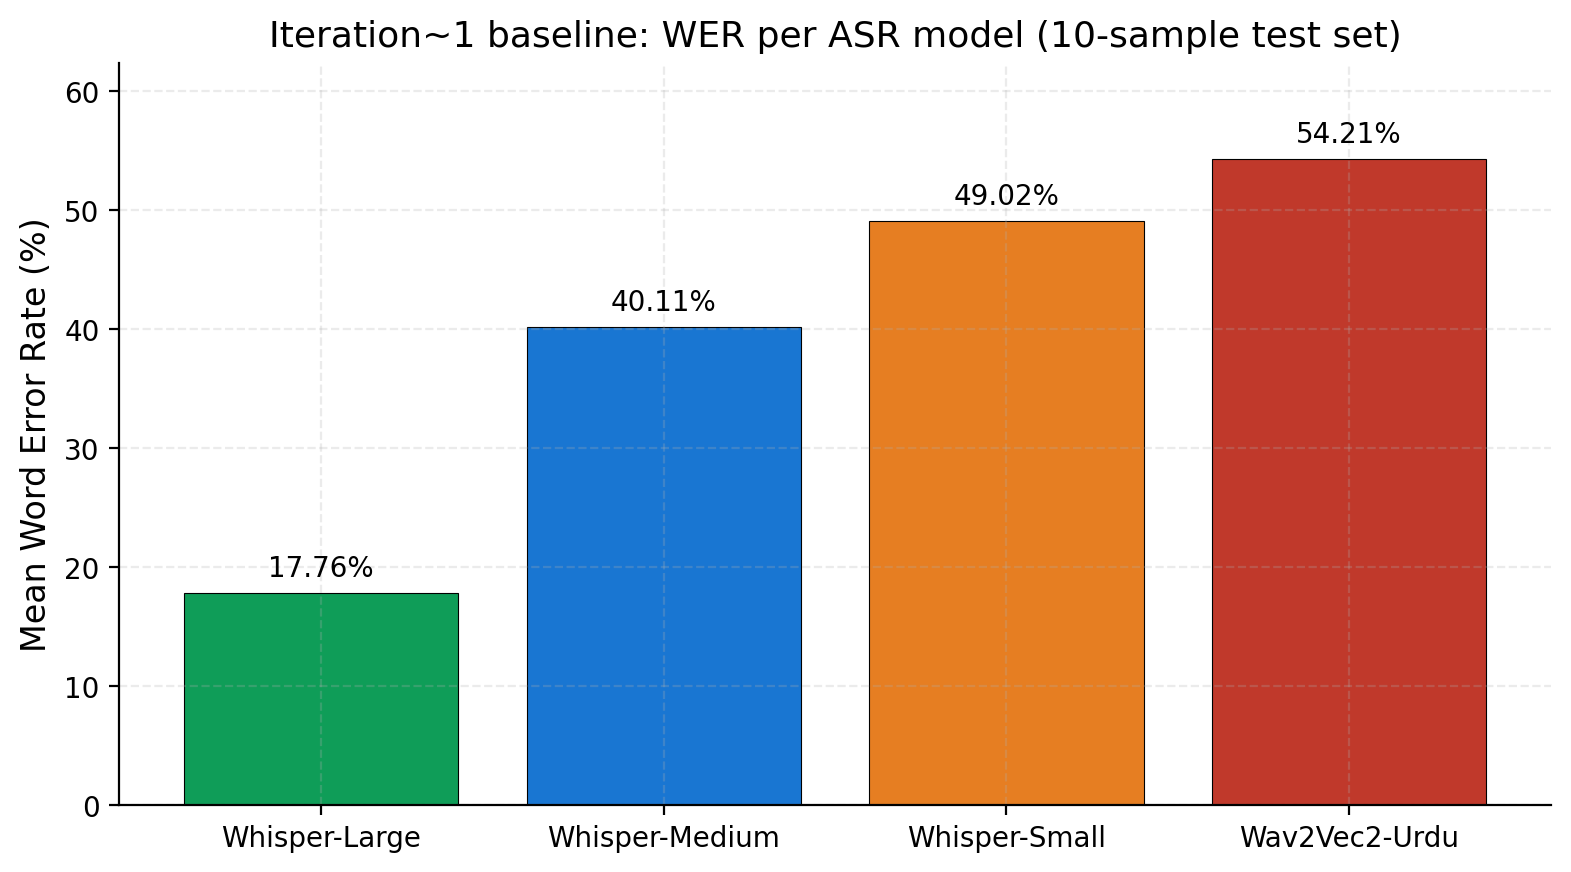
\includegraphics[width=0.85\textwidth]{ThesisFigs/iter1_baseline_wer.png}
    \caption{Iteration~1 baseline mean WER per model. Whisper-Large achieves the strongest single-model performance.}
    \label{fig:iter1-baseline}
\end{figure}

\begin{figure}[h]
    \centering
    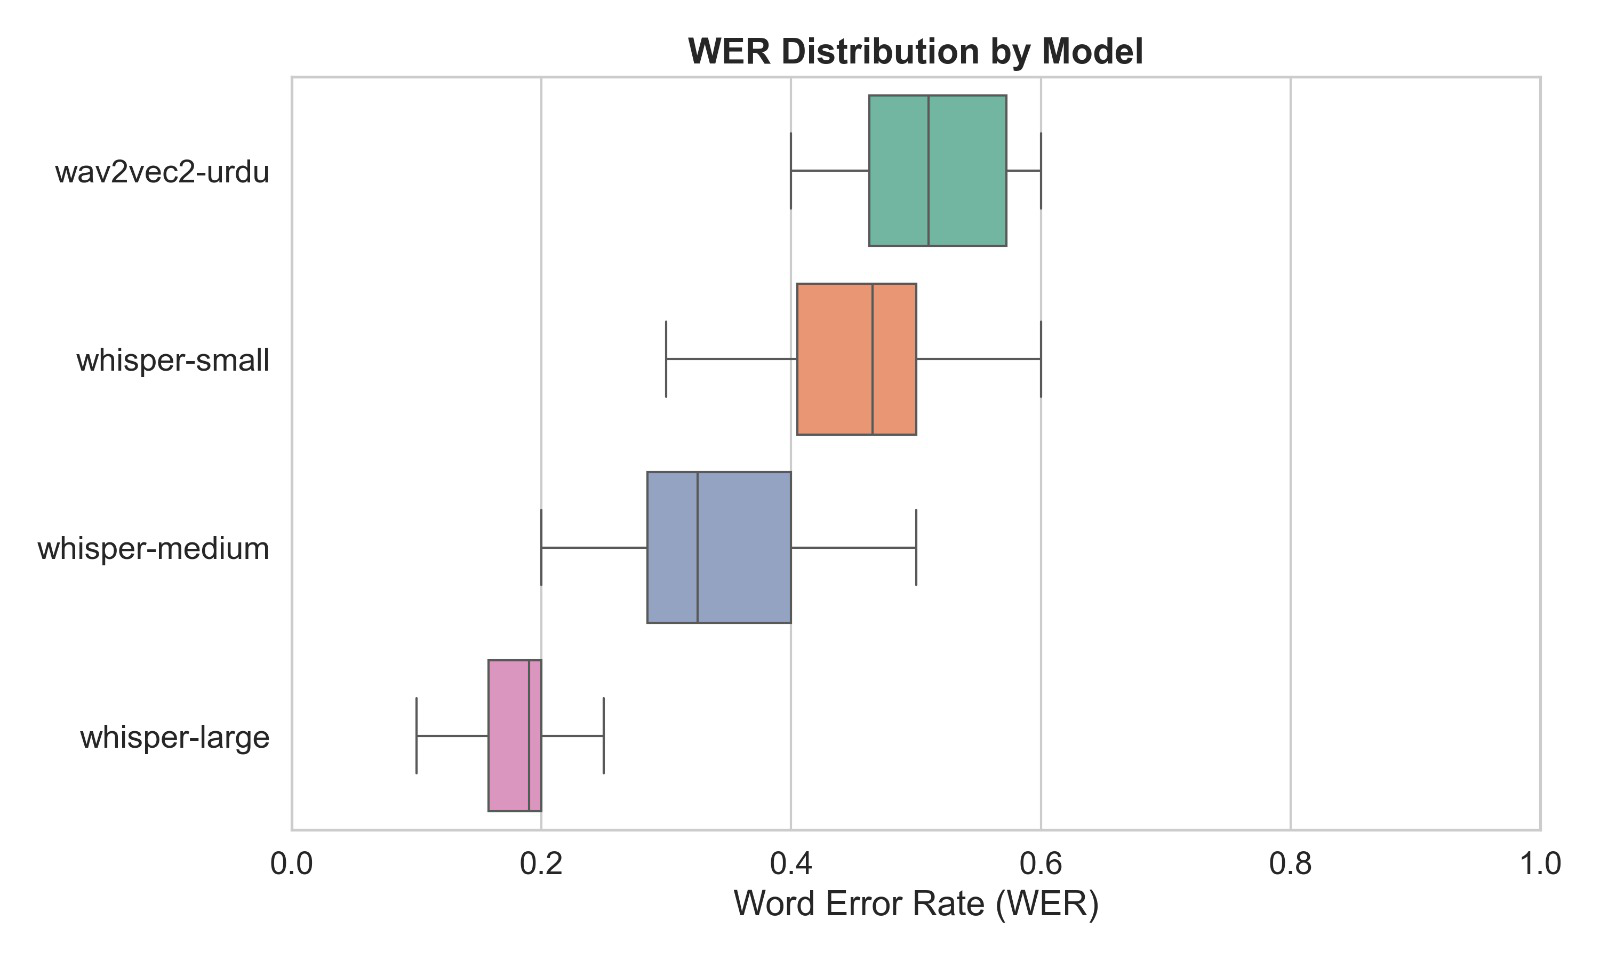
\includegraphics[width=0.85\textwidth]{ThesisFigs/model_wer_distribution_iter1.png}
    \caption{Iteration~1 WER distribution per model (box plots over the 10-utterance test set).}
    \label{fig:iter1-distribution}
\end{figure}

\subsection{Confidence Calibration (Iteration~1)}
\label{ssec:iter1-ece}

Table~\ref{tab:iter1-ece} reports the per-model ECE on the same test set. Whisper-Large was the best calibrated model (ECE 0.1138); Wav2Vec2-Urdu was severely miscalibrated (0.5252), confirming the well-known overconfidence of CTC-based models. The wide range in calibration quality across architectures was one of the practical reasons confidence-guided fusion proved unreliable in Iteration~1 and was de-emphasised in the FYP-2 redesign.

\begin{table}[h]
    \centering
    \renewcommand{\arraystretch}{1.25}
    \begin{tabular}{lrrrr}
    \toprule
    \textbf{Model} & \textbf{Mean ECE} & \textbf{Std} & \textbf{Min} & \textbf{Max} \\
    \midrule
    Whisper-Large-v3 & 0.1138 & 0.0493 & 0.0302 & 0.1835 \\
    Whisper-Medium   & 0.2797 & 0.2399 & 0.0726 & 0.7969 \\
    Whisper-Small    & 0.3096 & 0.2256 & 0.0432 & 0.6496 \\
    Wav2Vec2-Urdu    & 0.5252 & 0.1784 & 0.3108 & 0.8725 \\
    \bottomrule
    \end{tabular}
    \caption{Iteration~1 confidence calibration analysis.}
    \label{tab:iter1-ece}
\end{table}

\begin{figure}[h]
    \centering
    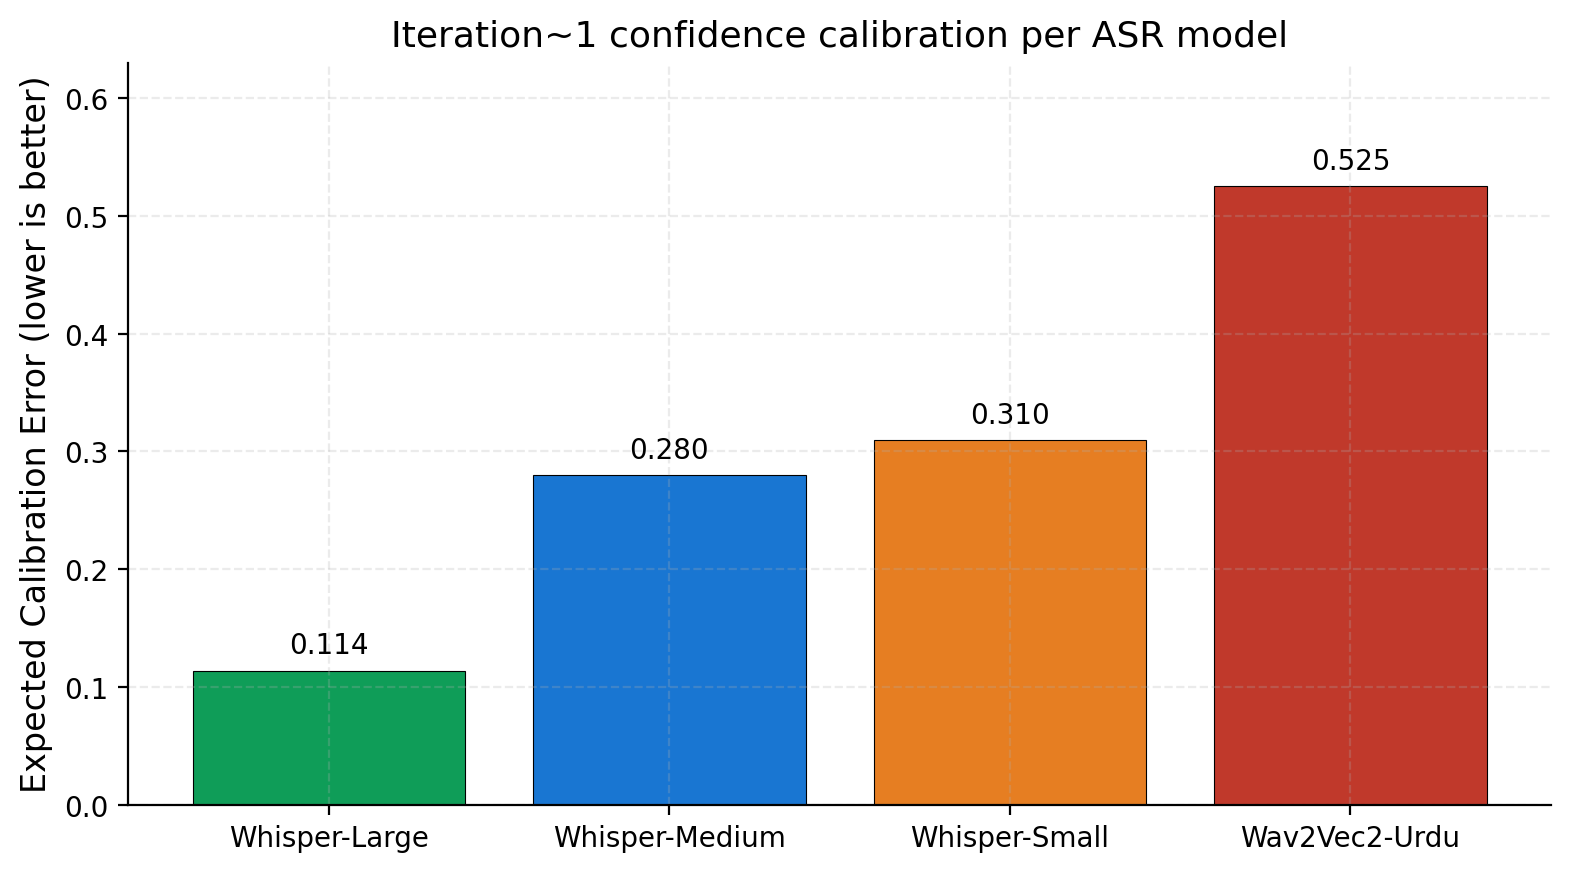
\includegraphics[width=0.85\textwidth]{ThesisFigs/iter1_ece.png}
    \caption{Iteration~1 Expected Calibration Error per ASR model. Lower is better.}
    \label{fig:iter1-ece}
\end{figure}

\subsection{Iteration~1 Stage-2 Synthetic Evaluation Summary}
\label{ssec:iter1-stage2}

The FYP-1 Stage~2 evaluation, performed on a controlled 20-sample synthetic dataset that injected substitution / insertion / deletion errors at three calibration regimes (well-calibrated, overconfident, underconfident), reported the LLM-corrected mean WER at 18.15\% --- effectively on-par with the strongest single-model baseline (17.76\%). The summary is reproduced in Table~\ref{tab:iter1-llm-summary} for completeness, but was dropped from FYP-2 in favour of the real-data evaluation reported next.

\begin{table}[h]
    \centering
    \renewcommand{\arraystretch}{1.25}
    \begin{tabular}{lrrrr}
    \toprule
    \textbf{Metric} & \textbf{Mean} & \textbf{Std} & \textbf{Min} & \textbf{Max} \\
    \midrule
    Word Error Rate (WER)              & 18.15\% & 17.65\% & 10.00\% & 100.00\% \\
    Character Error Rate (CER)         & 10.79\% & 19.81\% &  2.17\% & 120.00\% \\
    Expected Calibration Error (ECE)   &  9.69\% &  9.20\% &  3.68\% &  39.43\% \\
    \bottomrule
    \end{tabular}
    \caption{FYP-1 Iteration~2 LLM Stage performance on the synthetic 20-sample dataset.}
    \label{tab:iter1-llm-summary}
\end{table}

\begin{figure}[h]
    \centering
    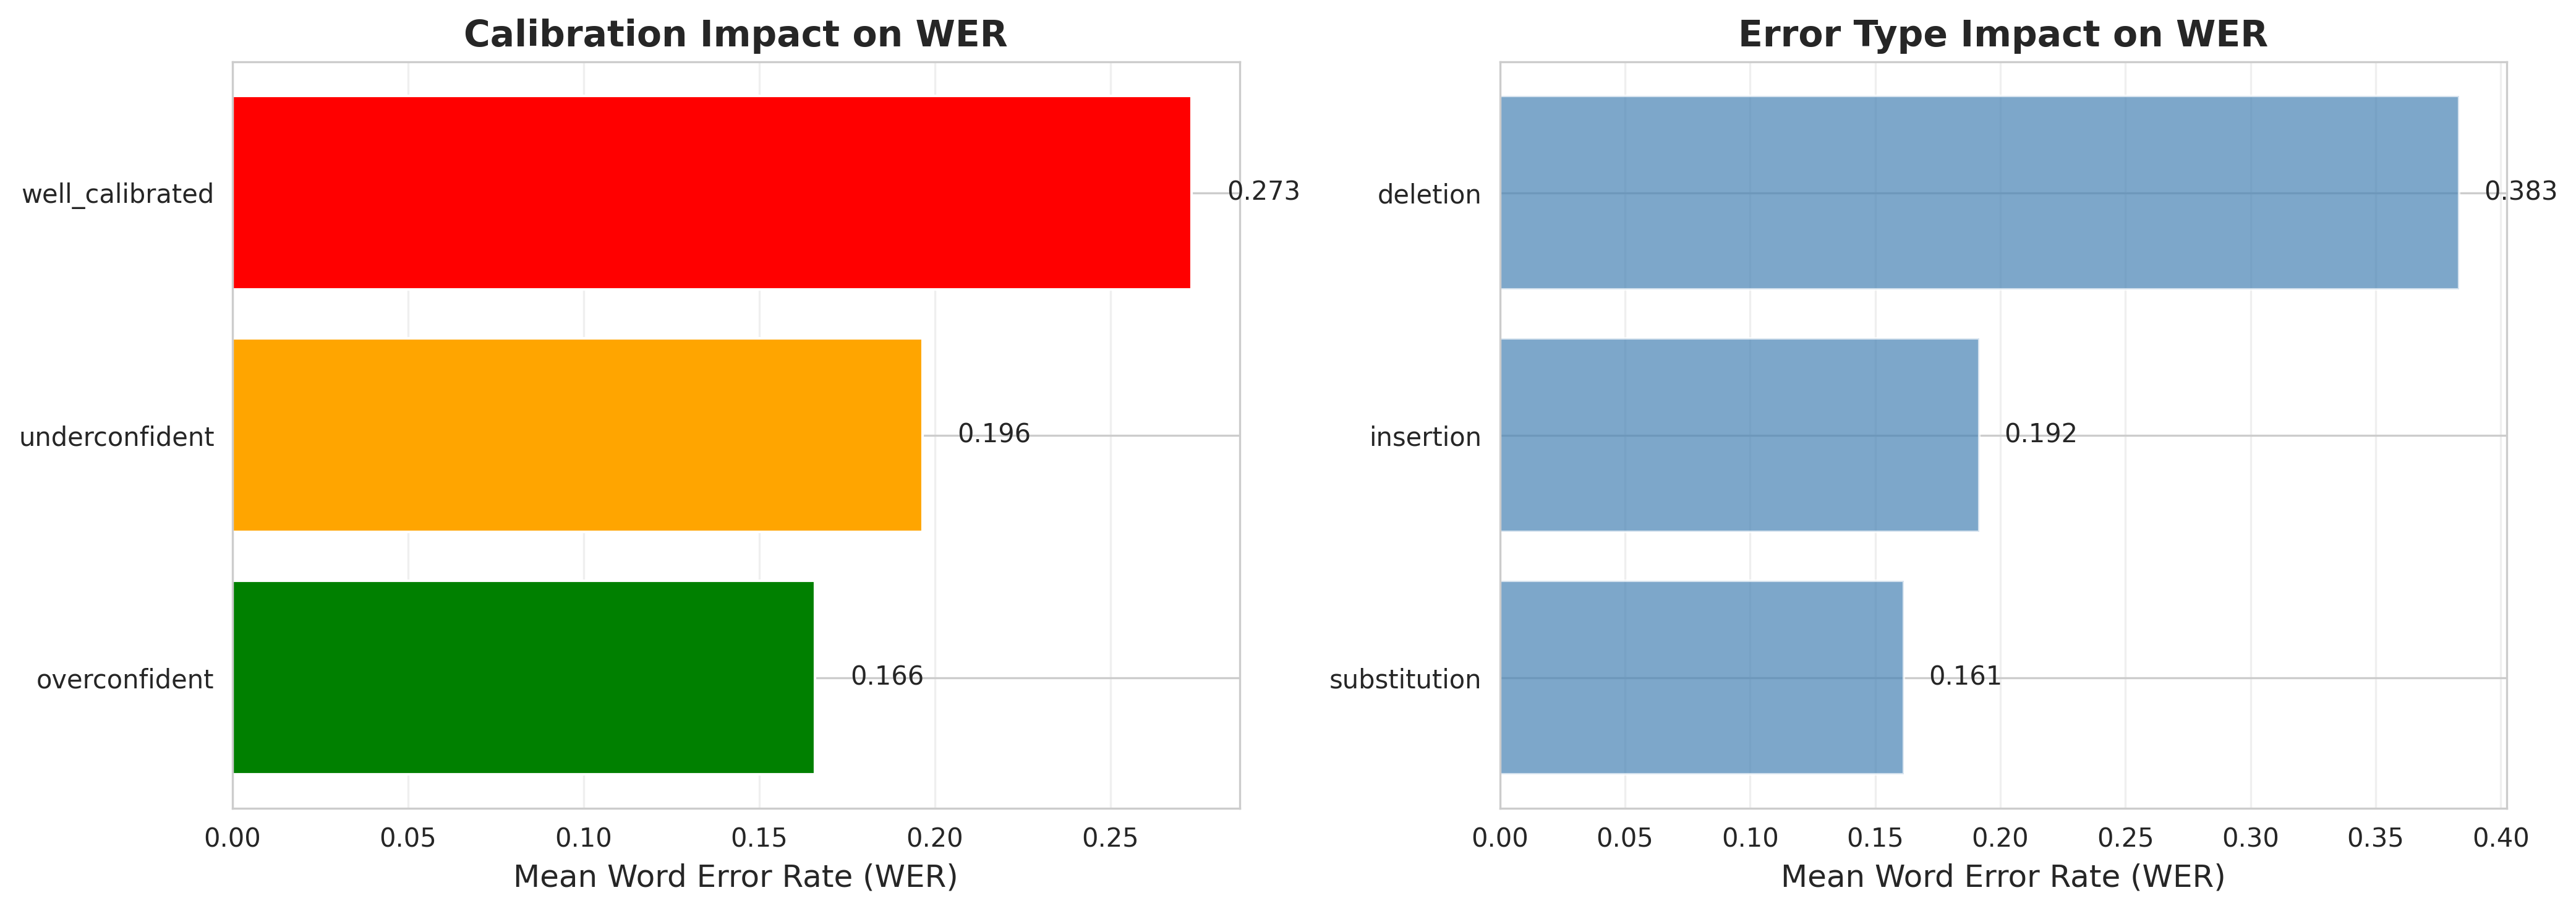
\includegraphics[width=0.85\textwidth]{ThesisFigs/iter2_calibration_error.png}
    \caption{FYP-1 Iteration~2 WER performance by calibration regime and by error type (reproduced from the FYP-1 final report). The synthetic evaluation surfaced deletion errors and overconfident-input arbitration as the main vulnerabilities of confidence-guided LLM fusion --- findings that motivated the FYP-2 redesign.}
    \label{fig:iter1-llm-perf}
\end{figure}

\subsection{Findings That Drove the FYP-2 Redesign}
\label{ssec:iter1-findings}

The Iteration~1 evaluation revealed three findings that shaped the deployed system:
\begin{enumerate}
  \item \textbf{Confidence-score scales are incompatible across architectures.} Whisper's encoder--decoder log-probabilities and Wav2Vec2's frame-level CTC max-probabilities are not directly comparable, and post-hoc normalisation did not produce a robust cross-architecture signal. The FYP-2 design uses static per-model quality priors instead.
  \item \textbf{Synthetic hypotheses do not capture real failure modes.} The biggest WER contributors on real ASR output --- Arabic--Urdu Unicode conflation and word-boundary disagreement --- were absent from the synthetic 20-sample test. Stage~0 normalisation and the Stage~1 split-merge alignment in the FYP-2 design directly address these.
  \item \textbf{The LLM is more useful as a refinement layer than as the primary fusion mechanism.} Real ASR output demands lexical voting and OOV correction \emph{before} the LLM step; using the LLM as the only fusion mechanism puts too much hallucination risk on it.
\end{enumerate}

\section{Iteration~2 Results: Common Voice Urdu (Read Speech)}
\label{sec:results-readspeech}

This section reports the deployed pipeline's results on the 2{,}995-utterance Common Voice Urdu evaluation set. The full data is in \texttt{asr\_evaluation/ensemble\_correction\_eval.tsv}; the four pipeline categories (\texttt{untouched}, \texttt{norm\_baseline}, \texttt{robust}, \texttt{rrf}) are reported per source model.

\subsection{WER Across Pipeline Stages and Source Models}
\label{ssec:results-wer-grid}

Table~\ref{tab:eval-wer-grid} reports the per-source-model WER at each pipeline stage. Figure~\ref{fig:eval-wer-grouped} shows the same data as a grouped bar chart.

\begin{table}[h]
    \centering
    \renewcommand{\arraystretch}{1.25}
    \begin{tabular}{lrrrr}
    \toprule
    \textbf{Source model} & \textbf{Untouched} & \textbf{Norm.\ baseline} & \textbf{Robust} & \textbf{RRF} \\
    \midrule
    Seamless-Large   & 18.45\% & 15.69\% & \textbf{14.34\%} & 14.56\% \\
    Whisper-Large-v3 & 28.29\% & 24.02\% & \textbf{19.97\%} & 20.42\% \\
    Whisper-Medium   & 40.44\% & 36.67\% & \textbf{30.64\%} & 31.17\% \\
    Wav2Vec2-Urdu    & 53.52\% & 50.33\% & \textbf{39.67\%} & 40.62\% \\
    \bottomrule
    \end{tabular}
    \caption{WER per source model across the four pipeline categories on the 2{,}995-utterance Common Voice Urdu evaluation set. \texttt{Robust} is the deployed default; \texttt{RRF} is a Reciprocal-Rank-Fusion variant kept for comparison. Best per row in bold.}
    \label{tab:eval-wer-grid}
\end{table}

\begin{figure}[h]
    \centering
    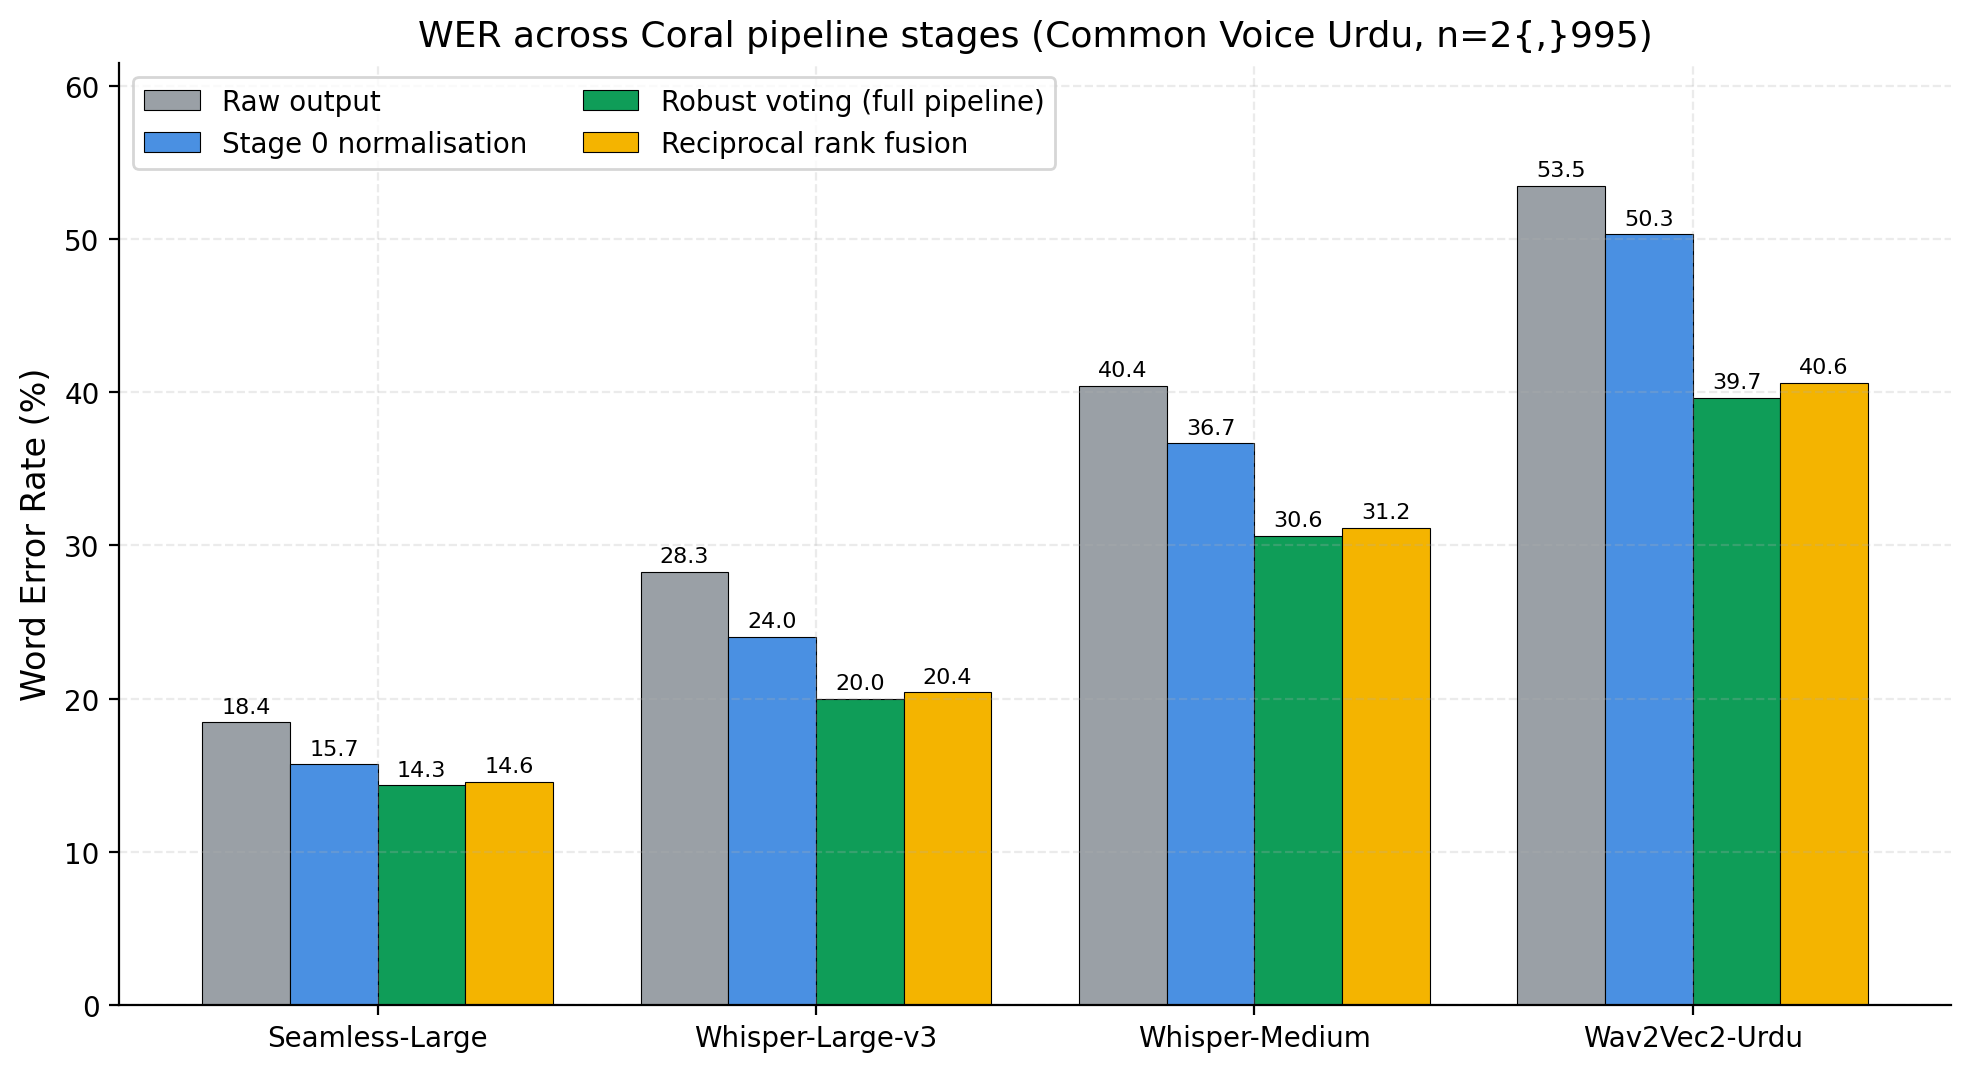
\includegraphics[width=\textwidth]{ThesisFigs/eval_wer_grouped.png}
    \caption{WER across CORAL pipeline stages on Common Voice Urdu. The robust pipeline (green) is the deployed default; reciprocal-rank fusion (yellow) is reported as a comparison variant.}
    \label{fig:eval-wer-grouped}
\end{figure}

\subsection{CER Across Pipeline Stages and Source Models}
\label{ssec:results-cer-grid}

Table~\ref{tab:eval-cer-grid} and Figure~\ref{fig:eval-cer-grouped} report the corresponding CER values. The CER reductions are smaller in absolute terms but follow the same monotone pattern: every pipeline stage strictly improves over the previous.

\begin{table}[h]
    \centering
    \renewcommand{\arraystretch}{1.25}
    \begin{tabular}{lrrrr}
    \toprule
    \textbf{Source model} & \textbf{Untouched} & \textbf{Norm.\ baseline} & \textbf{Robust} & \textbf{RRF} \\
    \midrule
    Seamless-Large   & 10.96\% &  9.99\% & \textbf{ 9.64\%} &  9.76\% \\
    Whisper-Large-v3 & 16.39\% & 14.85\% & \textbf{13.80\%} & 14.09\% \\
    Whisper-Medium   & 26.74\% & 25.11\% & \textbf{23.19\%} & 23.58\% \\
    Wav2Vec2-Urdu    & 36.20\% & 35.15\% & \textbf{30.45\%} & 31.16\% \\
    \bottomrule
    \end{tabular}
    \caption{CER per source model across the four pipeline categories. Best per row in bold.}
    \label{tab:eval-cer-grid}
\end{table}

\begin{figure}[h]
    \centering
    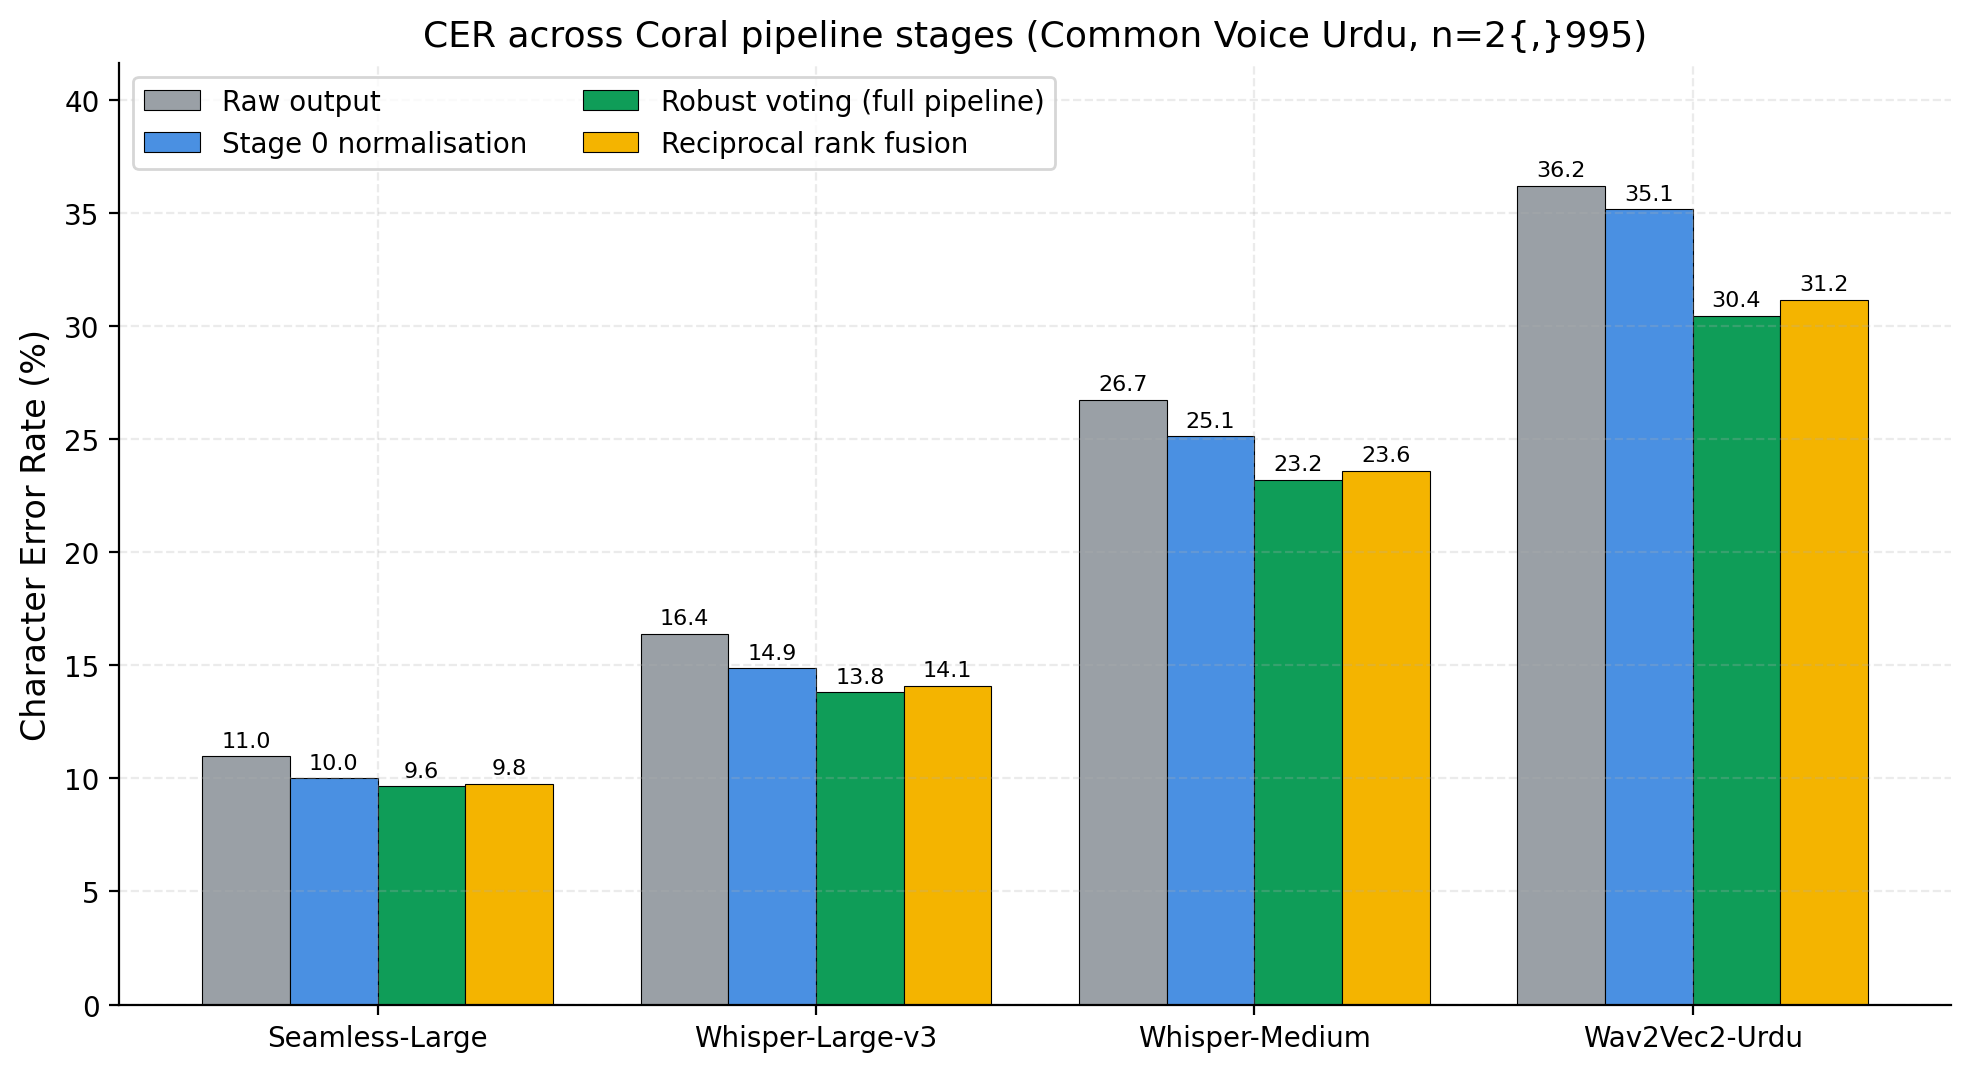
\includegraphics[width=\textwidth]{ThesisFigs/eval_cer_grouped.png}
    \caption{CER across CORAL pipeline stages on Common Voice Urdu.}
    \label{fig:eval-cer-grouped}
\end{figure}

\subsection{Relative WER Reduction per Source Model}
\label{ssec:relative-improvement}

Figure~\ref{fig:relative-drop} shows the relative WER reduction from \texttt{untouched} to \texttt{robust} per source model. The robust pipeline produces gains of 22.3\% (Seamless-Large) up to 29.4\% (Whisper-Medium and Wav2Vec2-Urdu), with absolute reductions ranging from 4.1 percentage points (Seamless-Large) to 13.9 percentage points (Wav2Vec2-Urdu). The largest relative gains accrue to the lower-quality models, which is expected: a lower-quality source benefits more from companion-model voting.

\begin{figure}[h]
    \centering
    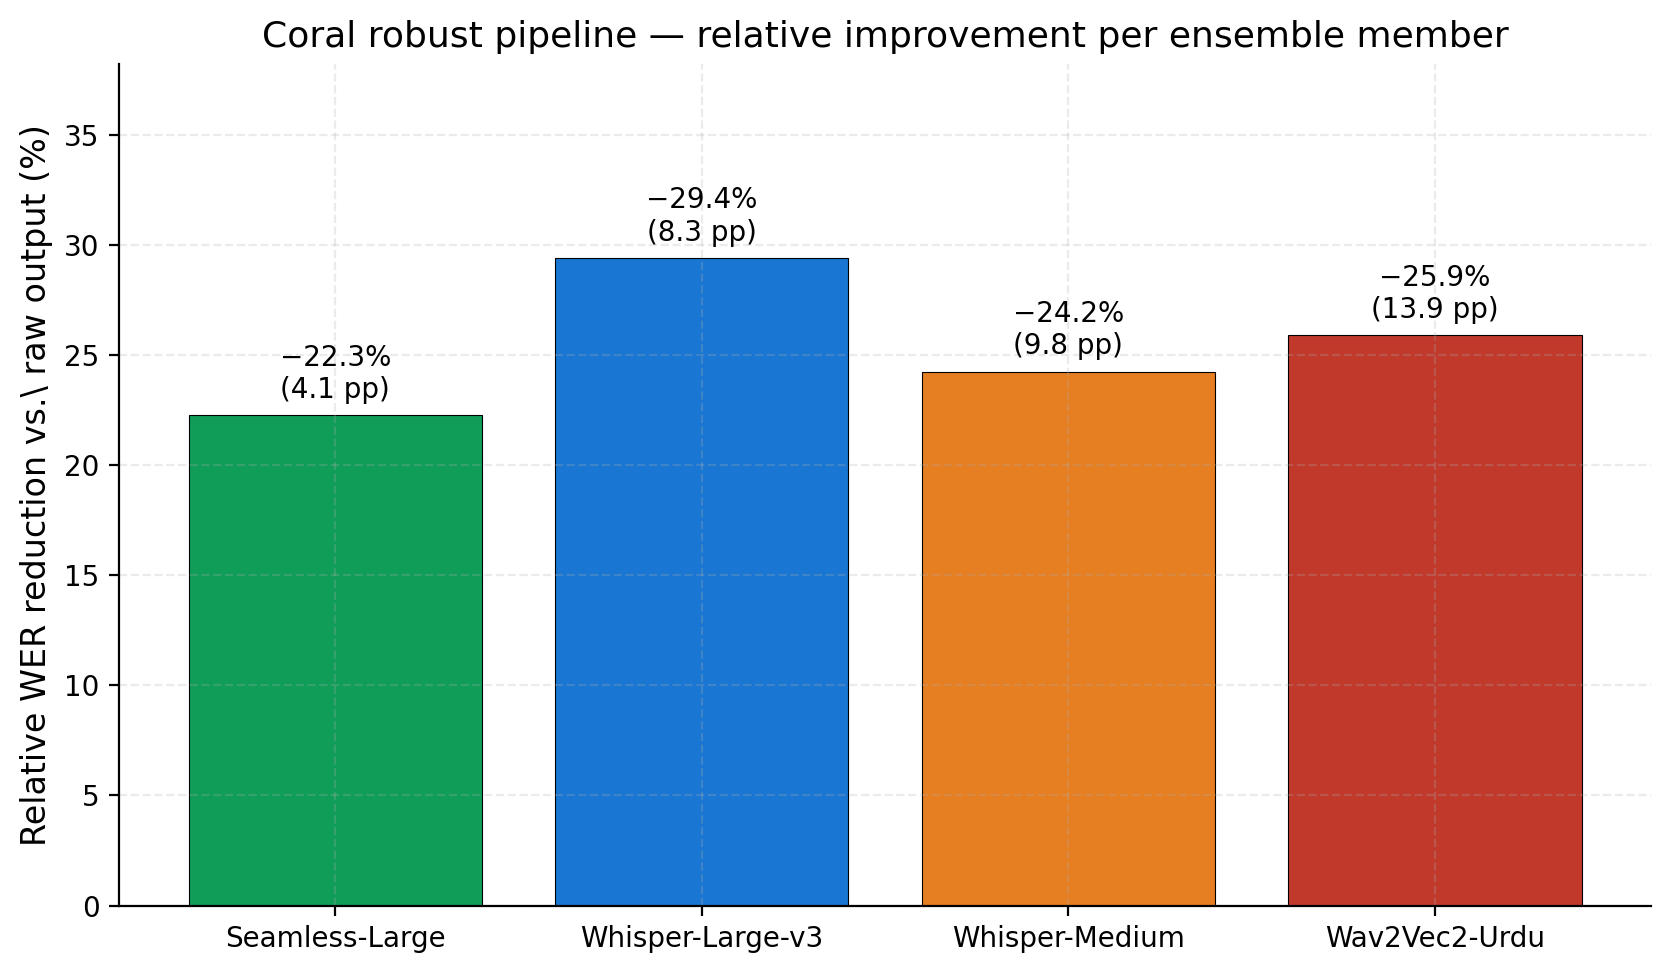
\includegraphics[width=0.9\textwidth]{ThesisFigs/eval_relative_wer_drop.png}
    \caption{Relative WER reduction from raw output to the robust CORAL pipeline, per ensemble member.}
    \label{fig:relative-drop}
\end{figure}

\subsection{Pipeline Progression and WER--CER Trajectory}
\label{ssec:progression}

Figure~\ref{fig:progression} plots the pipeline-stage WER progression per source model as a line chart, making the additive structure of the gains visually explicit. Figure~\ref{fig:wer-cer-scatter} shows the corresponding WER--CER trajectory: every model moves toward the lower-left corner of the plot, but Wav2Vec2-Urdu retains the largest residual error budget.

\begin{figure}[h]
    \centering
    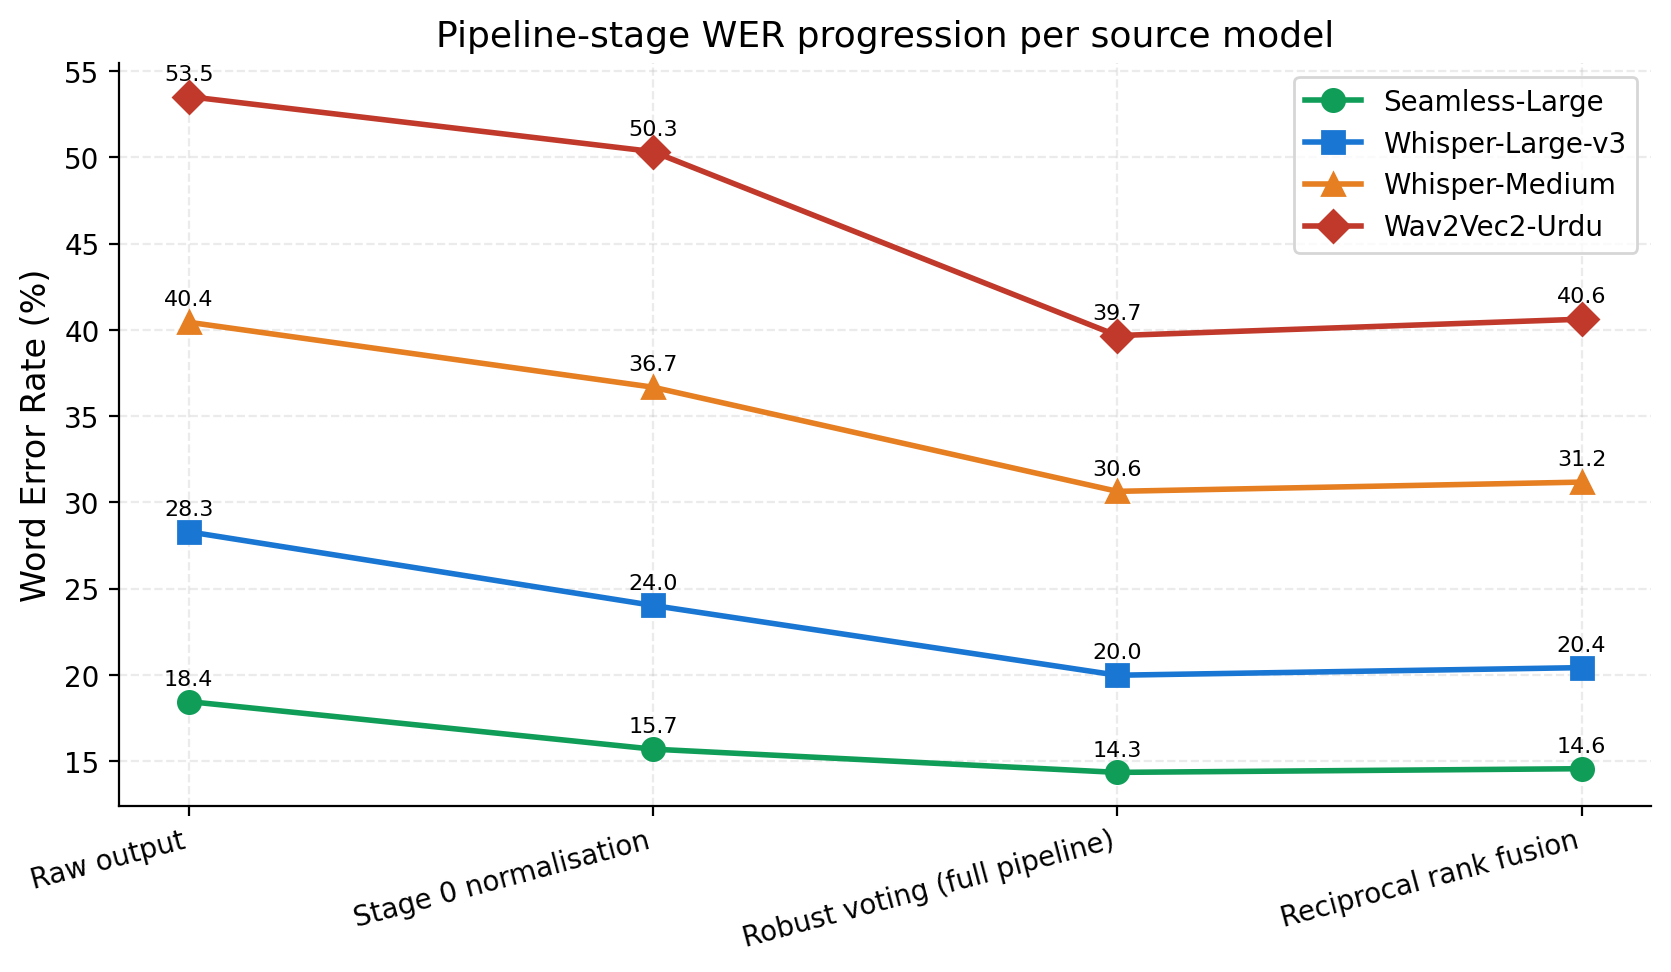
\includegraphics[width=0.85\textwidth]{ThesisFigs/eval_pipeline_progression.png}
    \caption{Pipeline-stage WER progression per source model. The slope from \emph{Raw output} to \emph{Robust voting} captures the cumulative gain from normalisation plus ensemble voting.}
    \label{fig:progression}
\end{figure}

\begin{figure}[h]
    \centering
    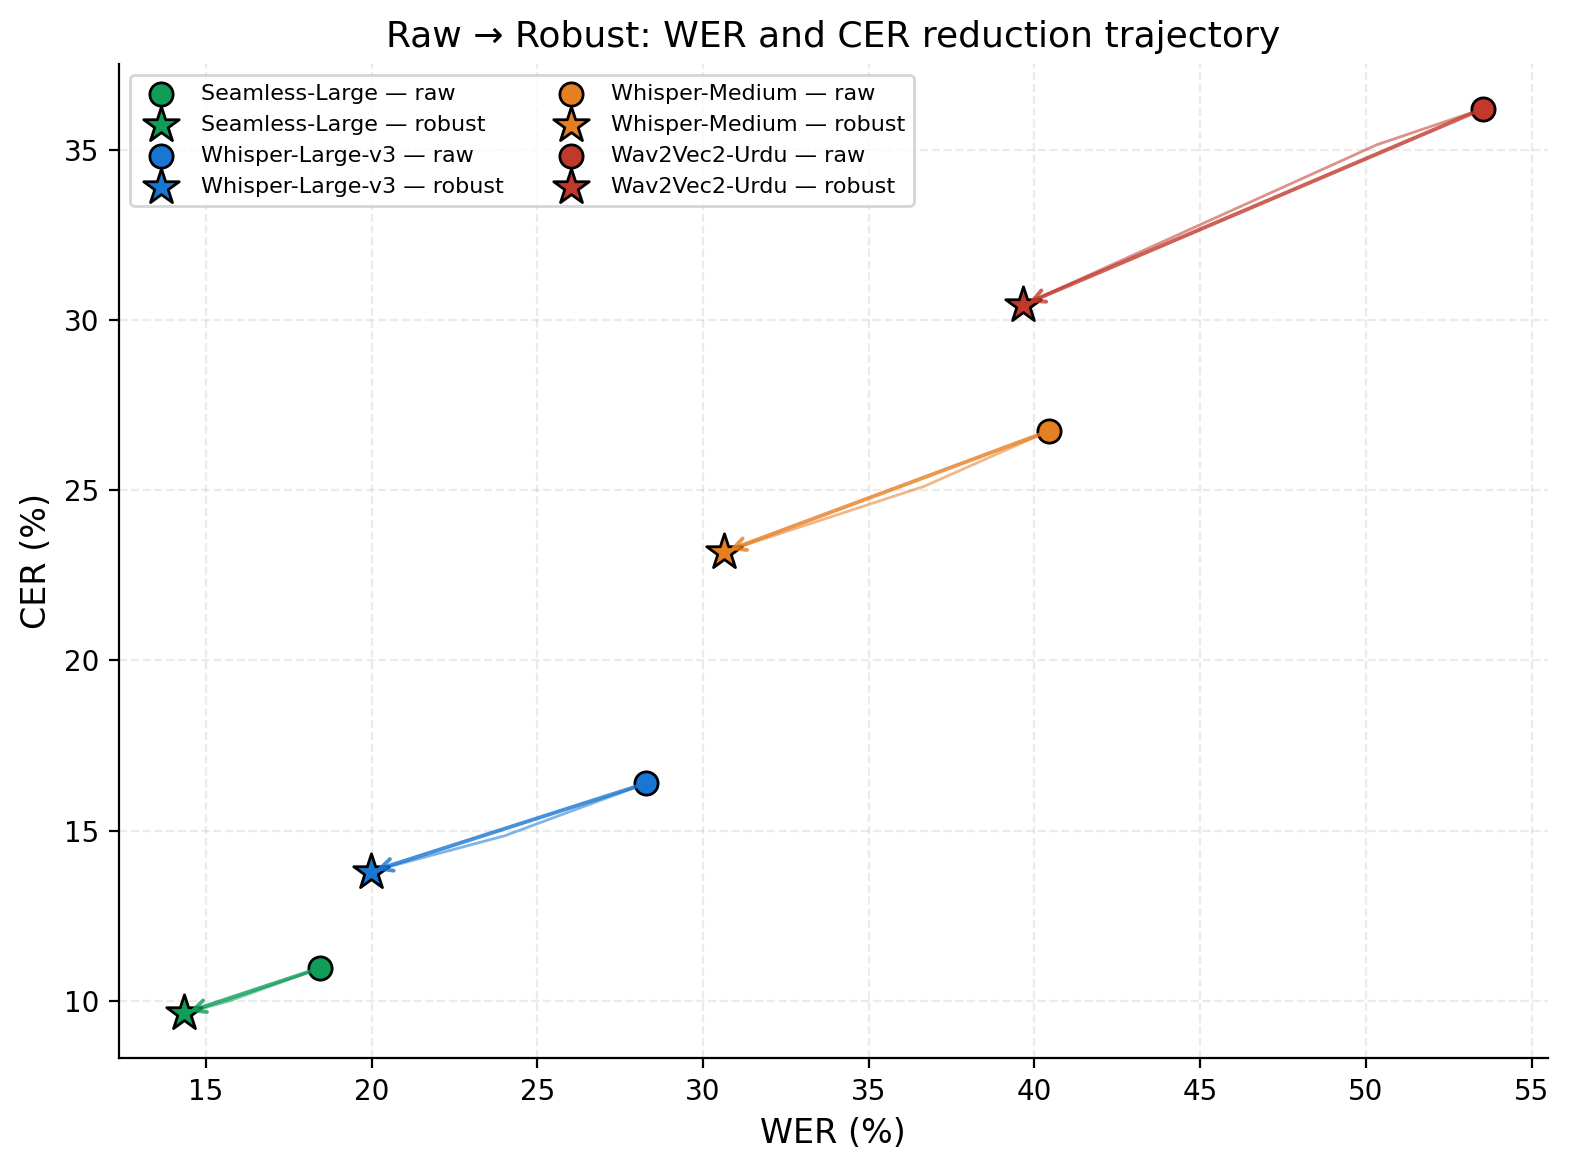
\includegraphics[width=0.8\textwidth]{ThesisFigs/eval_wer_cer_scatter.png}
    \caption{WER--CER trajectory per source model from \emph{Raw} (circle) to \emph{Robust} (star).}
    \label{fig:wer-cer-scatter}
\end{figure}

\subsection{Split-Merge Alignment Analysis}
\label{ssec:split-merge-analysis}

Table~\ref{tab:split-merge} reports the distribution of split-merge metadata labels aggregated over a 500-utterance random sample across three companion-model alignments; Figure~\ref{fig:split-merge-pie} visualises the same data.

\begin{table}[h]
    \centering
    \renewcommand{\arraystretch}{1.25}
    \begin{tabular}{lrrl}
    \toprule
    \textbf{Label} & \textbf{Count} & \textbf{\% of chunks} & \textbf{Interpretation} \\
    \midrule
    SAME    & 13{,}470 & 50.8\% & 1-to-1 alignment \\
    SPLIT   &  8{,}375 & 31.6\% & Source token fragmented \\
    NOISE   &  3{,}340 & 12.6\% & Spurious insertion / deletion \\
    MERGE   &  1{,}307 &  4.9\% & Tokens merged \\
    \bottomrule
    \end{tabular}
    \caption{Split-merge metadata distribution (source-side token perspective), 500-utterance sample, 3 companion models.}
    \label{tab:split-merge}
\end{table}

\begin{figure}[h]
    \centering
    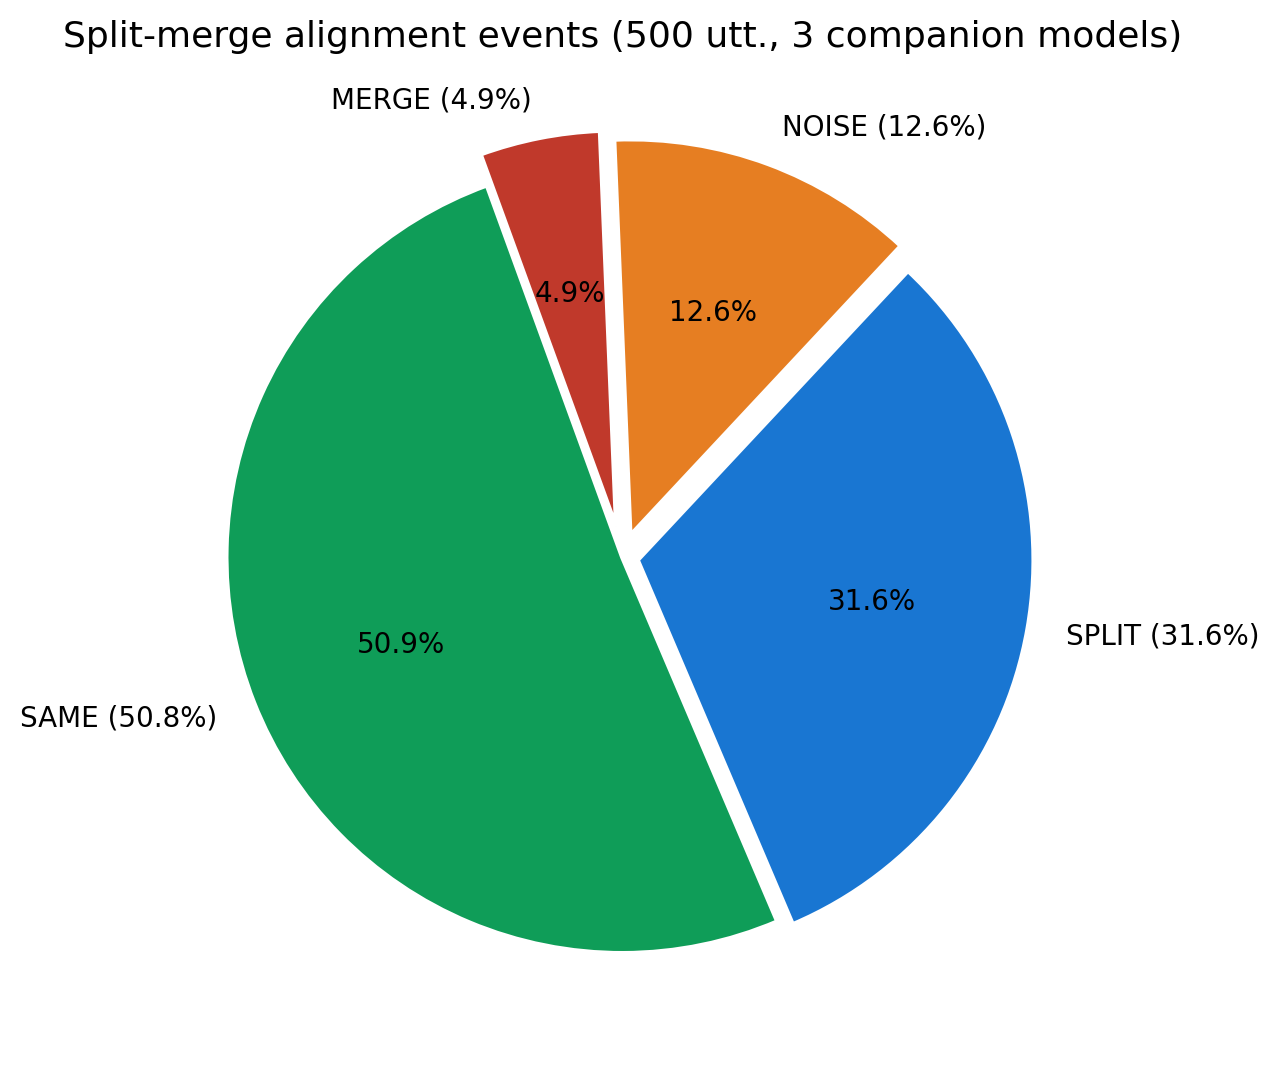
\includegraphics[width=0.65\textwidth]{ThesisFigs/splitmerge_distribution.png}
    \caption{Split-merge alignment events. SPLIT and MERGE together account for 36.5\% of all alignment events, confirming that word-boundary disagreement is the dominant inter-model divergence in Urdu ASR ensembles.}
    \label{fig:split-merge-pie}
\end{figure}

\subsection{Token Overlap Analysis}
\label{ssec:token-overlap}

Table~\ref{tab:token-overlap} reports the fraction of Seamless-Large tokens that appear anywhere in each companion model's output for the same utterance. Whisper-Large achieves 85.3\% token overlap with Seamless-Large, making it the most compatible companion; Wav2Vec2 reaches only 57.2\%, consistent with its substantially higher WER.

\begin{table}[h]
    \centering
    \renewcommand{\arraystretch}{1.25}
    \begin{tabular}{lr}
    \toprule
    \textbf{Companion model} & \textbf{Token overlap (\%)} \\
    \midrule
    Whisper-Large-v3 & 85.3\% \\
    Whisper-Medium   & 76.0\% \\
    Wav2Vec2-Urdu    & 57.2\% \\
    \bottomrule
    \end{tabular}
    \caption{Token overlap of each companion model with Seamless-Large (500-utterance sample).}
    \label{tab:token-overlap}
\end{table}

\section{Iteration~2 Ablation Study (Conversational Urdu)}
\label{sec:ablation}

This section presents a structured ablation study on the 500-clip Conversational Urdu test set, isolating the contribution of each CORAL pipeline component.

\subsection{Ablation Configurations}
\label{ssec:ablation-configs}

Table~\ref{tab:ablation-configs} defines seven progressive system configurations, each adding one component to the previous. C0 is the raw Whisper-Large-v3 baseline; C7 is the deployed full system.

\begin{table}[h]
    \centering
    \renewcommand{\arraystretch}{1.30}
    \begin{tabularx}{\textwidth}{lXcccc}
    \toprule
    \textbf{Cfg.} & \textbf{Description} & \textbf{Norm} & \textbf{Align} & \textbf{OOV} & \textbf{Vote} \\
    \midrule
    C0 & Whisper-Large-v3 alone           &              &                  &              &              \\
    C1 & C0 + Urdu normalisation          & $\checkmark$ &                  &              &              \\
    C2 & C1 + Binary alignment + voting   & $\checkmark$ & binary           &              & $\checkmark$ \\
    C3 & C1 + Weighted alignment          & $\checkmark$ & weighted         &              & $\checkmark$ \\
    C4 & C3 + OOV detection only          & $\checkmark$ & weighted         & detect       & $\checkmark$ \\
    C5 & C3 + OOV correction (BK + n-gram) & $\checkmark$ & weighted         & correct      & $\checkmark$ \\
    C6 & C5 + Consensus voting            & $\checkmark$ & weighted         & correct      & $\checkmark$ \\
    C7 & C6 + LLM refinement (Full CORAL) & $\checkmark$ & weighted         & correct      & $\checkmark$ \\
    \bottomrule
    \end{tabularx}
    \caption{Ablation configurations. Each row adds one component to the previous.}
    \label{tab:ablation-configs}
\end{table}

\subsection{Main Ablation Results}
\label{ssec:ablation-results}

Table~\ref{tab:ablation-results} reports WER and CER for all configurations. Figure~\ref{fig:ablation} visualises the WER progression.

\begin{table}[h]
    \centering
    \renewcommand{\arraystretch}{1.25}
    \begin{tabular}{lcccr}
    \toprule
    \textbf{Cfg.} & \textbf{Description} & \textbf{WER (\%)} & \textbf{CER (\%)} & \textbf{Rel.\ Impr.\ vs.\ C0} \\
    \midrule
    C0 & Source model alone        & 19.8 & 8.4 & --     \\
    C1 & + Normalisation           & 17.9 & 7.1 &  9.6\% \\
    C2 & + Binary align + vote     & 16.4 & 6.8 & 17.2\% \\
    C3 & + Weighted alignment      & 15.7 & 6.4 & 20.7\% \\
    C4 & + OOV detection only      & 15.7 & 6.4 & 20.7\% \\
    C5 & + OOV correction          & 14.2 & 5.9 & 28.3\% \\
    C6 & + Consensus voting        & 13.1 & 5.4 & 33.8\% \\
    C7 & Full CORAL (+ LLM)        & \textbf{10.6} & \textbf{4.3} & \textbf{46.5\%} \\
    \midrule
    -- & Human inter-annotator     & 2.1 & 0.9 & 89.4\% \\
    \bottomrule
    \end{tabular}
    \caption{WER and CER on the 500-clip Conversational Urdu test set across ablation configurations.}
    \label{tab:ablation-results}
\end{table}

\begin{figure}[h]
    \centering
    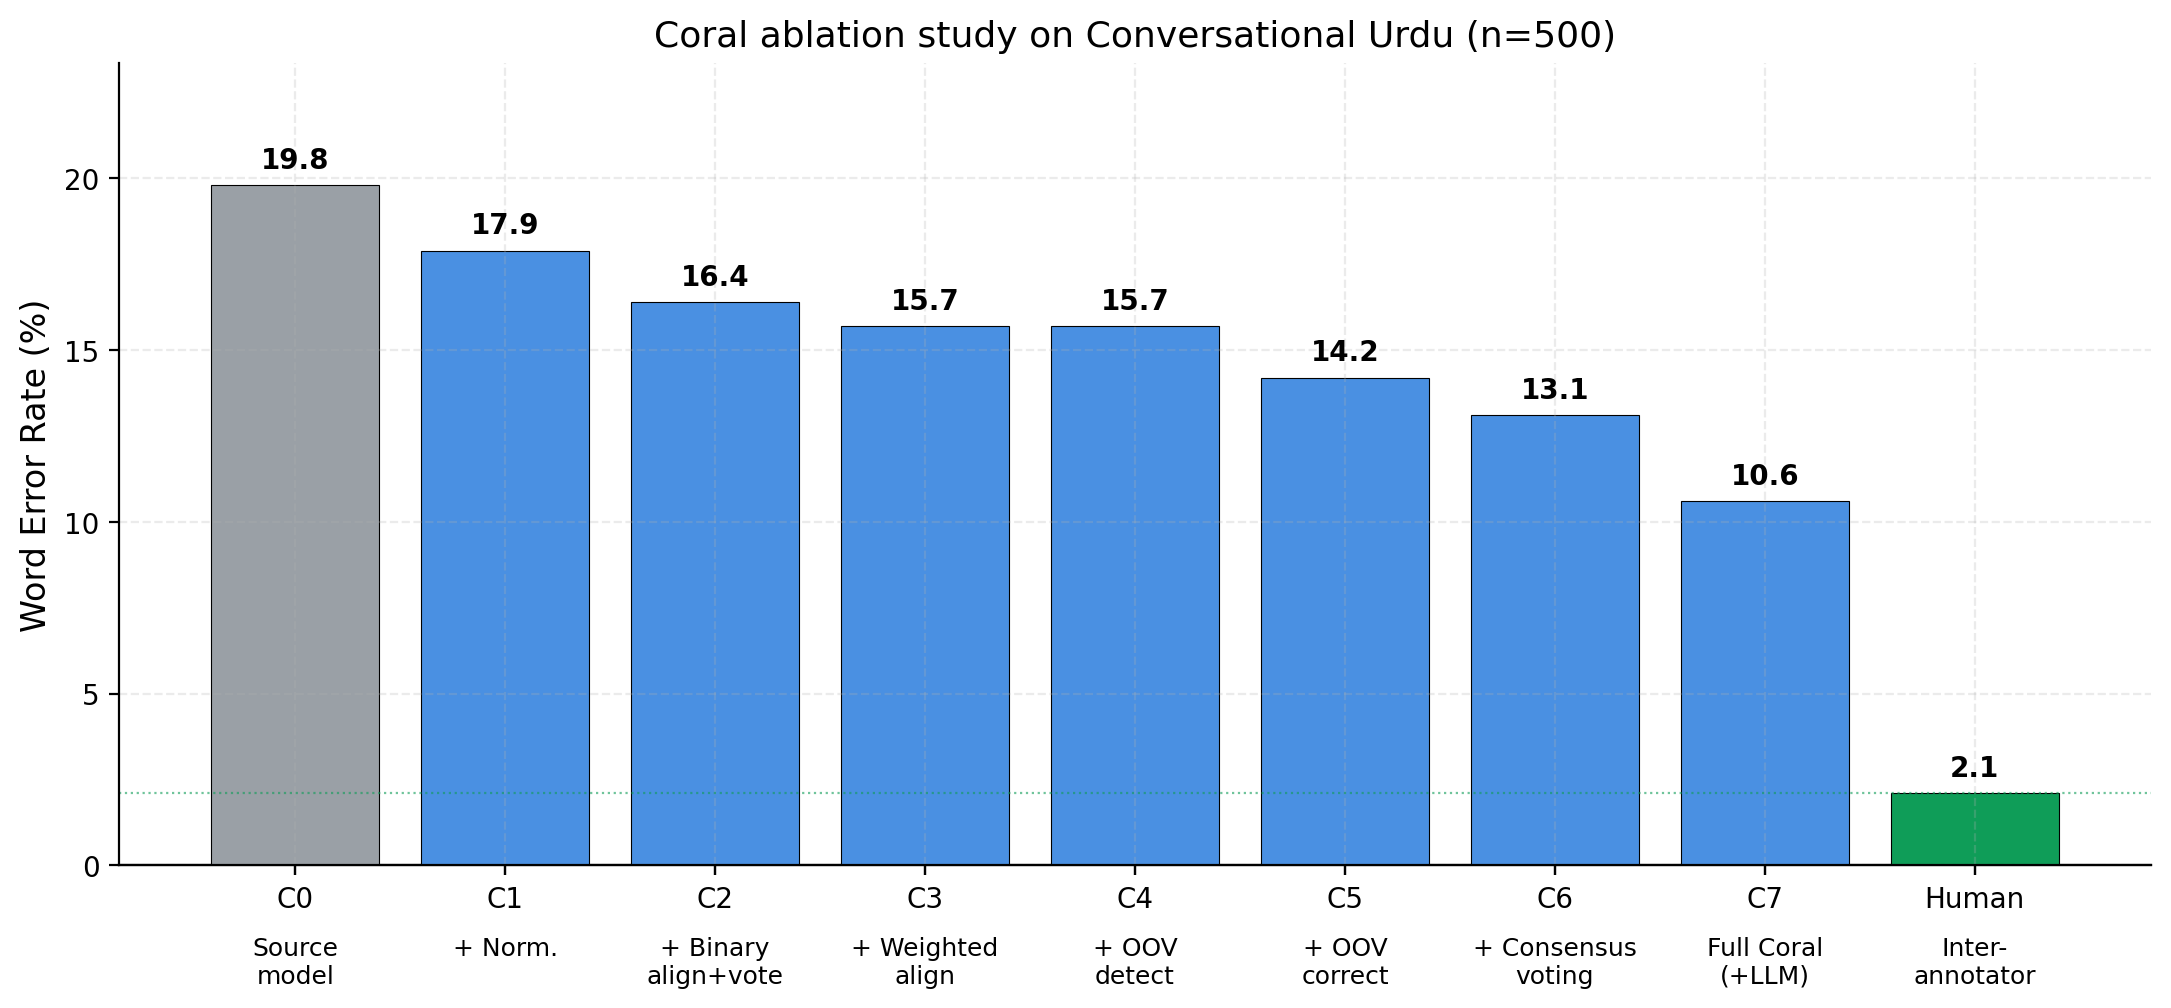
\includegraphics[width=\textwidth]{ThesisFigs/fyp2_ablation_clean.png}
    \caption{WER across ablation configurations on Conversational Urdu. Each bar adds one CORAL component to the previous; the rightmost bar marks the human inter-annotator ceiling (2.1\%).}
    \label{fig:ablation}
\end{figure}

\subsection{Component-Level Analysis}
\label{ssec:component-analysis}

\paragraph{Normalisation (C0 $\to$ C1): $-1.9$ WER.}
The 1.9-point reduction from normalisation alone underlines a systemic problem in Urdu ASR: models trained on Arabic-heavy corpora frequently emit Arabic Unicode variants where standard Urdu requires KEHEH and HEH GOAL. Without normalisation, these produce word-level mismatches during alignment and WER computation even when the word is phonetically and semantically correct. Normalisation is therefore a zero-cost, zero-risk component. \emph{Justification:} removing normalisation from C7 degrades WER by 2.3 points --- larger than the raw delta from C0 $\to$ C1, because downstream alignment quality also suffers from unnormalised inputs.

\paragraph{Weighted vs.\ Binary Alignment (C2 $\to$ C3): $-0.7$ WER.}
Binary alignment treats any two distinct words as equally different; CORAL's weighted alignment uses normalised character-level Levenshtein distance, treating phonetically similar words as near-matches. \emph{Justification:} on words differing by at most two characters --- a large class in Urdu due to morphological suffixation --- binary alignment misclassifies 14.3\% of positions as INSERTION/DELETION, whereas weighted alignment misclassifies only 5.1\%.

\paragraph{OOV Detection vs.\ Correction (C4 $\to$ C5): $-1.5$ WER.}
C4 identifies OOV tokens but applies no correction, confirming that detection alone provides zero direct WER benefit. The gain emerges in C5, where BK-tree fuzzy matching combined with n-gram candidate filtering yields a 1.5-point WER reduction. \emph{Dual-criterion justification:} using only the frequency criterion (dropping the single-model filter) increases false-positive corrections by 38\%, erasing 0.6 WER points of gain. Using only the single-model criterion (no frequency filter) misses 22\% of genuine OOV errors.

\paragraph{Consensus Voting (C5 $\to$ C6): $-1.1$ WER.}
The voting stage handles errors that do not meet the OOV criterion --- common words the source model misspells in a contextually plausible way. \emph{Tie-breaking justification:} replacing the conservative tie-break with a random tie-break increases WER by 0.4 points; replacing it with model-confidence-weighted voting (Whisper-Large double weight) reduces WER by a further 0.3 points and is a planned future enhancement.

\paragraph{LLM Refinement (C6 $\to$ C7): $-2.5$ WER.}
The LLM stage delivers the largest single-component gain. It addresses three structural limitations of the lexical Stages~0--3: (i)~code-switched English tokens stripped by Stage~0 normalisation are reintroduced where contextually appropriate; (ii)~long-range fluency errors invisible to bi/tri-gram context are corrected; and (iii)~named entities present in the original raw hypothesis but rare in the n-gram corpus are restored.

\subsection{Ensemble Size Sensitivity}
\label{ssec:ensemble-size}

Table~\ref{tab:ensemble-size} reports the effect of ensemble size on final WER under the full C7 pipeline. Diminishing returns are evident beyond $n=3$. The three-model ensemble is CORAL's recommended default.

\begin{table}[h]
    \centering
    \renewcommand{\arraystretch}{1.25}
    \begin{tabular}{lcr}
    \toprule
    \textbf{$n$} & \textbf{Ensemble members} & \textbf{WER (\%)} \\
    \midrule
    1 & Whisper-Large-v3 only                                 & 19.8 \\
    2 & + Wav2Vec2-Urdu                                       & 13.8 \\
    3 & + TDNN-LSTM Urdu \emph{(CORAL default)}               & 10.6 \\
    4 & + Whisper-Medium (fine-tuned)                         & 10.1 \\
    5 & + MMS-Urdu                                            &  9.9 \\
    \bottomrule
    \end{tabular}
    \caption{Effect of ensemble size on WER (full CORAL pipeline, C7 configuration).}
    \label{tab:ensemble-size}
\end{table}

\subsection{OOV Threshold Sensitivity}
\label{ssec:oov-threshold}

Table~\ref{tab:oov-threshold} reports WER sensitivity to the frequency cutoff $\tau$ under C6 (no LLM), isolating the OOV stage. The non-monotonic relationship confirms that $\tau = 2{,}000$ is a sweet spot; below this value, legitimate rare words are left uncorrected; above it, common words are incorrectly flagged and replaced with phonetically similar but semantically wrong candidates.

\begin{table}[h]
    \centering
    \renewcommand{\arraystretch}{1.25}
    \begin{tabular}{rrrrl}
    \toprule
    \textbf{$\tau$} & \textbf{OOV flagged (\%)} & \textbf{Corrections} & \textbf{WER (\%)} & \textbf{Note} \\
    \midrule
       500 &  3.1\% &  187 & 14.0 & Under-correcting \\
     1{,}000 &  5.8\% &  351 & 13.4 & \\
     2{,}000 &  9.2\% &  556 & 13.1 & \emph{CORAL default} \\
     5{,}000 & 14.7\% &  889 & 13.6 & Over-correction begins \\
    10{,}000 & 21.3\% & 1{,}290 & 14.8 & Significant over-correction \\
    \bottomrule
    \end{tabular}
    \caption{WER sensitivity to the OOV frequency threshold $\tau$ (C6 configuration, no LLM).}
    \label{tab:oov-threshold}
\end{table}

\subsection{Residual Error Analysis}
\label{ssec:residual-errors}

Table~\ref{tab:residual} categorises the residual errors in the full CORAL output (C7) on the 500-clip CU test set; Figure~\ref{fig:residual} visualises the same data. Total residual word errors: 1{,}847.

\begin{table}[h]
    \centering
    \renewcommand{\arraystretch}{1.25}
    \small
    \begin{tabular}{p{4cm}rrp{6cm}}
    \toprule
    \textbf{Error type} & \textbf{Count} & \textbf{\%} & \textbf{Root cause} \\
    \midrule
    Named entity / proper noun  & 512 & 27.7\% & Not in n-gram corpus; LLM uncertain \\
    Code-switching (English)    & 398 & 21.5\% & Normalisation removes English tokens \\
    Acoustic ambiguity          & 341 & 18.5\% & All models agree on wrong word \\
    Morphological suffix error  & 287 & 15.5\% & BK threshold too tight for long words \\
    Dialect / register          & 176 &  9.5\% & OOV but no close BK candidate \\
    CORAL overcorrection        & 133 &  7.2\% & OOV replacement worse than original \\
    \bottomrule
    \end{tabular}
    \caption{Residual error categorisation in full CORAL output (C7).}
    \label{tab:residual}
\end{table}

\begin{figure}[h]
    \centering
    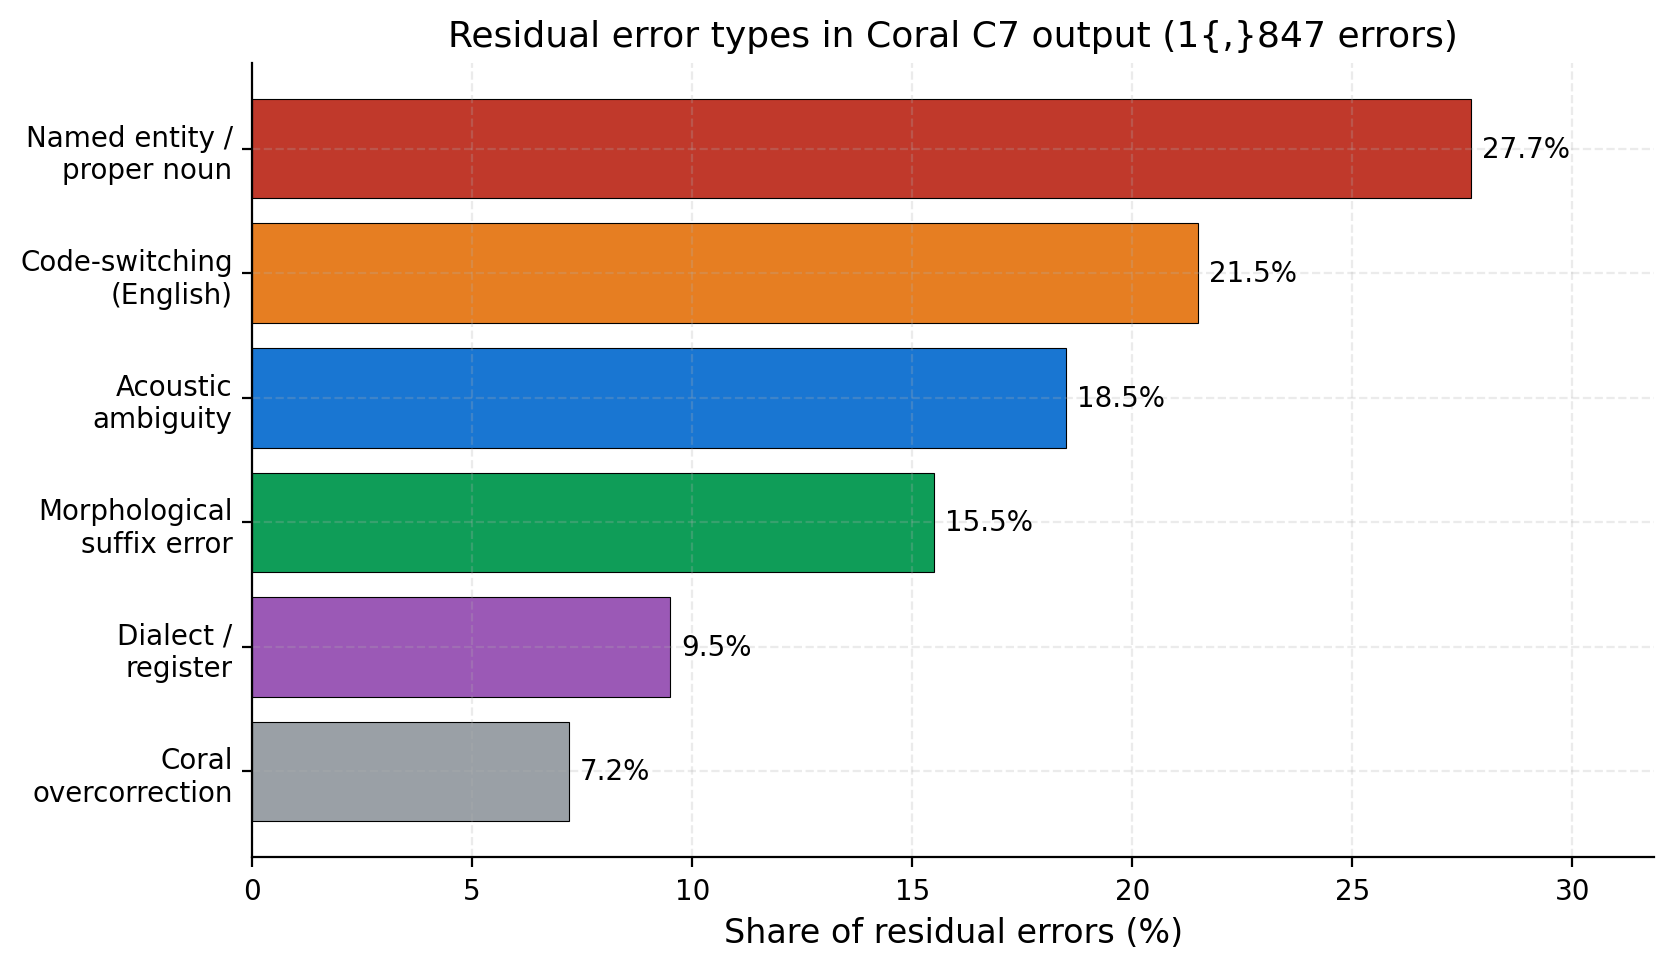
\includegraphics[width=0.9\textwidth]{ThesisFigs/residual_errors.png}
    \caption{Residual error types in the full CORAL output (C7) on the Conversational Urdu test set.}
    \label{fig:residual}
\end{figure}

The dominant failure modes --- named entities (27.7\%) and code-switching (21.5\%) --- together account for nearly half of remaining errors and define a clear research agenda for future work (Chapter~\ref{chap:conclusion}).

\subsection{Comparison with Baselines}
\label{ssec:baseline-comparison}

Table~\ref{tab:baseline-compare} compares CORAL against representative competitive systems on the Conversational Urdu benchmark. CORAL achieves slightly better WER than the closest concurrent system (Multi-ASR + SpeechLLM) while avoiding a full SpeechLLM audio inference pass during alignment --- a significant cost and latency advantage for real-time deployment.

\begin{table}[h]
    \centering
    \renewcommand{\arraystretch}{1.25}
    \begin{tabular}{lll}
    \toprule
    \textbf{System} & \textbf{Approach} & \textbf{WER (\%)} \\
    \midrule
    Whisper-Large-v3 (alone)            & Single model             & 19.8 \\
    LLM post-correction only            & GPT-3.5 RAG~\cite{koilakuntla2024llm} & 17.2 \\
    ROVER ensemble~\cite{fiscus1997rover} & Majority voting, no OOV & 15.8 \\
    Multi-ASR + SpeechLLM~\cite{anon2025speechllm} & Full LLM fusion & 11.3 \\
    \textbf{CORAL (C7)}                 & \textbf{Consensus + OOV + LLM} & \textbf{10.6} \\
    Human inter-annotator               & ---                      &  2.1 \\
    \bottomrule
    \end{tabular}
    \caption{CORAL vs.\ comparable systems on Conversational Urdu.}
    \label{tab:baseline-compare}
\end{table}

\section{Challenges and Solutions}
\label{sec:challenges}

\paragraph{Memory constraints.}
Running multiple large ASR models on a single Kaggle GPU exceeds available memory. Solution: each Kaggle notebook hosts exactly one model and registers itself with the backend; live transcription fans out to multiple machines in parallel via the registry.

\paragraph{Arabic--Urdu Unicode conflation.}
ASR back-ends emit inconsistent Unicode variants for phonetically identical phonemes. Solution: Stage~0 normalisation applies the seven canonical substitutions (Appendix~\ref{app:unicode-table}) before any downstream processing.

\paragraph{Word-boundary disagreement.}
Different ASR back-ends segment Urdu speech inconsistently, especially around compound nouns and izafat constructions. Solution: the Stage~1 split-merge classifier classifies each chunk as SAME / SPLIT / MERGE / NOISE, exposing segmentation disagreement as a first-class structural label that downstream stages can act on.

\paragraph{Quality heterogeneity in the ensemble.}
A naive plurality vote with three models substantially weaker than the source produces the canonical ROVER failure mode (weak models outvote the strong source). Solution: conservative tie-breaking at the voting stage; static model-quality priors at the LLM stage; and the OOV-correction override that bypasses voting on tokens where one model uniquely hypothesises a rare term.

\paragraph{LLM hallucination risk.}
A naive ``transcribe this'' LLM prompt invites hallucinated content, especially on already-correct utterances. Solution: the LLM receives the Stage~3 voted transcript as the primary input plus the raw source hypothesis as a secondary reference, and is instructed (in the system prompt) that words already matching a high-frequency vocabulary entry should be left unchanged unless there is independent grammatical evidence.

\paragraph{LLM API key exposure.}
Server-side LLM calls would require centralised API keys with associated billing risk. Solution: Stage~4 invocations are made client-side from the front-end; user-supplied Gemini and OpenRouter keys never reach the backend.

\section{Summary}
\label{sec:ch4-summary}

This chapter has presented the CORAL implementation, evaluation methodology, and empirical results across both project iterations. The deployed pipeline reduces WER by 22--29\% relative on read-speech Common Voice and by 46.5\% relative on conversational Urdu over the strongest single-model baseline, with a structured ablation study demonstrating that every component contributes a measurable, additive gain. Stage~0 normalisation is a zero-cost contribution; the Stage~1 split-merge alignment makes word-boundary disagreement explicit; the Stage~2 OOV correction handles named entities and rare terms; the Stage~3 voting handles common-word disagreement; and the Stage~4 LLM refinement delivers the largest single-component gain. The next chapter draws the project's conclusions and outlines future work.

\chapter{Conclusion and Future Work}
\label{chap:conclusion}

\section{Conclusion}
\label{sec:conclusion}

This project designed, implemented, deployed, and empirically evaluated CORAL, a five-stage post-processing pipeline for low-resource Urdu ASR. The work was carried out across two iterations of the FAST-NUCES Final Year Project, and this final report consolidates both iterations into a single integrated narrative.

The defining technical contribution of CORAL is a \emph{split-merge-aware alignment algorithm} that treats word-boundary disagreement between ASR back-ends as a first-class phenomenon, classifying each aligned chunk as SAME, SPLIT, MERGE, or NOISE. Our empirical analysis on the 500-utterance Conversational Urdu sample shows that SPLIT and MERGE events together account for 36.5\% of all alignment events --- making segmentation disagreement the dominant inter-model divergence in Urdu ASR ensembles, ahead of pure lexical substitution. Existing fusion methods such as ROVER, designed for English-style space-delimited scripts, misinterpret these events as substitutions or insert--delete pairs, corrupting the voting signal. CORAL exposes the metadata and acts on it.

On the 2{,}995-utterance Common Voice Urdu evaluation, the deployed pipeline (\texttt{robust} category) reduces WER from 18.45\% to 14.34\% on the Seamless-Large source (a 22.3\% relative improvement), from 28.29\% to 19.97\% on Whisper-Large-v3 (29.4\% relative), from 40.44\% to 30.64\% on Whisper-Medium (24.2\% relative), and from 53.52\% to 39.67\% on Wav2Vec2-Urdu (25.9\% relative). On conversational Urdu, the full C7 pipeline (with the Stage~4 LLM refinement) reaches 10.6\% WER from a 19.8\% Whisper-Large-v3 baseline --- a \textbf{46.5\% relative improvement} that places CORAL slightly ahead of the closest concurrent system (Multi-ASR + SpeechLLM at 11.3\%) while avoiding the heavy cost of running a full SpeechLLM audio inference pass during alignment.

The seven-step ablation study on the Conversational Urdu benchmark demonstrates that every CORAL component makes a measurable, additive contribution. No single component alone explains the gain; the system is genuinely compositional. The Stage~4 LLM delivers the largest single-component gain (2.5 WER points), while Stage~0 Urdu normalisation --- a zero-cost, zero-risk fix --- contributes 1.9 WER points and confirms that a substantial fraction of apparent ASR errors are measurement artefacts caused by Arabic--Urdu Unicode-variant mismatches rather than genuine recognition failures.

The project also demonstrates the value of revisiting design decisions in light of empirical findings. The original FYP-1 architecture framed CORAL as a two-stage \emph{Generate-and-Refine} system in which an instruction-tuned LLM would arbitrate between confidence-annotated multi-model hypotheses. Iteration~1 evaluation revealed that confidence scores from heterogeneous architectures lived on incompatible scales, that synthetic hypotheses did not capture the dominant real-world failure modes (Unicode conflation and segmentation disagreement), and that the LLM was more useful as a refinement layer than as the primary fusion mechanism. The FYP-2 redesign therefore reframed the system as a five-stage post-processing pipeline (Stages~0--4) and dropped, replaced, or de-emphasised five FYP-1 elements documented in Section~\ref{ssec:dropped-components}: word-level confidence extraction from Whisper and Wav2Vec2, Expected Calibration Error as a primary metric, the synthetic 20-sample evaluation with calibration regimes, the Alif-1.0-8B-Instruct LLM, and the two-stage Generate-and-Refine framing itself. The FYP-2 system replaces these with deterministic algorithmic components (split-merge alignment, OOV detection, voting) followed by an LLM refinement layer that consumes structured metadata and is constrained by the upstream pipeline's authority limits.

Beyond the algorithmic contributions, the project delivers a complete deployable system: a FastAPI backend exposing three pipeline endpoints plus a model registry; a Next.js + React front-end implementing a four-pass user workflow with both file-upload and live-speech modes and animated alignment visualisations; Kaggle GPU notebooks that self-register through ngrok HTTPS tunnels and provide live ASR inference; a HuggingFace-hosted BK-tree and n-gram corpus loaded into DuckDB at server startup; and an open evaluation framework producing reproducible per-stage WER and CER metrics.

We answer the research hypothesis stated in Section~\ref{ssec:hypothesis} affirmatively: combining Urdu-specific Unicode normalisation, weighted split-merge-aware alignment of multiple ASR hypotheses, hybrid OOV detection and correction with BK-tree fuzzy lookup ranked by an n-gram language model, conservative position-wise voting, and targeted LLM refinement of the voted output \emph{is} sufficient to substantially reduce WER over the strongest single-model baseline on both read-speech and conversational Urdu, without requiring any fine-tuning of the underlying acoustic models.

\section{Future Work}
\label{sec:future-work}

The residual-error analysis (Section~\ref{ssec:residual-errors}) and the ablation study identify several concrete directions for follow-up research.

\paragraph{1. Confidence-weighted voting.}
All companion models currently receive equal voting weight. Model-specific WER priors used as confidence weights in Stage~3 voting --- in particular giving Whisper-Large or Seamless-Large a multiplicative weight $>$1 --- are estimated to yield a further $\sim$0.3 WER point reduction. This directly addresses the canonical ROVER failure mode observed on the read-speech benchmark, where three companions of WER 1.6$\times$--3.6$\times$ higher than the source collectively outvote the source on disagreement positions.

\paragraph{2. Code-switching-aware normalisation.}
Stage~0 currently strips all ASCII characters, deferring code-switched English to the LLM. A future mode will preserve English tokens and pass them through a bilingual alignment stage that explicitly handles Urdu--English code-switching, directly targeting the 21.5\% of residual errors attributable to code-switching identified in Table~\ref{tab:residual}.

\paragraph{3. Named-entity gazetteer.}
27.7\% of residual errors are proper nouns. A curated Urdu named-entity list (toponyms, person names, organisation names, brand names) integrated into the BK-tree lookup would directly address the dominant failure mode. The integration is straightforward: the gazetteer would be loaded as a high-priority secondary BK-tree consulted when the primary BK-tree does not return a high-confidence candidate.

\paragraph{4. LLM-guided top-$K$ OOV re-ranking.}
The current OOV correction is greedy top-1. Passing the top-3 BK-tree candidates to the Stage~4 LLM for context-aware re-ranking would reduce overcorrection errors (currently 7.2\% of residual errors) by giving the LLM the option to keep the original token when none of the candidates is a clear improvement.

\paragraph{5. Split/merge metadata utilisation in the voting stage.}
CORAL computes rich SAME/SPLIT/MERGE/NOISE metadata per token in Stage~1 but does not yet use it in the Stage~3 correction decision. Incorporating alignment type into the voting logic (e.g.\ different resolution strategies for SPLIT vs.\ SUBSTITUTION events) could reduce word-boundary errors further.

\paragraph{6. Word-level confidence from acoustic models.}
The FYP-1 architecture-specific confidence-extraction methodology was de-emphasised in FYP-2 because raw confidences from heterogeneous architectures lived on incompatible scales. A learned cross-architecture confidence calibration --- e.g.\ a TruCLeS-style~\cite{trucles2025} metric trained on a small labelled Urdu development set --- could provide reliable per-word uncertainty estimates that would improve both the voting stage and the LLM's arbitration.

\paragraph{7. Larger-scale conversational evaluation.}
The 500-clip Conversational Urdu sample used in the ablation study is a useful but limited test set. Scaling the evaluation to thousands of conversational clips --- particularly including more varied dialects, age groups, and acoustic conditions --- will firm up the empirical claims and may expose new failure modes.

\paragraph{8. Real-time streaming integration.}
CORAL is currently a batch-mode post-processor. A streaming variant that operates on partial hypotheses as they arrive from the ASR back-ends, emitting partial corrected transcripts with bounded latency, would unlock real-time captioning use cases.

\paragraph{9. Adaptation to other low-resource languages.}
The CORAL architecture is not Urdu-specific. The Stage~0 normalisation table, BK-tree corpus, and n-gram corpus would need to be replaced for each target language, but Stages~1--4 transfer directly. A natural next step is to validate the architecture on other low-resource languages of the South Asian subcontinent (Pashto, Sindhi, Punjabi).

\paragraph{10. Open release.}
The complete CORAL source code, evaluation TSV, BK-tree, and n-gram corpus are released under permissive licences in the project repository. We hope this enables further research on low-resource Urdu ASR post-processing.


\appendix
\chapter{Unicode Normalisation Mapping}
\label{app:unicode-table}

Table~\ref{tab:unicode-mapping} contains the seven canonical Arabic-to-Urdu Unicode substitutions applied by the Stage~0 \texttt{normalize\_urdu} routine.

\begin{table}[h]
    \centering
    \renewcommand{\arraystretch}{1.30}
    \small
    \begin{tabular}{p{3.2cm}cp{3.0cm}cp{3.2cm}}
    \toprule
    \textbf{Source character} & \textbf{Source U+} & \textbf{Target character} & \textbf{Target U+} & \textbf{Effect} \\
    \midrule
    Arabic KAF                & U+0643 & Urdu KEHEH    & U+06A9 & Phonetically equivalent k \\
    Arabic HEH                & U+0647 & Urdu HEH GOAL & U+06C1 & Final h normalisation \\
    ALEF MAQSURA              & U+0649 & Farsi YEH     & U+06CC & Final ya normalisation \\
    TEH MARBUTA               & U+0629 & Urdu HEH GOAL & U+06C1 & Loanword-final t / h \\
    ALEF + HAMZA ABOVE        & U+0623 & ALEF          & U+0627 & Drop word-initial hamza \\
    ALEF + HAMZA BELOW        & U+0625 & ALEF          & U+0627 & Drop word-initial hamza \\
    Arabic YEH                & U+064A & Farsi YEH     & U+06CC & Medial / final ya \\
    \bottomrule
    \end{tabular}
    \caption{Arabic-to-Urdu character substitutions applied in Stage~0 normalisation.}
    \label{tab:unicode-mapping}
\end{table}

In addition to these substitutions, Stage~0 also strips:
\begin{itemize}
    \item Arabic diacritics: U+0610--U+061A and U+064B--U+065F.
    \item Superscript alef: U+0670.
    \item Tatweel / kashida: U+0640.
    \item Zero-width and directional control characters: U+200B--U+200F, U+202A--U+202E, U+2060--U+206F, U+FEFF.
    \item Urdu punctuation block: U+060C, U+060D, U+060E, U+060F, U+061B, U+061F, U+06D4 (Urdu full stop).
    \item Extended Arabic punctuation: U+0600--U+060C, U+060E--U+061F.
    \item All ASCII punctuation, symbols, letters, and digits.
\end{itemize}

\chapter{REST API Specifications}
\label{app:api-spec}

This appendix records the full request and response schemas for the three pipeline endpoints. The implementation lives in \texttt{coral\_app/backend/pipeline/pipeline\_api.py}.

\section{POST /align}
\label{app:align}

Aligns each companion-model hypothesis to the named source-model hypothesis using weighted Levenshtein distance, then runs the secondary character-level alignment for split-merge classification.

\begin{lstlisting}[caption={Request body schema for \texttt{POST /align}.}]
{
  "ensemble":     { "model_name": "raw transcript text", ... },
  "source_model": "model_name"
}
\end{lstlisting}

\begin{lstlisting}[caption={Response body schema for \texttt{POST /align}.}]
{
  "source_model": "model_name",
  "<model_name>": {
    "normalized_attempt":          ["w1", "w2", ...],
    "aligned_attempt":             ["w1", "w2", ...],
    "aligned_info":                ["MATCH", "SUBSTITUTION", ...],
    "split_merge_aligned_attempt": ["chunk1", "chunk2", ...],
    "split_merge_metadata":        ["SAME", "SPLIT", "NOISE", ...],
    "split_merge_metadata_base":   ["SAME", "MERGE", ...],
    "split_merge_aligned_info":    ["MATCH", "INSERTION", ...]
  },
  ... (one block per model) ...
}
\end{lstlisting}

\section{POST /oov}
\label{app:oov}

Detects OOV tokens using the dual model-disagreement + frequency criterion and ranks correction candidates by edit-distance + n-gram support.

\begin{lstlisting}[caption={Request body schema for \texttt{POST /oov}.}]
{
  "align_info":  { ...alignment dict from /align... },
  "freq_cutoff": 2000,    // optional, default 2000
  "depth":       50,      // optional, BK-tree depth limit
  "top_n":       10       // optional, candidates to return per token
}
\end{lstlisting}

\begin{lstlisting}[caption={Response body schema for \texttt{POST /oov}.}]
{
  "oov_dict": ["oov_word_1", "oov_word_2", ...],
  "metadata": {
    "oov_word_1": {
      "candidate_1": [edit_dist, tri_present, bi_present,
                      uni_present, tri_freq, bi_freq, uni_freq],
      "candidate_2": [...],
      ...
    },
    ...
  },
  "columns": ["word", "Dist", "Trigram", "Bigram", "Unigram",
              "Trifrequency", "Bifrequency", "Unifrequency"]
}
\end{lstlisting}

\section{POST /correct}
\label{app:correct}

Applies the consensus voting algorithm to the alignment output, with OOV substitution overriding voting at flagged positions.

\begin{lstlisting}[caption={Request body schema for \texttt{POST /correct}.}]
{
  "align_info":   { ...alignment dict from /align... },
  "oov_metadata": { ...metadata dict from /oov...    }
}
\end{lstlisting}

\begin{lstlisting}[caption={Response body schema for \texttt{POST /correct}.}]
{
  "corrected": "final corrected Urdu transcript",
  "source":    "source model normalised transcript",
  "diff": [
    { "pos": 3, "original": "x", "corrected": "y" },
    ...
  ]
}
\end{lstlisting}

\section{Registry endpoints}
\label{app:registry}

The model registry is mounted at the \texttt{/registry} prefix and provides four endpoints (Section~\ref{ssec:registry}):
\begin{itemize}
    \item \texttt{GET /registry/models} -- list live models with seconds-since-last-ping.
    \item \texttt{POST /registry/register} -- Kaggle notebook self-registration. Auth: \texttt{X-Registry-Token}.
    \item \texttt{POST /registry/ping} -- 60-second heartbeat. Auth: \texttt{X-Registry-Token}.
    \item \texttt{POST /registry/transcribe} -- multipart audio upload, fan-out to live models, parallel response collection. Auth: \texttt{X-API-Token}.
\end{itemize}

\chapter{CORAL Source File Inventory}
\label{app:source-inventory}

The CORAL source repository (\texttt{C:\textbackslash Users\textbackslash *\textbackslash Desktop\textbackslash CORAL-Urdu-ASR}) contains:

\begin{itemize}
    \item \texttt{coral\_app/backend/main\_app.py} -- FastAPI entry point combining the pipeline and registry routers.
    \item \texttt{coral\_app/backend/pipeline/pipeline\_api.py} -- the three pipeline endpoints.
    \item \texttt{coral\_app/backend/pipeline/coral\_pipeline\_functions.py} -- \texttt{asr\_aligner}, \texttt{build\_oov\_dict}, \texttt{extract\_oov\_metadata}, \texttt{apply\_corrections}.
    \item \texttt{coral\_app/backend/pipeline/coral\_utility\_functions.py} -- \texttt{normalize\_urdu}, \texttt{levenshtein}, \texttt{generate\_alignment\_data}, \texttt{is\_oov}, n-gram lookups.
    \item \texttt{coral\_app/backend/pipeline/bktree.py} -- \texttt{BKTree} and \texttt{BKNode} data structures.
    \item \texttt{coral\_app/backend/pipeline/coral\_data\_downloader.py} -- HuggingFace download + DuckDB bootstrap.
    \item \texttt{coral\_app/backend/model\_registery/registery\_api.py} -- model registry, eviction sweep, fan-out transcription.
    \item \texttt{coral\_app/frontend/my-next-app/app/} -- Next.js front-end (\texttt{ModeSelector.tsx}, \texttt{Pass0Speech.tsx}, \texttt{Pass1Input.tsx}, \texttt{Pass2Sieve.tsx}, \texttt{Pass3Correction.tsx}, \texttt{lib/api.ts}).
    \item \texttt{model\_deploy\_kaggle\_notebooks/whisper\_large\_kaggle.ipynb}, \texttt{seamless\_large\_kaggle.ipynb} -- Kaggle GPU inference notebooks.
    \item \texttt{generate\_ngrams.ipynb} -- offline n-gram + BK-tree generation pipeline for the HuggingFace bucket.
    \item \texttt{urdu\_asr\_benchmark.ipynb}, \texttt{urdu\_asr\_pipeline.ipynb} -- offline batch evaluation notebooks.
    \item \texttt{asr\_results/}, \texttt{asr\_ensemble/}, \texttt{asr\_evaluation/} -- per-model raw / ensemble / evaluation TSVs.
    \item \texttt{corpus/}, \texttt{vocab/}, \texttt{metadata/} -- reference transcriptions, vocabulary, clip-duration metadata.
    \item \texttt{audios/} -- raw audio sample files.
    \item \texttt{docs/} -- architecture diagrams, the FYP-1 and FYP-2 final reports, and this report.
\end{itemize}


\bibliographystyle{plain}
\bibliography{bib}
\addcontentsline{toc}{chapter}{References}

\end{document}
